\documentclass[twoside]{book}

% Packages required by doxygen
\usepackage{fixltx2e}
\usepackage{calc}
\usepackage{doxygen}
\usepackage[export]{adjustbox} % also loads graphicx
\usepackage{graphicx}
\usepackage[utf8]{inputenc}
\usepackage{makeidx}
\usepackage{multicol}
\usepackage{multirow}
\PassOptionsToPackage{warn}{textcomp}
\usepackage{textcomp}
\usepackage[nointegrals]{wasysym}
\usepackage[table]{xcolor}

% Font selection
\usepackage[T1]{fontenc}
\usepackage[scaled=.90]{helvet}
\usepackage{courier}
\usepackage{amssymb}
\usepackage{sectsty}
\renewcommand{\familydefault}{\sfdefault}
\allsectionsfont{%
  \fontseries{bc}\selectfont%
  \color{darkgray}%
}
\renewcommand{\DoxyLabelFont}{%
  \fontseries{bc}\selectfont%
  \color{darkgray}%
}
\newcommand{\+}{\discretionary{\mbox{\scriptsize$\hookleftarrow$}}{}{}}

% Page & text layout
\usepackage{geometry}
\geometry{%
  a4paper,%
  top=2.5cm,%
  bottom=2.5cm,%
  left=2.5cm,%
  right=2.5cm%
}
\tolerance=750
\hfuzz=15pt
\hbadness=750
\setlength{\emergencystretch}{15pt}
\setlength{\parindent}{0cm}
\setlength{\parskip}{3ex plus 2ex minus 2ex}
\makeatletter
\renewcommand{\paragraph}{%
  \@startsection{paragraph}{4}{0ex}{-1.0ex}{1.0ex}{%
    \normalfont\normalsize\bfseries\SS@parafont%
  }%
}
\renewcommand{\subparagraph}{%
  \@startsection{subparagraph}{5}{0ex}{-1.0ex}{1.0ex}{%
    \normalfont\normalsize\bfseries\SS@subparafont%
  }%
}
\makeatother

% Headers & footers
\usepackage{fancyhdr}
\pagestyle{fancyplain}
\fancyhead[LE]{\fancyplain{}{\bfseries\thepage}}
\fancyhead[CE]{\fancyplain{}{}}
\fancyhead[RE]{\fancyplain{}{\bfseries\leftmark}}
\fancyhead[LO]{\fancyplain{}{\bfseries\rightmark}}
\fancyhead[CO]{\fancyplain{}{}}
\fancyhead[RO]{\fancyplain{}{\bfseries\thepage}}
\fancyfoot[LE]{\fancyplain{}{}}
\fancyfoot[CE]{\fancyplain{}{}}
\fancyfoot[RE]{\fancyplain{}{\bfseries\scriptsize Generated by Doxygen }}
\fancyfoot[LO]{\fancyplain{}{\bfseries\scriptsize Generated by Doxygen }}
\fancyfoot[CO]{\fancyplain{}{}}
\fancyfoot[RO]{\fancyplain{}{}}
\renewcommand{\footrulewidth}{0.4pt}
\renewcommand{\chaptermark}[1]{%
  \markboth{#1}{}%
}
\renewcommand{\sectionmark}[1]{%
  \markright{\thesection\ #1}%
}

% Indices & bibliography
\usepackage{natbib}
\usepackage[titles]{tocloft}
\setcounter{tocdepth}{3}
\setcounter{secnumdepth}{5}
\makeindex

% Hyperlinks (required, but should be loaded last)
\usepackage{ifpdf}
\ifpdf
  \usepackage[pdftex,pagebackref=true]{hyperref}
\else
  \usepackage[ps2pdf,pagebackref=true]{hyperref}
\fi
\hypersetup{%
  colorlinks=true,%
  linkcolor=blue,%
  citecolor=blue,%
  unicode%
}

% Custom commands
\newcommand{\clearemptydoublepage}{%
  \newpage{\pagestyle{empty}\cleardoublepage}%
}

\usepackage{caption}
\captionsetup{labelsep=space,justification=centering,font={bf},singlelinecheck=off,skip=4pt,position=top}

%===== C O N T E N T S =====

\begin{document}

% Titlepage & ToC
\hypersetup{pageanchor=false,
             bookmarksnumbered=true,
             pdfencoding=unicode
            }
\pagenumbering{alph}
\begin{titlepage}
\vspace*{7cm}
\begin{center}%
{\Large Project Low\+Blow Thermal Controller Setup Tool }\\
\vspace*{1cm}
{\large Generated by Doxygen 1.8.13}\\
\end{center}
\end{titlepage}
\clearemptydoublepage
\pagenumbering{roman}
\tableofcontents
\clearemptydoublepage
\pagenumbering{arabic}
\hypersetup{pageanchor=true}

%--- Begin generated contents ---
\chapter{Namespace Index}
\section{Namespace List}
Here is a list of all documented namespaces with brief descriptions\+:\begin{DoxyCompactList}
\item\contentsline{section}{\hyperlink{namespace_fossa}{Fossa} \\*Namespace for all reusable stuff, created by \hyperlink{namespace_fossa}{Fossa} }{\pageref{namespace_fossa}}{}
\item\contentsline{section}{\hyperlink{namespace_fossa_1_1_q_simple_graph}{Fossa\+::\+Q\+Simple\+Graph} \\*Simple graph control }{\pageref{namespace_fossa_1_1_q_simple_graph}}{}
\item\contentsline{section}{\hyperlink{namespace_fossa_1_1_q_simple_graph_1_1_interfaces}{Fossa\+::\+Q\+Simple\+Graph\+::\+Interfaces} \\*Simple graph control interfaces }{\pageref{namespace_fossa_1_1_q_simple_graph_1_1_interfaces}}{}
\item\contentsline{section}{\hyperlink{namespace_ui}{Ui} }{\pageref{namespace_ui}}{}
\end{DoxyCompactList}

\chapter{Hierarchical Index}
\section{Class Hierarchy}
This inheritance list is sorted roughly, but not completely, alphabetically\+:\begin{DoxyCompactList}
\item Q\+Dialog\begin{DoxyCompactList}
\item \contentsline{section}{New\+A\+D\+C2\+Temp\+Dialog}{\pageref{class_new_a_d_c2_temp_dialog}}{}
\end{DoxyCompactList}
\item Q\+Main\+Window\begin{DoxyCompactList}
\item \contentsline{section}{Main\+Window}{\pageref{class_main_window}}{}
\end{DoxyCompactList}
\item Q\+Object\begin{DoxyCompactList}
\item \contentsline{section}{Interfaces\+:\+:I\+Adc\+Temperature\+Convertor}{\pageref{class_interfaces_1_1_i_adc_temperature_convertor}}{}
\begin{DoxyCompactList}
\item \contentsline{section}{Adc\+Temperature\+Convertor}{\pageref{class_adc_temperature_convertor}}{}
\end{DoxyCompactList}
\item \contentsline{section}{Interfaces\+:\+:I\+Settings\+Generator}{\pageref{class_interfaces_1_1_i_settings_generator}}{}
\begin{DoxyCompactList}
\item \contentsline{section}{Settings\+Generator}{\pageref{class_settings_generator}}{}
\end{DoxyCompactList}
\item \contentsline{section}{Interfaces\+:\+:I\+Settings\+Step}{\pageref{class_interfaces_1_1_i_settings_step}}{}
\begin{DoxyCompactList}
\item \contentsline{section}{Settings\+Step}{\pageref{class_settings_step}}{}
\end{DoxyCompactList}
\end{DoxyCompactList}
\item Q\+Widget\begin{DoxyCompactList}
\item \contentsline{section}{Fossa\+:\+:Q\+Simple\+Graph\+:\+:Interfaces\+:\+:I\+Q\+Simple\+Graph}{\pageref{class_fossa_1_1_q_simple_graph_1_1_interfaces_1_1_i_q_simple_graph}}{}
\begin{DoxyCompactList}
\item \contentsline{section}{Fossa\+:\+:Q\+Simple\+Graph\+:\+:Q\+Simple\+Graph}{\pageref{class_fossa_1_1_q_simple_graph_1_1_q_simple_graph}}{}
\end{DoxyCompactList}
\end{DoxyCompactList}
\end{DoxyCompactList}

\chapter{Class Index}
\section{Class List}
Here are the classes, structs, unions and interfaces with brief descriptions\+:\begin{DoxyCompactList}
\item\contentsline{section}{\hyperlink{class_adc_temperature_convertor}{Adc\+Temperature\+Convertor} \\*Implementation of \hyperlink{class_interfaces_1_1_i_adc_temperature_convertor}{Interfaces\+::\+I\+Adc\+Temperature\+Convertor} }{\pageref{class_adc_temperature_convertor}}{}
\item\contentsline{section}{\hyperlink{class_interfaces_1_1_i_adc_temperature_convertor}{Interfaces\+::\+I\+Adc\+Temperature\+Convertor} \\*Class, used to convert A\+DC values to Temperature and vice versa }{\pageref{class_interfaces_1_1_i_adc_temperature_convertor}}{}
\item\contentsline{section}{\hyperlink{class_fossa_1_1_q_simple_graph_1_1_interfaces_1_1_i_q_simple_graph}{Fossa\+::\+Q\+Simple\+Graph\+::\+Interfaces\+::\+I\+Q\+Simple\+Graph} \\*Main interface of \hyperlink{class_fossa_1_1_q_simple_graph_1_1_q_simple_graph}{Q\+Simple\+Graph} }{\pageref{class_fossa_1_1_q_simple_graph_1_1_interfaces_1_1_i_q_simple_graph}}{}
\item\contentsline{section}{\hyperlink{class_interfaces_1_1_i_settings_generator}{Interfaces\+::\+I\+Settings\+Generator} \\*Class, containing all settings steps. It being used to generate settings table, which will be converted to E\+E\+P\+R\+OM data }{\pageref{class_interfaces_1_1_i_settings_generator}}{}
\item\contentsline{section}{\hyperlink{class_interfaces_1_1_i_settings_saver_loader}{Interfaces\+::\+I\+Settings\+Saver\+Loader} \\*Class to save and load controller settings into X\+ML }{\pageref{class_interfaces_1_1_i_settings_saver_loader}}{}
\item\contentsline{section}{\hyperlink{class_interfaces_1_1_i_settings_step}{Interfaces\+::\+I\+Settings\+Step} \\*Class with one settings step (i.\+e. with temperature and R\+PM percent increments) }{\pageref{class_interfaces_1_1_i_settings_step}}{}
\item\contentsline{section}{\hyperlink{class_main_window}{Main\+Window} }{\pageref{class_main_window}}{}
\item\contentsline{section}{\hyperlink{class_new_a_d_c2_temp_dialog}{New\+A\+D\+C2\+Temp\+Dialog} }{\pageref{class_new_a_d_c2_temp_dialog}}{}
\item\contentsline{section}{\hyperlink{class_fossa_1_1_q_simple_graph_1_1_q_simple_graph}{Fossa\+::\+Q\+Simple\+Graph\+::\+Q\+Simple\+Graph} \\*\hyperlink{class_fossa_1_1_q_simple_graph_1_1_q_simple_graph}{Q\+Simple\+Graph} widget implementation }{\pageref{class_fossa_1_1_q_simple_graph_1_1_q_simple_graph}}{}
\item\contentsline{section}{\hyperlink{class_settings_generator}{Settings\+Generator} \\*Class, being used to generate settings (see Interfaces/\+I\+Settings\+Generator for information) }{\pageref{class_settings_generator}}{}
\item\contentsline{section}{\hyperlink{class_settings_saver_loader}{Settings\+Saver\+Loader} \\*Class to save and load settings to X\+ML }{\pageref{class_settings_saver_loader}}{}
\item\contentsline{section}{\hyperlink{class_settings_step}{Settings\+Step} \\*Class with one settings step (see Interfaces/\+I\+Settings\+Step for information) }{\pageref{class_settings_step}}{}
\item\contentsline{section}{\hyperlink{class_fossa_1_1_helpers_1_1_xml_helper}{Fossa\+::\+Helpers\+::\+Xml\+Helper} \\*Helper class to work with X\+ML (parse it, to be precise) }{\pageref{class_fossa_1_1_helpers_1_1_xml_helper}}{}
\end{DoxyCompactList}

\chapter{Namespace Documentation}
\hypertarget{namespace_fossa}{}\section{Fossa Namespace Reference}
\label{namespace_fossa}\index{Fossa@{Fossa}}


Namespace for all reusable stuff, created by \hyperlink{namespace_fossa}{Fossa}.  


\subsection*{Namespaces}
\begin{DoxyCompactItemize}
\item 
 \hyperlink{namespace_fossa_1_1_q_simple_graph}{Q\+Simple\+Graph}
\begin{DoxyCompactList}\small\item\em Simple graph control. \end{DoxyCompactList}\end{DoxyCompactItemize}


\subsection{Detailed Description}
Namespace for all reusable stuff, created by \hyperlink{namespace_fossa}{Fossa}. 

Define it to draw point-\/to-\/point graph instead of ladder one. 
\hypertarget{namespace_fossa_1_1_q_simple_graph}{}\section{Fossa\+:\+:Q\+Simple\+Graph Namespace Reference}
\label{namespace_fossa_1_1_q_simple_graph}\index{Fossa\+::\+Q\+Simple\+Graph@{Fossa\+::\+Q\+Simple\+Graph}}


Simple graph control.  


\subsection*{Namespaces}
\begin{DoxyCompactItemize}
\item 
 \hyperlink{namespace_fossa_1_1_q_simple_graph_1_1_interfaces}{Interfaces}
\begin{DoxyCompactList}\small\item\em Simple graph control interfaces. \end{DoxyCompactList}\end{DoxyCompactItemize}
\subsection*{Classes}
\begin{DoxyCompactItemize}
\item 
class \hyperlink{class_fossa_1_1_q_simple_graph_1_1_q_simple_graph}{Q\+Simple\+Graph}
\begin{DoxyCompactList}\small\item\em \hyperlink{class_fossa_1_1_q_simple_graph_1_1_q_simple_graph}{Q\+Simple\+Graph} widget implementation. \end{DoxyCompactList}\end{DoxyCompactItemize}
\subsection*{Enumerations}
\begin{DoxyCompactItemize}
\item 
\mbox{\Hypertarget{namespace_fossa_1_1_q_simple_graph_a0c50b3eb82acac4a64e9b291c8f1b7cc}\label{namespace_fossa_1_1_q_simple_graph_a0c50b3eb82acac4a64e9b291c8f1b7cc}} 
enum \hyperlink{namespace_fossa_1_1_q_simple_graph_a0c50b3eb82acac4a64e9b291c8f1b7cc}{Tooltip\+Direction} \{ {\bfseries Up\+Left}, 
{\bfseries Up\+Right}, 
{\bfseries Down\+Left}, 
{\bfseries Down\+Right}
 \}\begin{DoxyCompactList}\small\item\em Possible tooltip directions relative to target point. \end{DoxyCompactList}
\end{DoxyCompactItemize}


\subsection{Detailed Description}
Simple graph control. 
\hypertarget{namespace_fossa_1_1_q_simple_graph_1_1_interfaces}{}\section{Fossa\+:\+:Q\+Simple\+Graph\+:\+:Interfaces Namespace Reference}
\label{namespace_fossa_1_1_q_simple_graph_1_1_interfaces}\index{Fossa\+::\+Q\+Simple\+Graph\+::\+Interfaces@{Fossa\+::\+Q\+Simple\+Graph\+::\+Interfaces}}


Simple graph control interfaces.  


\subsection*{Classes}
\begin{DoxyCompactItemize}
\item 
class \hyperlink{class_fossa_1_1_q_simple_graph_1_1_interfaces_1_1_i_q_simple_graph}{I\+Q\+Simple\+Graph}
\begin{DoxyCompactList}\small\item\em Main interface of \hyperlink{class_fossa_1_1_q_simple_graph_1_1_q_simple_graph}{Q\+Simple\+Graph}. \end{DoxyCompactList}\end{DoxyCompactItemize}


\subsection{Detailed Description}
Simple graph control interfaces. 
\hypertarget{namespace_ui}{}\section{Ui Namespace Reference}
\label{namespace_ui}\index{Ui@{Ui}}
\subsection*{Enumerations}
\begin{DoxyCompactItemize}
\item 
enum \hyperlink{namespace_ui_ab417c7821a7da9a52d574ee5e2ecf6f0}{S\+T\+E\+P\+S\+\_\+\+T\+A\+B\+L\+E\+\_\+\+R\+O\+WS} \{ \newline
\hyperlink{namespace_ui_ab417c7821a7da9a52d574ee5e2ecf6f0a3ce827b16c92c4223079c8f5e81ae264}{A\+D\+C\+\_\+\+L\+E\+V\+EL} = 0, 
\hyperlink{namespace_ui_ab417c7821a7da9a52d574ee5e2ecf6f0a95e4957d31702a84bca284e48318efd1}{T\+E\+M\+P\+E\+R\+A\+T\+U\+RE} = 1, 
\hyperlink{namespace_ui_ab417c7821a7da9a52d574ee5e2ecf6f0ac6f609b55b214ac58aa0b2f702a3244f}{R\+P\+M\+\_\+\+L\+E\+V\+EL} = 2, 
\hyperlink{namespace_ui_ab417c7821a7da9a52d574ee5e2ecf6f0a25e4220b0ee49ef66eb7c76fae978aa6}{R\+P\+M\+\_\+\+P\+E\+R\+C\+E\+NT} = 3, 
\newline
\hyperlink{namespace_ui_ab417c7821a7da9a52d574ee5e2ecf6f0aa34e92bd0beb0f4723495c66ce9c676e}{A\+D\+C\+\_\+\+D\+E\+L\+TA} = 4, 
\hyperlink{namespace_ui_ab417c7821a7da9a52d574ee5e2ecf6f0a7d1306709fbe1b5d00d6792f3a1e9ae1}{T\+E\+M\+P\+E\+R\+A\+T\+U\+R\+E\+\_\+\+D\+E\+L\+TA} = 5, 
\hyperlink{namespace_ui_ab417c7821a7da9a52d574ee5e2ecf6f0aa810bf7a4e77e6c834b2bf7f956429ac}{R\+P\+M\+\_\+\+D\+E\+L\+TA} = 6, 
\hyperlink{namespace_ui_ab417c7821a7da9a52d574ee5e2ecf6f0af4e0e9ab0dbab7f2cad423ad7f315d1b}{R\+P\+M\+\_\+\+D\+E\+L\+T\+A\+\_\+\+P\+E\+R\+C\+E\+NT} = 7
 \}\begin{DoxyCompactList}\small\item\em Columns of Steps Table (ui-\/$>$mw\+\_\+\+Steps\+Table) \end{DoxyCompactList}
\end{DoxyCompactItemize}


\subsection{Detailed Description}
Main window class

New A\+DC to Temperature settings dialog 

\subsection{Enumeration Type Documentation}
\mbox{\Hypertarget{namespace_ui_ab417c7821a7da9a52d574ee5e2ecf6f0}\label{namespace_ui_ab417c7821a7da9a52d574ee5e2ecf6f0}} 
\index{Ui@{Ui}!S\+T\+E\+P\+S\+\_\+\+T\+A\+B\+L\+E\+\_\+\+R\+O\+WS@{S\+T\+E\+P\+S\+\_\+\+T\+A\+B\+L\+E\+\_\+\+R\+O\+WS}}
\index{S\+T\+E\+P\+S\+\_\+\+T\+A\+B\+L\+E\+\_\+\+R\+O\+WS@{S\+T\+E\+P\+S\+\_\+\+T\+A\+B\+L\+E\+\_\+\+R\+O\+WS}!Ui@{Ui}}
\subsubsection{\texorpdfstring{S\+T\+E\+P\+S\+\_\+\+T\+A\+B\+L\+E\+\_\+\+R\+O\+WS}{STEPS\_TABLE\_ROWS}}
{\footnotesize\ttfamily enum \hyperlink{namespace_ui_ab417c7821a7da9a52d574ee5e2ecf6f0}{Ui\+::\+S\+T\+E\+P\+S\+\_\+\+T\+A\+B\+L\+E\+\_\+\+R\+O\+WS}}



Columns of Steps Table (ui-\/$>$mw\+\_\+\+Steps\+Table) 

\begin{DoxyEnumFields}{Enumerator}
\raisebox{\heightof{T}}[0pt][0pt]{\index{A\+D\+C\+\_\+\+L\+E\+V\+EL@{A\+D\+C\+\_\+\+L\+E\+V\+EL}!Ui@{Ui}}\index{Ui@{Ui}!A\+D\+C\+\_\+\+L\+E\+V\+EL@{A\+D\+C\+\_\+\+L\+E\+V\+EL}}}\mbox{\Hypertarget{namespace_ui_ab417c7821a7da9a52d574ee5e2ecf6f0a3ce827b16c92c4223079c8f5e81ae264}\label{namespace_ui_ab417c7821a7da9a52d574ee5e2ecf6f0a3ce827b16c92c4223079c8f5e81ae264}} 
A\+D\+C\+\_\+\+L\+E\+V\+EL&Row with A\+DC level \\
\hline

\raisebox{\heightof{T}}[0pt][0pt]{\index{T\+E\+M\+P\+E\+R\+A\+T\+U\+RE@{T\+E\+M\+P\+E\+R\+A\+T\+U\+RE}!Ui@{Ui}}\index{Ui@{Ui}!T\+E\+M\+P\+E\+R\+A\+T\+U\+RE@{T\+E\+M\+P\+E\+R\+A\+T\+U\+RE}}}\mbox{\Hypertarget{namespace_ui_ab417c7821a7da9a52d574ee5e2ecf6f0a95e4957d31702a84bca284e48318efd1}\label{namespace_ui_ab417c7821a7da9a52d574ee5e2ecf6f0a95e4957d31702a84bca284e48318efd1}} 
T\+E\+M\+P\+E\+R\+A\+T\+U\+RE&Row with temperature \\
\hline

\raisebox{\heightof{T}}[0pt][0pt]{\index{R\+P\+M\+\_\+\+L\+E\+V\+EL@{R\+P\+M\+\_\+\+L\+E\+V\+EL}!Ui@{Ui}}\index{Ui@{Ui}!R\+P\+M\+\_\+\+L\+E\+V\+EL@{R\+P\+M\+\_\+\+L\+E\+V\+EL}}}\mbox{\Hypertarget{namespace_ui_ab417c7821a7da9a52d574ee5e2ecf6f0ac6f609b55b214ac58aa0b2f702a3244f}\label{namespace_ui_ab417c7821a7da9a52d574ee5e2ecf6f0ac6f609b55b214ac58aa0b2f702a3244f}} 
R\+P\+M\+\_\+\+L\+E\+V\+EL&Row with R\+PM level \\
\hline

\raisebox{\heightof{T}}[0pt][0pt]{\index{R\+P\+M\+\_\+\+P\+E\+R\+C\+E\+NT@{R\+P\+M\+\_\+\+P\+E\+R\+C\+E\+NT}!Ui@{Ui}}\index{Ui@{Ui}!R\+P\+M\+\_\+\+P\+E\+R\+C\+E\+NT@{R\+P\+M\+\_\+\+P\+E\+R\+C\+E\+NT}}}\mbox{\Hypertarget{namespace_ui_ab417c7821a7da9a52d574ee5e2ecf6f0a25e4220b0ee49ef66eb7c76fae978aa6}\label{namespace_ui_ab417c7821a7da9a52d574ee5e2ecf6f0a25e4220b0ee49ef66eb7c76fae978aa6}} 
R\+P\+M\+\_\+\+P\+E\+R\+C\+E\+NT&Row with R\+PM percent \\
\hline

\raisebox{\heightof{T}}[0pt][0pt]{\index{A\+D\+C\+\_\+\+D\+E\+L\+TA@{A\+D\+C\+\_\+\+D\+E\+L\+TA}!Ui@{Ui}}\index{Ui@{Ui}!A\+D\+C\+\_\+\+D\+E\+L\+TA@{A\+D\+C\+\_\+\+D\+E\+L\+TA}}}\mbox{\Hypertarget{namespace_ui_ab417c7821a7da9a52d574ee5e2ecf6f0aa34e92bd0beb0f4723495c66ce9c676e}\label{namespace_ui_ab417c7821a7da9a52d574ee5e2ecf6f0aa34e92bd0beb0f4723495c66ce9c676e}} 
A\+D\+C\+\_\+\+D\+E\+L\+TA&Row with A\+DC level increase \\
\hline

\raisebox{\heightof{T}}[0pt][0pt]{\index{T\+E\+M\+P\+E\+R\+A\+T\+U\+R\+E\+\_\+\+D\+E\+L\+TA@{T\+E\+M\+P\+E\+R\+A\+T\+U\+R\+E\+\_\+\+D\+E\+L\+TA}!Ui@{Ui}}\index{Ui@{Ui}!T\+E\+M\+P\+E\+R\+A\+T\+U\+R\+E\+\_\+\+D\+E\+L\+TA@{T\+E\+M\+P\+E\+R\+A\+T\+U\+R\+E\+\_\+\+D\+E\+L\+TA}}}\mbox{\Hypertarget{namespace_ui_ab417c7821a7da9a52d574ee5e2ecf6f0a7d1306709fbe1b5d00d6792f3a1e9ae1}\label{namespace_ui_ab417c7821a7da9a52d574ee5e2ecf6f0a7d1306709fbe1b5d00d6792f3a1e9ae1}} 
T\+E\+M\+P\+E\+R\+A\+T\+U\+R\+E\+\_\+\+D\+E\+L\+TA&Row with temperature increase \\
\hline

\raisebox{\heightof{T}}[0pt][0pt]{\index{R\+P\+M\+\_\+\+D\+E\+L\+TA@{R\+P\+M\+\_\+\+D\+E\+L\+TA}!Ui@{Ui}}\index{Ui@{Ui}!R\+P\+M\+\_\+\+D\+E\+L\+TA@{R\+P\+M\+\_\+\+D\+E\+L\+TA}}}\mbox{\Hypertarget{namespace_ui_ab417c7821a7da9a52d574ee5e2ecf6f0aa810bf7a4e77e6c834b2bf7f956429ac}\label{namespace_ui_ab417c7821a7da9a52d574ee5e2ecf6f0aa810bf7a4e77e6c834b2bf7f956429ac}} 
R\+P\+M\+\_\+\+D\+E\+L\+TA&Row with R\+PM level increase \\
\hline

\raisebox{\heightof{T}}[0pt][0pt]{\index{R\+P\+M\+\_\+\+D\+E\+L\+T\+A\+\_\+\+P\+E\+R\+C\+E\+NT@{R\+P\+M\+\_\+\+D\+E\+L\+T\+A\+\_\+\+P\+E\+R\+C\+E\+NT}!Ui@{Ui}}\index{Ui@{Ui}!R\+P\+M\+\_\+\+D\+E\+L\+T\+A\+\_\+\+P\+E\+R\+C\+E\+NT@{R\+P\+M\+\_\+\+D\+E\+L\+T\+A\+\_\+\+P\+E\+R\+C\+E\+NT}}}\mbox{\Hypertarget{namespace_ui_ab417c7821a7da9a52d574ee5e2ecf6f0af4e0e9ab0dbab7f2cad423ad7f315d1b}\label{namespace_ui_ab417c7821a7da9a52d574ee5e2ecf6f0af4e0e9ab0dbab7f2cad423ad7f315d1b}} 
R\+P\+M\+\_\+\+D\+E\+L\+T\+A\+\_\+\+P\+E\+R\+C\+E\+NT&Row with R\+PM level increase in percents \\
\hline

\end{DoxyEnumFields}


Definition at line 45 of file mainwindow.\+hpp.


\chapter{Class Documentation}
\hypertarget{class_adc_temperature_convertor}{}\section{Adc\+Temperature\+Convertor Class Reference}
\label{class_adc_temperature_convertor}\index{Adc\+Temperature\+Convertor@{Adc\+Temperature\+Convertor}}


Implementation of \hyperlink{class_interfaces_1_1_i_adc_temperature_convertor}{Interfaces\+::\+I\+Adc\+Temperature\+Convertor}.  




{\ttfamily \#include $<$Adc\+Temperature\+Convertor.\+hpp$>$}



Inheritance diagram for Adc\+Temperature\+Convertor\+:\nopagebreak
\begin{figure}[H]
\begin{center}
\leavevmode
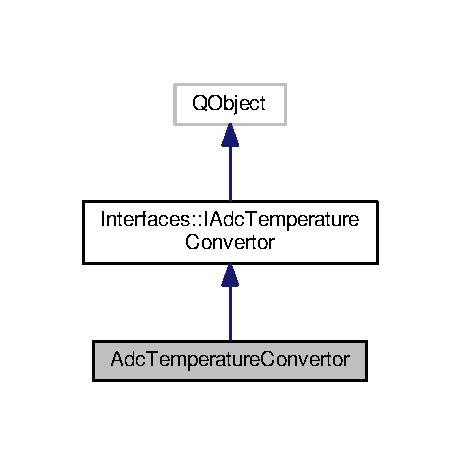
\includegraphics[width=221pt]{class_adc_temperature_convertor__inherit__graph}
\end{center}
\end{figure}


Collaboration diagram for Adc\+Temperature\+Convertor\+:\nopagebreak
\begin{figure}[H]
\begin{center}
\leavevmode
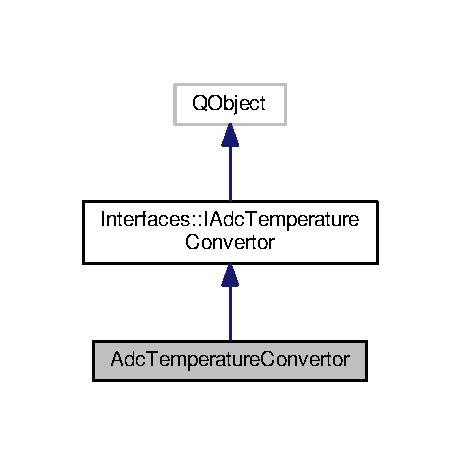
\includegraphics[width=221pt]{class_adc_temperature_convertor__coll__graph}
\end{center}
\end{figure}
\subsection*{Public Member Functions}
\begin{DoxyCompactItemize}
\item 
\mbox{\Hypertarget{class_adc_temperature_convertor_a3a78f66052068b96ace348d55e54d05c}\label{class_adc_temperature_convertor_a3a78f66052068b96ace348d55e54d05c}} 
\hyperlink{class_adc_temperature_convertor_a3a78f66052068b96ace348d55e54d05c}{Adc\+Temperature\+Convertor} ()
\begin{DoxyCompactList}\small\item\em Constructor. Call \hyperlink{class_adc_temperature_convertor_a5a19355f805554763e914e5b2216d5f6}{Set\+A\+D\+C2\+Temp\+Conversion\+Factors()} or \hyperlink{class_adc_temperature_convertor_affab0a66a3508e2eedd8bab3407ae80f}{Load\+Settings()} after class construction. \end{DoxyCompactList}\item 
double \hyperlink{class_adc_temperature_convertor_a3ee4549435400d9ed319fd5fdb83c97f}{A\+D\+C2\+T\+E\+MP} (uint adc)
\begin{DoxyCompactList}\small\item\em Convert A\+DC measurement to temperature (Celsius). \end{DoxyCompactList}\item 
uint \hyperlink{class_adc_temperature_convertor_ae82f374826a431c837bdf796c593775b}{T\+E\+M\+P2\+A\+DC} (double temp)
\begin{DoxyCompactList}\small\item\em Convert temperature in Celsius to A\+DC measurement. Imitates A\+DC saturation, i.\+e. returns 0 if value must be less than 0, and A\+D\+C\+\_\+\+M\+A\+X\+\_\+\+V\+A\+L\+UE if it must be more than A\+D\+C\+\_\+\+M\+A\+X\+\_\+\+V\+A\+L\+UE. \end{DoxyCompactList}\item 
void \hyperlink{class_adc_temperature_convertor_a5a19355f805554763e914e5b2216d5f6}{Set\+A\+D\+C2\+Temp\+Conversion\+Factors} (double a, double b)
\begin{DoxyCompactList}\small\item\em Call it to set A\+DC to Temperature conversion factors. Tc = a $\ast$ A\+DC + b, where Tc -\/ Temperature in Celsius, A\+DC -\/ A\+DC measurement. Reverse conversion factors (i.\+e. Temperature to A\+DC will be calculated automatically). \end{DoxyCompactList}\item 
void \hyperlink{class_adc_temperature_convertor_aeab56811467e8019731f1e2867a76671}{Get\+A\+D\+C2\+Temp\+Conversion\+Factors} (double $\ast$a, double $\ast$b)
\begin{DoxyCompactList}\small\item\em Returns temperature conversion factors (look \hyperlink{class_adc_temperature_convertor_a5a19355f805554763e914e5b2216d5f6}{Set\+A\+D\+C2\+Temp\+Conversion\+Factors()} for details). \end{DoxyCompactList}\item 
void \hyperlink{class_adc_temperature_convertor_affab0a66a3508e2eedd8bab3407ae80f}{Load\+Settings} (Q\+String filename)
\begin{DoxyCompactList}\small\item\em Load conversion settings from given file. \end{DoxyCompactList}\item 
void \hyperlink{class_adc_temperature_convertor_aa6935469c6bb9e2df9a21495d7e8b72a}{Save\+Settings} (Q\+String filename)
\begin{DoxyCompactList}\small\item\em Save conversion settings to given file. If file already exists it will be overwritten. \end{DoxyCompactList}\item 
void \hyperlink{class_adc_temperature_convertor_a56103443d7da4769339ddb685a0a8df0}{Set\+Description} (Q\+String descr)
\begin{DoxyCompactList}\small\item\em Set description of this instance (i.\+e. for this conversion settings). \end{DoxyCompactList}\item 
Q\+String \hyperlink{class_adc_temperature_convertor_ad82afdddbac46a95b6da44e769180d10}{Get\+Description} ()
\begin{DoxyCompactList}\small\item\em Get description of this instance (i.\+e. for this conversion settings). \end{DoxyCompactList}\item 
void \hyperlink{class_adc_temperature_convertor_aa06c19d0ac9f45d6f2f67718eda042ac}{Write\+A\+D\+C2\+Temperature\+Section} (Q\+Xml\+Stream\+Writer $\ast$writer)
\begin{DoxyCompactList}\small\item\em Writes A\+DC to temperature convertor settings section into given X\+ML writer. Use this method to embed A\+DC -\/$>$ Temperature settings into existing X\+ML file. \end{DoxyCompactList}\end{DoxyCompactItemize}


\subsection{Detailed Description}
Implementation of \hyperlink{class_interfaces_1_1_i_adc_temperature_convertor}{Interfaces\+::\+I\+Adc\+Temperature\+Convertor}. 

Definition at line 81 of file Adc\+Temperature\+Convertor.\+hpp.



\subsection{Member Function Documentation}
\mbox{\Hypertarget{class_adc_temperature_convertor_a3ee4549435400d9ed319fd5fdb83c97f}\label{class_adc_temperature_convertor_a3ee4549435400d9ed319fd5fdb83c97f}} 
\index{Adc\+Temperature\+Convertor@{Adc\+Temperature\+Convertor}!A\+D\+C2\+T\+E\+MP@{A\+D\+C2\+T\+E\+MP}}
\index{A\+D\+C2\+T\+E\+MP@{A\+D\+C2\+T\+E\+MP}!Adc\+Temperature\+Convertor@{Adc\+Temperature\+Convertor}}
\subsubsection{\texorpdfstring{A\+D\+C2\+T\+E\+M\+P()}{ADC2TEMP()}}
{\footnotesize\ttfamily double Adc\+Temperature\+Convertor\+::\+A\+D\+C2\+T\+E\+MP (\begin{DoxyParamCaption}\item[{uint}]{adc }\end{DoxyParamCaption})\hspace{0.3cm}{\ttfamily [virtual]}}



Convert A\+DC measurement to temperature (Celsius). 


\begin{DoxyParams}{Parameters}
{\em adc} & A\+DC measurement \\
\hline
\end{DoxyParams}
\begin{DoxyReturn}{Returns}
Temperature in Celsius 
\end{DoxyReturn}


Implements \hyperlink{class_interfaces_1_1_i_adc_temperature_convertor_aa6283c62cbbb012954b5e51d7a969385}{Interfaces\+::\+I\+Adc\+Temperature\+Convertor}.



Definition at line 32 of file Adc\+Temperature\+Convertor.\+cpp.

\mbox{\Hypertarget{class_adc_temperature_convertor_aeab56811467e8019731f1e2867a76671}\label{class_adc_temperature_convertor_aeab56811467e8019731f1e2867a76671}} 
\index{Adc\+Temperature\+Convertor@{Adc\+Temperature\+Convertor}!Get\+A\+D\+C2\+Temp\+Conversion\+Factors@{Get\+A\+D\+C2\+Temp\+Conversion\+Factors}}
\index{Get\+A\+D\+C2\+Temp\+Conversion\+Factors@{Get\+A\+D\+C2\+Temp\+Conversion\+Factors}!Adc\+Temperature\+Convertor@{Adc\+Temperature\+Convertor}}
\subsubsection{\texorpdfstring{Get\+A\+D\+C2\+Temp\+Conversion\+Factors()}{GetADC2TempConversionFactors()}}
{\footnotesize\ttfamily void Adc\+Temperature\+Convertor\+::\+Get\+A\+D\+C2\+Temp\+Conversion\+Factors (\begin{DoxyParamCaption}\item[{double $\ast$}]{a,  }\item[{double $\ast$}]{b }\end{DoxyParamCaption})\hspace{0.3cm}{\ttfamily [virtual]}}



Returns temperature conversion factors (look \hyperlink{class_adc_temperature_convertor_a5a19355f805554763e914e5b2216d5f6}{Set\+A\+D\+C2\+Temp\+Conversion\+Factors()} for details). 


\begin{DoxyParams}{Parameters}
{\em a} & Tc = a $\ast$ A\+DC + b \\
\hline
{\em b} & Tc = a $\ast$ A\+DC + b \\
\hline
\end{DoxyParams}


Implements \hyperlink{class_interfaces_1_1_i_adc_temperature_convertor_a61cff0aa0590906acfb18c9b789dceb2}{Interfaces\+::\+I\+Adc\+Temperature\+Convertor}.



Definition at line 58 of file Adc\+Temperature\+Convertor.\+cpp.

\mbox{\Hypertarget{class_adc_temperature_convertor_ad82afdddbac46a95b6da44e769180d10}\label{class_adc_temperature_convertor_ad82afdddbac46a95b6da44e769180d10}} 
\index{Adc\+Temperature\+Convertor@{Adc\+Temperature\+Convertor}!Get\+Description@{Get\+Description}}
\index{Get\+Description@{Get\+Description}!Adc\+Temperature\+Convertor@{Adc\+Temperature\+Convertor}}
\subsubsection{\texorpdfstring{Get\+Description()}{GetDescription()}}
{\footnotesize\ttfamily Q\+String Adc\+Temperature\+Convertor\+::\+Get\+Description (\begin{DoxyParamCaption}{ }\end{DoxyParamCaption})\hspace{0.3cm}{\ttfamily [virtual]}}



Get description of this instance (i.\+e. for this conversion settings). 

\begin{DoxyReturn}{Returns}
Description 
\end{DoxyReturn}


Implements \hyperlink{class_interfaces_1_1_i_adc_temperature_convertor_a2f3b59be793c3ed43e880ef12e9749bc}{Interfaces\+::\+I\+Adc\+Temperature\+Convertor}.



Definition at line 207 of file Adc\+Temperature\+Convertor.\+cpp.

\mbox{\Hypertarget{class_adc_temperature_convertor_affab0a66a3508e2eedd8bab3407ae80f}\label{class_adc_temperature_convertor_affab0a66a3508e2eedd8bab3407ae80f}} 
\index{Adc\+Temperature\+Convertor@{Adc\+Temperature\+Convertor}!Load\+Settings@{Load\+Settings}}
\index{Load\+Settings@{Load\+Settings}!Adc\+Temperature\+Convertor@{Adc\+Temperature\+Convertor}}
\subsubsection{\texorpdfstring{Load\+Settings()}{LoadSettings()}}
{\footnotesize\ttfamily void Adc\+Temperature\+Convertor\+::\+Load\+Settings (\begin{DoxyParamCaption}\item[{Q\+String}]{filename }\end{DoxyParamCaption})\hspace{0.3cm}{\ttfamily [virtual]}}



Load conversion settings from given file. 


\begin{DoxyParams}{Parameters}
{\em filename} & Full path to file with settings \\
\hline
\end{DoxyParams}


Implements \hyperlink{class_interfaces_1_1_i_adc_temperature_convertor_a9697a0319f82ebd1fc20f5e24d3b191c}{Interfaces\+::\+I\+Adc\+Temperature\+Convertor}.



Definition at line 65 of file Adc\+Temperature\+Convertor.\+cpp.

\mbox{\Hypertarget{class_adc_temperature_convertor_aa6935469c6bb9e2df9a21495d7e8b72a}\label{class_adc_temperature_convertor_aa6935469c6bb9e2df9a21495d7e8b72a}} 
\index{Adc\+Temperature\+Convertor@{Adc\+Temperature\+Convertor}!Save\+Settings@{Save\+Settings}}
\index{Save\+Settings@{Save\+Settings}!Adc\+Temperature\+Convertor@{Adc\+Temperature\+Convertor}}
\subsubsection{\texorpdfstring{Save\+Settings()}{SaveSettings()}}
{\footnotesize\ttfamily void Adc\+Temperature\+Convertor\+::\+Save\+Settings (\begin{DoxyParamCaption}\item[{Q\+String}]{filename }\end{DoxyParamCaption})\hspace{0.3cm}{\ttfamily [virtual]}}



Save conversion settings to given file. If file already exists it will be overwritten. 


\begin{DoxyParams}{Parameters}
{\em filename} & Full path to file where settings will be saved \\
\hline
\end{DoxyParams}


Implements \hyperlink{class_interfaces_1_1_i_adc_temperature_convertor_a6631e979e067ab78d3e5c337449876ac}{Interfaces\+::\+I\+Adc\+Temperature\+Convertor}.



Definition at line 172 of file Adc\+Temperature\+Convertor.\+cpp.

\mbox{\Hypertarget{class_adc_temperature_convertor_a5a19355f805554763e914e5b2216d5f6}\label{class_adc_temperature_convertor_a5a19355f805554763e914e5b2216d5f6}} 
\index{Adc\+Temperature\+Convertor@{Adc\+Temperature\+Convertor}!Set\+A\+D\+C2\+Temp\+Conversion\+Factors@{Set\+A\+D\+C2\+Temp\+Conversion\+Factors}}
\index{Set\+A\+D\+C2\+Temp\+Conversion\+Factors@{Set\+A\+D\+C2\+Temp\+Conversion\+Factors}!Adc\+Temperature\+Convertor@{Adc\+Temperature\+Convertor}}
\subsubsection{\texorpdfstring{Set\+A\+D\+C2\+Temp\+Conversion\+Factors()}{SetADC2TempConversionFactors()}}
{\footnotesize\ttfamily void Adc\+Temperature\+Convertor\+::\+Set\+A\+D\+C2\+Temp\+Conversion\+Factors (\begin{DoxyParamCaption}\item[{double}]{a,  }\item[{double}]{b }\end{DoxyParamCaption})\hspace{0.3cm}{\ttfamily [virtual]}}



Call it to set A\+DC to Temperature conversion factors. Tc = a $\ast$ A\+DC + b, where Tc -\/ Temperature in Celsius, A\+DC -\/ A\+DC measurement. Reverse conversion factors (i.\+e. Temperature to A\+DC will be calculated automatically). 


\begin{DoxyParams}{Parameters}
{\em a} & Tc = a $\ast$ A\+DC + b \\
\hline
{\em b} & Tc = a $\ast$ A\+DC + b \\
\hline
\end{DoxyParams}


Implements \hyperlink{class_interfaces_1_1_i_adc_temperature_convertor_a3e4c9204b3593bc434a041c7a69c430f}{Interfaces\+::\+I\+Adc\+Temperature\+Convertor}.



Definition at line 52 of file Adc\+Temperature\+Convertor.\+cpp.

\mbox{\Hypertarget{class_adc_temperature_convertor_a56103443d7da4769339ddb685a0a8df0}\label{class_adc_temperature_convertor_a56103443d7da4769339ddb685a0a8df0}} 
\index{Adc\+Temperature\+Convertor@{Adc\+Temperature\+Convertor}!Set\+Description@{Set\+Description}}
\index{Set\+Description@{Set\+Description}!Adc\+Temperature\+Convertor@{Adc\+Temperature\+Convertor}}
\subsubsection{\texorpdfstring{Set\+Description()}{SetDescription()}}
{\footnotesize\ttfamily void Adc\+Temperature\+Convertor\+::\+Set\+Description (\begin{DoxyParamCaption}\item[{Q\+String}]{descr }\end{DoxyParamCaption})\hspace{0.3cm}{\ttfamily [virtual]}}



Set description of this instance (i.\+e. for this conversion settings). 


\begin{DoxyParams}{Parameters}
{\em desct} & Description \\
\hline
\end{DoxyParams}


Implements \hyperlink{class_interfaces_1_1_i_adc_temperature_convertor_a65bbef2300e21c495d95305921ddb74b}{Interfaces\+::\+I\+Adc\+Temperature\+Convertor}.



Definition at line 202 of file Adc\+Temperature\+Convertor.\+cpp.

\mbox{\Hypertarget{class_adc_temperature_convertor_ae82f374826a431c837bdf796c593775b}\label{class_adc_temperature_convertor_ae82f374826a431c837bdf796c593775b}} 
\index{Adc\+Temperature\+Convertor@{Adc\+Temperature\+Convertor}!T\+E\+M\+P2\+A\+DC@{T\+E\+M\+P2\+A\+DC}}
\index{T\+E\+M\+P2\+A\+DC@{T\+E\+M\+P2\+A\+DC}!Adc\+Temperature\+Convertor@{Adc\+Temperature\+Convertor}}
\subsubsection{\texorpdfstring{T\+E\+M\+P2\+A\+D\+C()}{TEMP2ADC()}}
{\footnotesize\ttfamily uint Adc\+Temperature\+Convertor\+::\+T\+E\+M\+P2\+A\+DC (\begin{DoxyParamCaption}\item[{double}]{temp }\end{DoxyParamCaption})\hspace{0.3cm}{\ttfamily [virtual]}}



Convert temperature in Celsius to A\+DC measurement. Imitates A\+DC saturation, i.\+e. returns 0 if value must be less than 0, and A\+D\+C\+\_\+\+M\+A\+X\+\_\+\+V\+A\+L\+UE if it must be more than A\+D\+C\+\_\+\+M\+A\+X\+\_\+\+V\+A\+L\+UE. 


\begin{DoxyParams}{Parameters}
{\em temp} & Temperature in Celsius \\
\hline
\end{DoxyParams}
\begin{DoxyReturn}{Returns}
A\+DC measurement 
\end{DoxyReturn}


Implements \hyperlink{class_interfaces_1_1_i_adc_temperature_convertor_ab5d3453ecc41848b723a790fe7e01f79}{Interfaces\+::\+I\+Adc\+Temperature\+Convertor}.



Definition at line 37 of file Adc\+Temperature\+Convertor.\+cpp.

\mbox{\Hypertarget{class_adc_temperature_convertor_aa06c19d0ac9f45d6f2f67718eda042ac}\label{class_adc_temperature_convertor_aa06c19d0ac9f45d6f2f67718eda042ac}} 
\index{Adc\+Temperature\+Convertor@{Adc\+Temperature\+Convertor}!Write\+A\+D\+C2\+Temperature\+Section@{Write\+A\+D\+C2\+Temperature\+Section}}
\index{Write\+A\+D\+C2\+Temperature\+Section@{Write\+A\+D\+C2\+Temperature\+Section}!Adc\+Temperature\+Convertor@{Adc\+Temperature\+Convertor}}
\subsubsection{\texorpdfstring{Write\+A\+D\+C2\+Temperature\+Section()}{WriteADC2TemperatureSection()}}
{\footnotesize\ttfamily void Adc\+Temperature\+Convertor\+::\+Write\+A\+D\+C2\+Temperature\+Section (\begin{DoxyParamCaption}\item[{Q\+Xml\+Stream\+Writer $\ast$}]{writer }\end{DoxyParamCaption})\hspace{0.3cm}{\ttfamily [virtual]}}



Writes A\+DC to temperature convertor settings section into given X\+ML writer. Use this method to embed A\+DC -\/$>$ Temperature settings into existing X\+ML file. 


\begin{DoxyParams}{Parameters}
{\em writer} & Pointer to X\+ML writer. \\
\hline
\end{DoxyParams}


Implements \hyperlink{class_interfaces_1_1_i_adc_temperature_convertor_abc7ed5fdfeaed255af14930431b46ac1}{Interfaces\+::\+I\+Adc\+Temperature\+Convertor}.



Definition at line 191 of file Adc\+Temperature\+Convertor.\+cpp.



The documentation for this class was generated from the following files\+:\begin{DoxyCompactItemize}
\item 
Implementations/Adc\+Temperature\+Convertor.\+hpp\item 
Implementations/Adc\+Temperature\+Convertor.\+cpp\end{DoxyCompactItemize}

\hypertarget{class_interfaces_1_1_i_adc_temperature_convertor}{}\section{Interfaces\+:\+:I\+Adc\+Temperature\+Convertor Class Reference}
\label{class_interfaces_1_1_i_adc_temperature_convertor}\index{Interfaces\+::\+I\+Adc\+Temperature\+Convertor@{Interfaces\+::\+I\+Adc\+Temperature\+Convertor}}


Class, used to convert A\+DC values to Temperature and vice versa.  




{\ttfamily \#include $<$I\+Adc\+Temperature\+Convertor.\+hpp$>$}



Inheritance diagram for Interfaces\+:\+:I\+Adc\+Temperature\+Convertor\+:\nopagebreak
\begin{figure}[H]
\begin{center}
\leavevmode
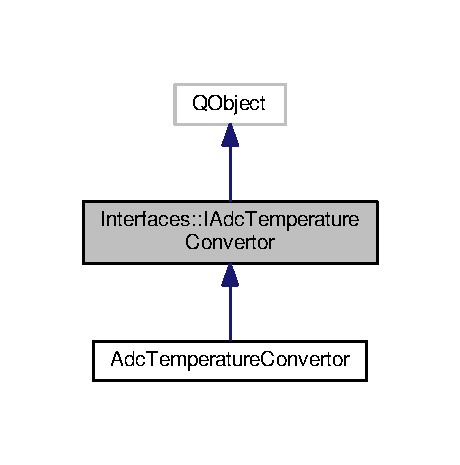
\includegraphics[width=221pt]{class_interfaces_1_1_i_adc_temperature_convertor__inherit__graph}
\end{center}
\end{figure}


Collaboration diagram for Interfaces\+:\+:I\+Adc\+Temperature\+Convertor\+:\nopagebreak
\begin{figure}[H]
\begin{center}
\leavevmode
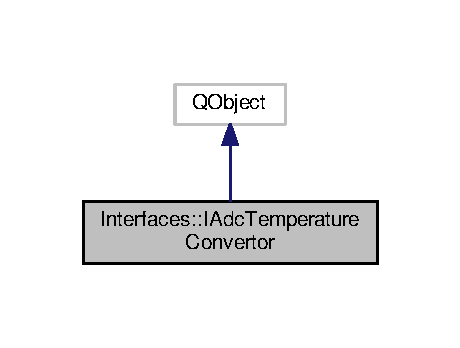
\includegraphics[width=221pt]{class_interfaces_1_1_i_adc_temperature_convertor__coll__graph}
\end{center}
\end{figure}
\subsection*{Public Member Functions}
\begin{DoxyCompactItemize}
\item 
virtual double \hyperlink{class_interfaces_1_1_i_adc_temperature_convertor_aa6283c62cbbb012954b5e51d7a969385}{A\+D\+C2\+T\+E\+MP} (uint adc)=0
\begin{DoxyCompactList}\small\item\em Convert A\+DC measurement to temperature (Celsius). \end{DoxyCompactList}\item 
virtual uint \hyperlink{class_interfaces_1_1_i_adc_temperature_convertor_ab5d3453ecc41848b723a790fe7e01f79}{T\+E\+M\+P2\+A\+DC} (double temp)=0
\begin{DoxyCompactList}\small\item\em Convert temperature in Celsius to A\+DC measurement. Imitates A\+DC saturation, i.\+e. returns 0 if value must be less than 0, and A\+D\+C\+\_\+\+M\+A\+X\+\_\+\+V\+A\+L\+UE if it must be more than A\+D\+C\+\_\+\+M\+A\+X\+\_\+\+V\+A\+L\+UE. \end{DoxyCompactList}\item 
virtual double \hyperlink{class_interfaces_1_1_i_adc_temperature_convertor_a70d62425963cadadd88db1d7028bf722}{Get\+Temp\+Delta} (uint adc1, uint adc2)=0
\begin{DoxyCompactList}\small\item\em Returns delta (in celsius) for two given A\+DC measurements. Delta is positive it adc2 means higher temperature then adc1. \end{DoxyCompactList}\item 
virtual void \hyperlink{class_interfaces_1_1_i_adc_temperature_convertor_a3e4c9204b3593bc434a041c7a69c430f}{Set\+A\+D\+C2\+Temp\+Conversion\+Factors} (double a, double b)=0
\begin{DoxyCompactList}\small\item\em Call it to set A\+DC to Temperature conversion factors. Tc = a $\ast$ A\+DC + b, where Tc -\/ Temperature in Celsius, A\+DC -\/ A\+DC measurement. Reverse conversion factors (i.\+e. Temperature to A\+DC will be calculated automatically). \end{DoxyCompactList}\item 
virtual void \hyperlink{class_interfaces_1_1_i_adc_temperature_convertor_a61cff0aa0590906acfb18c9b789dceb2}{Get\+A\+D\+C2\+Temp\+Conversion\+Factors} (double $\ast$a, double $\ast$b)=0
\begin{DoxyCompactList}\small\item\em Returns temperature conversion factors (look \hyperlink{class_interfaces_1_1_i_adc_temperature_convertor_a3e4c9204b3593bc434a041c7a69c430f}{Set\+A\+D\+C2\+Temp\+Conversion\+Factors()} for details). \end{DoxyCompactList}\item 
virtual void \hyperlink{class_interfaces_1_1_i_adc_temperature_convertor_a65bbef2300e21c495d95305921ddb74b}{Set\+Description} (Q\+String descr)=0
\begin{DoxyCompactList}\small\item\em Set description of this instance (i.\+e. for this conversion settings). \end{DoxyCompactList}\item 
virtual Q\+String \hyperlink{class_interfaces_1_1_i_adc_temperature_convertor_a2f3b59be793c3ed43e880ef12e9749bc}{Get\+Description} ()=0
\begin{DoxyCompactList}\small\item\em Get description of this instance (i.\+e. for this conversion settings). \end{DoxyCompactList}\item 
virtual bool \hyperlink{class_interfaces_1_1_i_adc_temperature_convertor_a3b1d84ea243b62a36238f16433668a23}{Load\+Settings} (Q\+String filename, Q\+String prefix)=0
\begin{DoxyCompactList}\small\item\em Load conversion settings from given file. File may contain only settings, or another data too. \end{DoxyCompactList}\item 
virtual void \hyperlink{class_interfaces_1_1_i_adc_temperature_convertor_a6631e979e067ab78d3e5c337449876ac}{Save\+Settings} (Q\+String filename)=0
\begin{DoxyCompactList}\small\item\em Save conversion settings to given file. If file already exists it will be overwritten. \end{DoxyCompactList}\item 
virtual void \hyperlink{class_interfaces_1_1_i_adc_temperature_convertor_abc7ed5fdfeaed255af14930431b46ac1}{Write\+A\+D\+C2\+Temperature\+Section} (Q\+Xml\+Stream\+Writer $\ast$writer)=0
\begin{DoxyCompactList}\small\item\em Writes A\+DC to temperature convertor settings section into given X\+ML writer. Use this method to embed A\+DC -\/$>$ Temperature settings into existing X\+ML file. \end{DoxyCompactList}\end{DoxyCompactItemize}


\subsection{Detailed Description}
Class, used to convert A\+DC values to Temperature and vice versa. 

Definition at line 43 of file I\+Adc\+Temperature\+Convertor.\+hpp.



\subsection{Member Function Documentation}
\mbox{\Hypertarget{class_interfaces_1_1_i_adc_temperature_convertor_aa6283c62cbbb012954b5e51d7a969385}\label{class_interfaces_1_1_i_adc_temperature_convertor_aa6283c62cbbb012954b5e51d7a969385}} 
\index{Interfaces\+::\+I\+Adc\+Temperature\+Convertor@{Interfaces\+::\+I\+Adc\+Temperature\+Convertor}!A\+D\+C2\+T\+E\+MP@{A\+D\+C2\+T\+E\+MP}}
\index{A\+D\+C2\+T\+E\+MP@{A\+D\+C2\+T\+E\+MP}!Interfaces\+::\+I\+Adc\+Temperature\+Convertor@{Interfaces\+::\+I\+Adc\+Temperature\+Convertor}}
\subsubsection{\texorpdfstring{A\+D\+C2\+T\+E\+M\+P()}{ADC2TEMP()}}
{\footnotesize\ttfamily virtual double Interfaces\+::\+I\+Adc\+Temperature\+Convertor\+::\+A\+D\+C2\+T\+E\+MP (\begin{DoxyParamCaption}\item[{uint}]{adc }\end{DoxyParamCaption})\hspace{0.3cm}{\ttfamily [pure virtual]}}



Convert A\+DC measurement to temperature (Celsius). 


\begin{DoxyParams}{Parameters}
{\em adc} & A\+DC measurement \\
\hline
\end{DoxyParams}
\begin{DoxyReturn}{Returns}
Temperature in Celsius 
\end{DoxyReturn}


Implemented in \hyperlink{class_adc_temperature_convertor_a3ee4549435400d9ed319fd5fdb83c97f}{Adc\+Temperature\+Convertor}.

\mbox{\Hypertarget{class_interfaces_1_1_i_adc_temperature_convertor_a61cff0aa0590906acfb18c9b789dceb2}\label{class_interfaces_1_1_i_adc_temperature_convertor_a61cff0aa0590906acfb18c9b789dceb2}} 
\index{Interfaces\+::\+I\+Adc\+Temperature\+Convertor@{Interfaces\+::\+I\+Adc\+Temperature\+Convertor}!Get\+A\+D\+C2\+Temp\+Conversion\+Factors@{Get\+A\+D\+C2\+Temp\+Conversion\+Factors}}
\index{Get\+A\+D\+C2\+Temp\+Conversion\+Factors@{Get\+A\+D\+C2\+Temp\+Conversion\+Factors}!Interfaces\+::\+I\+Adc\+Temperature\+Convertor@{Interfaces\+::\+I\+Adc\+Temperature\+Convertor}}
\subsubsection{\texorpdfstring{Get\+A\+D\+C2\+Temp\+Conversion\+Factors()}{GetADC2TempConversionFactors()}}
{\footnotesize\ttfamily virtual void Interfaces\+::\+I\+Adc\+Temperature\+Convertor\+::\+Get\+A\+D\+C2\+Temp\+Conversion\+Factors (\begin{DoxyParamCaption}\item[{double $\ast$}]{a,  }\item[{double $\ast$}]{b }\end{DoxyParamCaption})\hspace{0.3cm}{\ttfamily [pure virtual]}}



Returns temperature conversion factors (look \hyperlink{class_interfaces_1_1_i_adc_temperature_convertor_a3e4c9204b3593bc434a041c7a69c430f}{Set\+A\+D\+C2\+Temp\+Conversion\+Factors()} for details). 


\begin{DoxyParams}{Parameters}
{\em a} & Tc = a $\ast$ A\+DC + b \\
\hline
{\em b} & Tc = a $\ast$ A\+DC + b \\
\hline
\end{DoxyParams}


Implemented in \hyperlink{class_adc_temperature_convertor_af7c23effdc32aa35c14813fd334572f2}{Adc\+Temperature\+Convertor}.

\mbox{\Hypertarget{class_interfaces_1_1_i_adc_temperature_convertor_a2f3b59be793c3ed43e880ef12e9749bc}\label{class_interfaces_1_1_i_adc_temperature_convertor_a2f3b59be793c3ed43e880ef12e9749bc}} 
\index{Interfaces\+::\+I\+Adc\+Temperature\+Convertor@{Interfaces\+::\+I\+Adc\+Temperature\+Convertor}!Get\+Description@{Get\+Description}}
\index{Get\+Description@{Get\+Description}!Interfaces\+::\+I\+Adc\+Temperature\+Convertor@{Interfaces\+::\+I\+Adc\+Temperature\+Convertor}}
\subsubsection{\texorpdfstring{Get\+Description()}{GetDescription()}}
{\footnotesize\ttfamily virtual Q\+String Interfaces\+::\+I\+Adc\+Temperature\+Convertor\+::\+Get\+Description (\begin{DoxyParamCaption}{ }\end{DoxyParamCaption})\hspace{0.3cm}{\ttfamily [pure virtual]}}



Get description of this instance (i.\+e. for this conversion settings). 

\begin{DoxyReturn}{Returns}
Description 
\end{DoxyReturn}


Implemented in \hyperlink{class_adc_temperature_convertor_ad82afdddbac46a95b6da44e769180d10}{Adc\+Temperature\+Convertor}.

\mbox{\Hypertarget{class_interfaces_1_1_i_adc_temperature_convertor_a70d62425963cadadd88db1d7028bf722}\label{class_interfaces_1_1_i_adc_temperature_convertor_a70d62425963cadadd88db1d7028bf722}} 
\index{Interfaces\+::\+I\+Adc\+Temperature\+Convertor@{Interfaces\+::\+I\+Adc\+Temperature\+Convertor}!Get\+Temp\+Delta@{Get\+Temp\+Delta}}
\index{Get\+Temp\+Delta@{Get\+Temp\+Delta}!Interfaces\+::\+I\+Adc\+Temperature\+Convertor@{Interfaces\+::\+I\+Adc\+Temperature\+Convertor}}
\subsubsection{\texorpdfstring{Get\+Temp\+Delta()}{GetTempDelta()}}
{\footnotesize\ttfamily virtual double Interfaces\+::\+I\+Adc\+Temperature\+Convertor\+::\+Get\+Temp\+Delta (\begin{DoxyParamCaption}\item[{uint}]{adc1,  }\item[{uint}]{adc2 }\end{DoxyParamCaption})\hspace{0.3cm}{\ttfamily [pure virtual]}}



Returns delta (in celsius) for two given A\+DC measurements. Delta is positive it adc2 means higher temperature then adc1. 

\begin{DoxyReturn}{Returns}
Delta in celsius. 
\end{DoxyReturn}


Implemented in \hyperlink{class_adc_temperature_convertor_a6742f0177d4dcd1aab1087b5d7512146}{Adc\+Temperature\+Convertor}.

\mbox{\Hypertarget{class_interfaces_1_1_i_adc_temperature_convertor_a3b1d84ea243b62a36238f16433668a23}\label{class_interfaces_1_1_i_adc_temperature_convertor_a3b1d84ea243b62a36238f16433668a23}} 
\index{Interfaces\+::\+I\+Adc\+Temperature\+Convertor@{Interfaces\+::\+I\+Adc\+Temperature\+Convertor}!Load\+Settings@{Load\+Settings}}
\index{Load\+Settings@{Load\+Settings}!Interfaces\+::\+I\+Adc\+Temperature\+Convertor@{Interfaces\+::\+I\+Adc\+Temperature\+Convertor}}
\subsubsection{\texorpdfstring{Load\+Settings()}{LoadSettings()}}
{\footnotesize\ttfamily virtual bool Interfaces\+::\+I\+Adc\+Temperature\+Convertor\+::\+Load\+Settings (\begin{DoxyParamCaption}\item[{Q\+String}]{filename,  }\item[{Q\+String}]{prefix }\end{DoxyParamCaption})\hspace{0.3cm}{\ttfamily [pure virtual]}}



Load conversion settings from given file. File may contain only settings, or another data too. 


\begin{DoxyParams}{Parameters}
{\em filename} & Full path to file with settings. \\
\hline
{\em prefix} & Prefix for X\+ML data. I.\+e. set it to \char`\"{}\char`\"{} to load from root element, set it to \char`\"{}foo/bar/\char`\"{} to load from /foo/bar and so on. \\
\hline
\end{DoxyParams}
\begin{DoxyReturn}{Returns}
True if load successfull. 
\end{DoxyReturn}


Implemented in \hyperlink{class_adc_temperature_convertor_ac45f10e678aa2f9e25c5351dfd283de0}{Adc\+Temperature\+Convertor}.

\mbox{\Hypertarget{class_interfaces_1_1_i_adc_temperature_convertor_a6631e979e067ab78d3e5c337449876ac}\label{class_interfaces_1_1_i_adc_temperature_convertor_a6631e979e067ab78d3e5c337449876ac}} 
\index{Interfaces\+::\+I\+Adc\+Temperature\+Convertor@{Interfaces\+::\+I\+Adc\+Temperature\+Convertor}!Save\+Settings@{Save\+Settings}}
\index{Save\+Settings@{Save\+Settings}!Interfaces\+::\+I\+Adc\+Temperature\+Convertor@{Interfaces\+::\+I\+Adc\+Temperature\+Convertor}}
\subsubsection{\texorpdfstring{Save\+Settings()}{SaveSettings()}}
{\footnotesize\ttfamily virtual void Interfaces\+::\+I\+Adc\+Temperature\+Convertor\+::\+Save\+Settings (\begin{DoxyParamCaption}\item[{Q\+String}]{filename }\end{DoxyParamCaption})\hspace{0.3cm}{\ttfamily [pure virtual]}}



Save conversion settings to given file. If file already exists it will be overwritten. 


\begin{DoxyParams}{Parameters}
{\em filename} & Full path to file where settings will be saved \\
\hline
\end{DoxyParams}


Implemented in \hyperlink{class_adc_temperature_convertor_aa6935469c6bb9e2df9a21495d7e8b72a}{Adc\+Temperature\+Convertor}.

\mbox{\Hypertarget{class_interfaces_1_1_i_adc_temperature_convertor_a3e4c9204b3593bc434a041c7a69c430f}\label{class_interfaces_1_1_i_adc_temperature_convertor_a3e4c9204b3593bc434a041c7a69c430f}} 
\index{Interfaces\+::\+I\+Adc\+Temperature\+Convertor@{Interfaces\+::\+I\+Adc\+Temperature\+Convertor}!Set\+A\+D\+C2\+Temp\+Conversion\+Factors@{Set\+A\+D\+C2\+Temp\+Conversion\+Factors}}
\index{Set\+A\+D\+C2\+Temp\+Conversion\+Factors@{Set\+A\+D\+C2\+Temp\+Conversion\+Factors}!Interfaces\+::\+I\+Adc\+Temperature\+Convertor@{Interfaces\+::\+I\+Adc\+Temperature\+Convertor}}
\subsubsection{\texorpdfstring{Set\+A\+D\+C2\+Temp\+Conversion\+Factors()}{SetADC2TempConversionFactors()}}
{\footnotesize\ttfamily virtual void Interfaces\+::\+I\+Adc\+Temperature\+Convertor\+::\+Set\+A\+D\+C2\+Temp\+Conversion\+Factors (\begin{DoxyParamCaption}\item[{double}]{a,  }\item[{double}]{b }\end{DoxyParamCaption})\hspace{0.3cm}{\ttfamily [pure virtual]}}



Call it to set A\+DC to Temperature conversion factors. Tc = a $\ast$ A\+DC + b, where Tc -\/ Temperature in Celsius, A\+DC -\/ A\+DC measurement. Reverse conversion factors (i.\+e. Temperature to A\+DC will be calculated automatically). 


\begin{DoxyParams}{Parameters}
{\em a} & Tc = a $\ast$ A\+DC + b \\
\hline
{\em b} & Tc = a $\ast$ A\+DC + b \\
\hline
\end{DoxyParams}


Implemented in \hyperlink{class_adc_temperature_convertor_a4850843e55992608213cc9cf82d36830}{Adc\+Temperature\+Convertor}.

\mbox{\Hypertarget{class_interfaces_1_1_i_adc_temperature_convertor_a65bbef2300e21c495d95305921ddb74b}\label{class_interfaces_1_1_i_adc_temperature_convertor_a65bbef2300e21c495d95305921ddb74b}} 
\index{Interfaces\+::\+I\+Adc\+Temperature\+Convertor@{Interfaces\+::\+I\+Adc\+Temperature\+Convertor}!Set\+Description@{Set\+Description}}
\index{Set\+Description@{Set\+Description}!Interfaces\+::\+I\+Adc\+Temperature\+Convertor@{Interfaces\+::\+I\+Adc\+Temperature\+Convertor}}
\subsubsection{\texorpdfstring{Set\+Description()}{SetDescription()}}
{\footnotesize\ttfamily virtual void Interfaces\+::\+I\+Adc\+Temperature\+Convertor\+::\+Set\+Description (\begin{DoxyParamCaption}\item[{Q\+String}]{descr }\end{DoxyParamCaption})\hspace{0.3cm}{\ttfamily [pure virtual]}}



Set description of this instance (i.\+e. for this conversion settings). 


\begin{DoxyParams}{Parameters}
{\em desct} & Description \\
\hline
\end{DoxyParams}


Implemented in \hyperlink{class_adc_temperature_convertor_a56103443d7da4769339ddb685a0a8df0}{Adc\+Temperature\+Convertor}.

\mbox{\Hypertarget{class_interfaces_1_1_i_adc_temperature_convertor_ab5d3453ecc41848b723a790fe7e01f79}\label{class_interfaces_1_1_i_adc_temperature_convertor_ab5d3453ecc41848b723a790fe7e01f79}} 
\index{Interfaces\+::\+I\+Adc\+Temperature\+Convertor@{Interfaces\+::\+I\+Adc\+Temperature\+Convertor}!T\+E\+M\+P2\+A\+DC@{T\+E\+M\+P2\+A\+DC}}
\index{T\+E\+M\+P2\+A\+DC@{T\+E\+M\+P2\+A\+DC}!Interfaces\+::\+I\+Adc\+Temperature\+Convertor@{Interfaces\+::\+I\+Adc\+Temperature\+Convertor}}
\subsubsection{\texorpdfstring{T\+E\+M\+P2\+A\+D\+C()}{TEMP2ADC()}}
{\footnotesize\ttfamily virtual uint Interfaces\+::\+I\+Adc\+Temperature\+Convertor\+::\+T\+E\+M\+P2\+A\+DC (\begin{DoxyParamCaption}\item[{double}]{temp }\end{DoxyParamCaption})\hspace{0.3cm}{\ttfamily [pure virtual]}}



Convert temperature in Celsius to A\+DC measurement. Imitates A\+DC saturation, i.\+e. returns 0 if value must be less than 0, and A\+D\+C\+\_\+\+M\+A\+X\+\_\+\+V\+A\+L\+UE if it must be more than A\+D\+C\+\_\+\+M\+A\+X\+\_\+\+V\+A\+L\+UE. 


\begin{DoxyParams}{Parameters}
{\em temp} & Temperature in Celsius \\
\hline
\end{DoxyParams}
\begin{DoxyReturn}{Returns}
A\+DC measurement 
\end{DoxyReturn}


Implemented in \hyperlink{class_adc_temperature_convertor_ae82f374826a431c837bdf796c593775b}{Adc\+Temperature\+Convertor}.

\mbox{\Hypertarget{class_interfaces_1_1_i_adc_temperature_convertor_abc7ed5fdfeaed255af14930431b46ac1}\label{class_interfaces_1_1_i_adc_temperature_convertor_abc7ed5fdfeaed255af14930431b46ac1}} 
\index{Interfaces\+::\+I\+Adc\+Temperature\+Convertor@{Interfaces\+::\+I\+Adc\+Temperature\+Convertor}!Write\+A\+D\+C2\+Temperature\+Section@{Write\+A\+D\+C2\+Temperature\+Section}}
\index{Write\+A\+D\+C2\+Temperature\+Section@{Write\+A\+D\+C2\+Temperature\+Section}!Interfaces\+::\+I\+Adc\+Temperature\+Convertor@{Interfaces\+::\+I\+Adc\+Temperature\+Convertor}}
\subsubsection{\texorpdfstring{Write\+A\+D\+C2\+Temperature\+Section()}{WriteADC2TemperatureSection()}}
{\footnotesize\ttfamily virtual void Interfaces\+::\+I\+Adc\+Temperature\+Convertor\+::\+Write\+A\+D\+C2\+Temperature\+Section (\begin{DoxyParamCaption}\item[{Q\+Xml\+Stream\+Writer $\ast$}]{writer }\end{DoxyParamCaption})\hspace{0.3cm}{\ttfamily [pure virtual]}}



Writes A\+DC to temperature convertor settings section into given X\+ML writer. Use this method to embed A\+DC -\/$>$ Temperature settings into existing X\+ML file. 


\begin{DoxyParams}{Parameters}
{\em writer} & Pointer to X\+ML writer. \\
\hline
\end{DoxyParams}


Implemented in \hyperlink{class_adc_temperature_convertor_aa06c19d0ac9f45d6f2f67718eda042ac}{Adc\+Temperature\+Convertor}.



The documentation for this class was generated from the following file\+:\begin{DoxyCompactItemize}
\item 
Interfaces/I\+Adc\+Temperature\+Convertor.\+hpp\end{DoxyCompactItemize}

\hypertarget{class_fossa_1_1_q_simple_graph_1_1_interfaces_1_1_i_q_simple_graph}{}\section{Fossa\+:\+:Q\+Simple\+Graph\+:\+:Interfaces\+:\+:I\+Q\+Simple\+Graph Class Reference}
\label{class_fossa_1_1_q_simple_graph_1_1_interfaces_1_1_i_q_simple_graph}\index{Fossa\+::\+Q\+Simple\+Graph\+::\+Interfaces\+::\+I\+Q\+Simple\+Graph@{Fossa\+::\+Q\+Simple\+Graph\+::\+Interfaces\+::\+I\+Q\+Simple\+Graph}}


Main interface of \hyperlink{class_fossa_1_1_q_simple_graph_1_1_q_simple_graph}{Q\+Simple\+Graph}.  




{\ttfamily \#include $<$I\+Q\+Simple\+Graph.\+hpp$>$}



Inheritance diagram for Fossa\+:\+:Q\+Simple\+Graph\+:\+:Interfaces\+:\+:I\+Q\+Simple\+Graph\+:\nopagebreak
\begin{figure}[H]
\begin{center}
\leavevmode
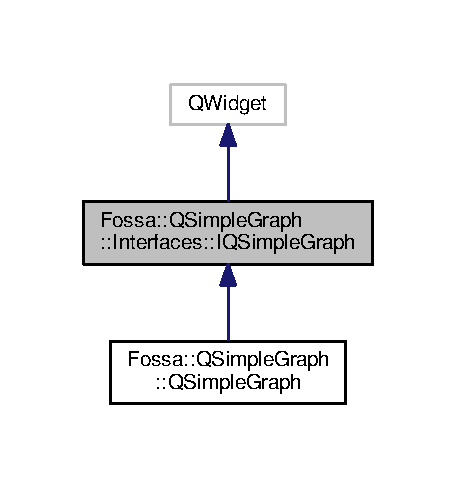
\includegraphics[width=219pt]{class_fossa_1_1_q_simple_graph_1_1_interfaces_1_1_i_q_simple_graph__inherit__graph}
\end{center}
\end{figure}


Collaboration diagram for Fossa\+:\+:Q\+Simple\+Graph\+:\+:Interfaces\+:\+:I\+Q\+Simple\+Graph\+:\nopagebreak
\begin{figure}[H]
\begin{center}
\leavevmode
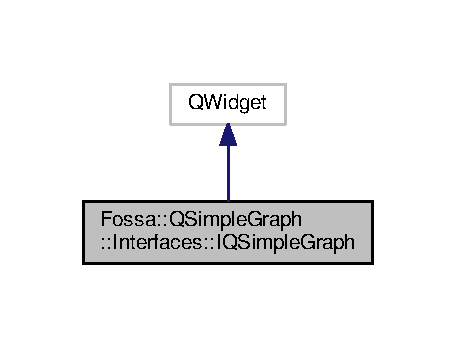
\includegraphics[width=219pt]{class_fossa_1_1_q_simple_graph_1_1_interfaces_1_1_i_q_simple_graph__coll__graph}
\end{center}
\end{figure}
\subsection*{Public Member Functions}
\begin{DoxyCompactItemize}
\item 
\hyperlink{class_fossa_1_1_q_simple_graph_1_1_interfaces_1_1_i_q_simple_graph_a7208e669127d3683d41329d110269e97}{I\+Q\+Simple\+Graph} (Q\+Widget $\ast$parent=0)
\begin{DoxyCompactList}\small\item\em Widget constructor. \end{DoxyCompactList}\item 
virtual void \hyperlink{class_fossa_1_1_q_simple_graph_1_1_interfaces_1_1_i_q_simple_graph_a4266725f87b306e572ad1ae37cfab4ef}{Set\+Min\+X\+Value} (double min\+Value)=0
\begin{DoxyCompactList}\small\item\em See Set\+Max\+X\+Value for details, it have completely the same behaviour. \end{DoxyCompactList}\item 
virtual void \hyperlink{class_fossa_1_1_q_simple_graph_1_1_interfaces_1_1_i_q_simple_graph_a04e7ec46c2be46257bef53c7bf978a2a}{Set\+Max\+X\+Value} (double max\+Value)=0
\begin{DoxyCompactList}\small\item\em Call it to set maximal value of X-\/axis. Please note, that if new point added to graph later, and point\textquotesingle{}s X coordinate exceeds maximal X value, then maximal X value will be increased, allowing graph to display such points. \end{DoxyCompactList}\item 
virtual void \hyperlink{class_fossa_1_1_q_simple_graph_1_1_interfaces_1_1_i_q_simple_graph_a3fdd1f6b538e2dfbf4a0140acd6b6e94}{Set\+Min\+Y\+Value} (double min\+Value)=0
\begin{DoxyCompactList}\small\item\em As Set\+Min\+X\+Value, but for Y-\/axis. \end{DoxyCompactList}\item 
virtual void \hyperlink{class_fossa_1_1_q_simple_graph_1_1_interfaces_1_1_i_q_simple_graph_a09e04c116810e79ca1663d2075477746}{Set\+Max\+Y\+Value} (double max\+Value)=0
\begin{DoxyCompactList}\small\item\em As Set\+Max\+X\+Value, but for Y-\/axis. \end{DoxyCompactList}\item 
virtual void \hyperlink{class_fossa_1_1_q_simple_graph_1_1_interfaces_1_1_i_q_simple_graph_adfca7d41a47790e8403507544468ba86}{Set\+X\+Axis\+Title} (Q\+String title)=0
\begin{DoxyCompactList}\small\item\em Set title of X-\/\+Axis. \end{DoxyCompactList}\item 
virtual void \hyperlink{class_fossa_1_1_q_simple_graph_1_1_interfaces_1_1_i_q_simple_graph_a606c07c40ed294cdd568de5488875af5}{Set\+Y\+Axis\+Title} (Q\+String title)=0
\begin{DoxyCompactList}\small\item\em As \hyperlink{class_fossa_1_1_q_simple_graph_1_1_interfaces_1_1_i_q_simple_graph_adfca7d41a47790e8403507544468ba86}{Set\+X\+Axis\+Title()}, but for Y-\/\+Axis. \end{DoxyCompactList}\item 
\mbox{\Hypertarget{class_fossa_1_1_q_simple_graph_1_1_interfaces_1_1_i_q_simple_graph_a2425d06ef062ee46b66574d40e9eb4f4}\label{class_fossa_1_1_q_simple_graph_1_1_interfaces_1_1_i_q_simple_graph_a2425d06ef062ee46b66574d40e9eb4f4}} 
virtual void \hyperlink{class_fossa_1_1_q_simple_graph_1_1_interfaces_1_1_i_q_simple_graph_a2425d06ef062ee46b66574d40e9eb4f4}{Clear\+All\+Points} ()=0
\begin{DoxyCompactList}\small\item\em Removes all points from graph. \end{DoxyCompactList}\item 
virtual void \hyperlink{class_fossa_1_1_q_simple_graph_1_1_interfaces_1_1_i_q_simple_graph_a5d43e4e0f06bedb1734e4240070fe229}{Add\+Point} (double X\+Val, double Y\+Val)=0
\begin{DoxyCompactList}\small\item\em Adds point with given X and Y value to graph. Points collection inside the graph must be self-\/ordered, so points can be added in arbitraty order. If point outside maximal and minimal values for graph, minimal and maximal values will be expanded to allow display all points. \end{DoxyCompactList}\end{DoxyCompactItemize}


\subsection{Detailed Description}
Main interface of \hyperlink{class_fossa_1_1_q_simple_graph_1_1_q_simple_graph}{Q\+Simple\+Graph}. 

Definition at line 25 of file I\+Q\+Simple\+Graph.\+hpp.



\subsection{Constructor \& Destructor Documentation}
\mbox{\Hypertarget{class_fossa_1_1_q_simple_graph_1_1_interfaces_1_1_i_q_simple_graph_a7208e669127d3683d41329d110269e97}\label{class_fossa_1_1_q_simple_graph_1_1_interfaces_1_1_i_q_simple_graph_a7208e669127d3683d41329d110269e97}} 
\index{Fossa\+::\+Q\+Simple\+Graph\+::\+Interfaces\+::\+I\+Q\+Simple\+Graph@{Fossa\+::\+Q\+Simple\+Graph\+::\+Interfaces\+::\+I\+Q\+Simple\+Graph}!I\+Q\+Simple\+Graph@{I\+Q\+Simple\+Graph}}
\index{I\+Q\+Simple\+Graph@{I\+Q\+Simple\+Graph}!Fossa\+::\+Q\+Simple\+Graph\+::\+Interfaces\+::\+I\+Q\+Simple\+Graph@{Fossa\+::\+Q\+Simple\+Graph\+::\+Interfaces\+::\+I\+Q\+Simple\+Graph}}
\subsubsection{\texorpdfstring{I\+Q\+Simple\+Graph()}{IQSimpleGraph()}}
{\footnotesize\ttfamily Fossa\+::\+Q\+Simple\+Graph\+::\+Interfaces\+::\+I\+Q\+Simple\+Graph\+::\+I\+Q\+Simple\+Graph (\begin{DoxyParamCaption}\item[{Q\+Widget $\ast$}]{parent = {\ttfamily 0} }\end{DoxyParamCaption})\hspace{0.3cm}{\ttfamily [inline]}}



Widget constructor. 


\begin{DoxyParams}{Parameters}
{\em parent} & Parent widget. \\
\hline
\end{DoxyParams}


Definition at line 36 of file I\+Q\+Simple\+Graph.\+hpp.



\subsection{Member Function Documentation}
\mbox{\Hypertarget{class_fossa_1_1_q_simple_graph_1_1_interfaces_1_1_i_q_simple_graph_a5d43e4e0f06bedb1734e4240070fe229}\label{class_fossa_1_1_q_simple_graph_1_1_interfaces_1_1_i_q_simple_graph_a5d43e4e0f06bedb1734e4240070fe229}} 
\index{Fossa\+::\+Q\+Simple\+Graph\+::\+Interfaces\+::\+I\+Q\+Simple\+Graph@{Fossa\+::\+Q\+Simple\+Graph\+::\+Interfaces\+::\+I\+Q\+Simple\+Graph}!Add\+Point@{Add\+Point}}
\index{Add\+Point@{Add\+Point}!Fossa\+::\+Q\+Simple\+Graph\+::\+Interfaces\+::\+I\+Q\+Simple\+Graph@{Fossa\+::\+Q\+Simple\+Graph\+::\+Interfaces\+::\+I\+Q\+Simple\+Graph}}
\subsubsection{\texorpdfstring{Add\+Point()}{AddPoint()}}
{\footnotesize\ttfamily virtual void Fossa\+::\+Q\+Simple\+Graph\+::\+Interfaces\+::\+I\+Q\+Simple\+Graph\+::\+Add\+Point (\begin{DoxyParamCaption}\item[{double}]{X\+Val,  }\item[{double}]{Y\+Val }\end{DoxyParamCaption})\hspace{0.3cm}{\ttfamily [pure virtual]}}



Adds point with given X and Y value to graph. Points collection inside the graph must be self-\/ordered, so points can be added in arbitraty order. If point outside maximal and minimal values for graph, minimal and maximal values will be expanded to allow display all points. 


\begin{DoxyParams}{Parameters}
{\em X\+Val} & X-\/axis value. \\
\hline
{\em Y\+Val} & Y-\/axis value. \\
\hline
\end{DoxyParams}


Implemented in \hyperlink{class_fossa_1_1_q_simple_graph_1_1_q_simple_graph_a39fdbd2aa624b7b086b5761308d8d49c}{Fossa\+::\+Q\+Simple\+Graph\+::\+Q\+Simple\+Graph}.

\mbox{\Hypertarget{class_fossa_1_1_q_simple_graph_1_1_interfaces_1_1_i_q_simple_graph_a04e7ec46c2be46257bef53c7bf978a2a}\label{class_fossa_1_1_q_simple_graph_1_1_interfaces_1_1_i_q_simple_graph_a04e7ec46c2be46257bef53c7bf978a2a}} 
\index{Fossa\+::\+Q\+Simple\+Graph\+::\+Interfaces\+::\+I\+Q\+Simple\+Graph@{Fossa\+::\+Q\+Simple\+Graph\+::\+Interfaces\+::\+I\+Q\+Simple\+Graph}!Set\+Max\+X\+Value@{Set\+Max\+X\+Value}}
\index{Set\+Max\+X\+Value@{Set\+Max\+X\+Value}!Fossa\+::\+Q\+Simple\+Graph\+::\+Interfaces\+::\+I\+Q\+Simple\+Graph@{Fossa\+::\+Q\+Simple\+Graph\+::\+Interfaces\+::\+I\+Q\+Simple\+Graph}}
\subsubsection{\texorpdfstring{Set\+Max\+X\+Value()}{SetMaxXValue()}}
{\footnotesize\ttfamily virtual void Fossa\+::\+Q\+Simple\+Graph\+::\+Interfaces\+::\+I\+Q\+Simple\+Graph\+::\+Set\+Max\+X\+Value (\begin{DoxyParamCaption}\item[{double}]{max\+Value }\end{DoxyParamCaption})\hspace{0.3cm}{\ttfamily [pure virtual]}}



Call it to set maximal value of X-\/axis. Please note, that if new point added to graph later, and point\textquotesingle{}s X coordinate exceeds maximal X value, then maximal X value will be increased, allowing graph to display such points. 


\begin{DoxyParams}{Parameters}
{\em max\+Value} & New maximal value. If it less then minimal X value, it will be set to minimal X value. \\
\hline
\end{DoxyParams}


Implemented in \hyperlink{class_fossa_1_1_q_simple_graph_1_1_q_simple_graph_a568a2dea4e0307b6888aaa048b4da97a}{Fossa\+::\+Q\+Simple\+Graph\+::\+Q\+Simple\+Graph}.

\mbox{\Hypertarget{class_fossa_1_1_q_simple_graph_1_1_interfaces_1_1_i_q_simple_graph_a09e04c116810e79ca1663d2075477746}\label{class_fossa_1_1_q_simple_graph_1_1_interfaces_1_1_i_q_simple_graph_a09e04c116810e79ca1663d2075477746}} 
\index{Fossa\+::\+Q\+Simple\+Graph\+::\+Interfaces\+::\+I\+Q\+Simple\+Graph@{Fossa\+::\+Q\+Simple\+Graph\+::\+Interfaces\+::\+I\+Q\+Simple\+Graph}!Set\+Max\+Y\+Value@{Set\+Max\+Y\+Value}}
\index{Set\+Max\+Y\+Value@{Set\+Max\+Y\+Value}!Fossa\+::\+Q\+Simple\+Graph\+::\+Interfaces\+::\+I\+Q\+Simple\+Graph@{Fossa\+::\+Q\+Simple\+Graph\+::\+Interfaces\+::\+I\+Q\+Simple\+Graph}}
\subsubsection{\texorpdfstring{Set\+Max\+Y\+Value()}{SetMaxYValue()}}
{\footnotesize\ttfamily virtual void Fossa\+::\+Q\+Simple\+Graph\+::\+Interfaces\+::\+I\+Q\+Simple\+Graph\+::\+Set\+Max\+Y\+Value (\begin{DoxyParamCaption}\item[{double}]{max\+Value }\end{DoxyParamCaption})\hspace{0.3cm}{\ttfamily [pure virtual]}}



As Set\+Max\+X\+Value, but for Y-\/axis. 


\begin{DoxyParams}{Parameters}
{\em max\+Value} & See Set\+Max\+X\+Value. \\
\hline
\end{DoxyParams}


Implemented in \hyperlink{class_fossa_1_1_q_simple_graph_1_1_q_simple_graph_a6cb6eee80dc489f300e32263833cf1cd}{Fossa\+::\+Q\+Simple\+Graph\+::\+Q\+Simple\+Graph}.

\mbox{\Hypertarget{class_fossa_1_1_q_simple_graph_1_1_interfaces_1_1_i_q_simple_graph_a4266725f87b306e572ad1ae37cfab4ef}\label{class_fossa_1_1_q_simple_graph_1_1_interfaces_1_1_i_q_simple_graph_a4266725f87b306e572ad1ae37cfab4ef}} 
\index{Fossa\+::\+Q\+Simple\+Graph\+::\+Interfaces\+::\+I\+Q\+Simple\+Graph@{Fossa\+::\+Q\+Simple\+Graph\+::\+Interfaces\+::\+I\+Q\+Simple\+Graph}!Set\+Min\+X\+Value@{Set\+Min\+X\+Value}}
\index{Set\+Min\+X\+Value@{Set\+Min\+X\+Value}!Fossa\+::\+Q\+Simple\+Graph\+::\+Interfaces\+::\+I\+Q\+Simple\+Graph@{Fossa\+::\+Q\+Simple\+Graph\+::\+Interfaces\+::\+I\+Q\+Simple\+Graph}}
\subsubsection{\texorpdfstring{Set\+Min\+X\+Value()}{SetMinXValue()}}
{\footnotesize\ttfamily virtual void Fossa\+::\+Q\+Simple\+Graph\+::\+Interfaces\+::\+I\+Q\+Simple\+Graph\+::\+Set\+Min\+X\+Value (\begin{DoxyParamCaption}\item[{double}]{min\+Value }\end{DoxyParamCaption})\hspace{0.3cm}{\ttfamily [pure virtual]}}



See Set\+Max\+X\+Value for details, it have completely the same behaviour. 


\begin{DoxyParams}{Parameters}
{\em min\+Value} & New minimal value. If it greater then maximal X value, it will be set to maximal X value. \\
\hline
\end{DoxyParams}


Implemented in \hyperlink{class_fossa_1_1_q_simple_graph_1_1_q_simple_graph_a0eef21e58d8c85f6083d73857f871639}{Fossa\+::\+Q\+Simple\+Graph\+::\+Q\+Simple\+Graph}.

\mbox{\Hypertarget{class_fossa_1_1_q_simple_graph_1_1_interfaces_1_1_i_q_simple_graph_a3fdd1f6b538e2dfbf4a0140acd6b6e94}\label{class_fossa_1_1_q_simple_graph_1_1_interfaces_1_1_i_q_simple_graph_a3fdd1f6b538e2dfbf4a0140acd6b6e94}} 
\index{Fossa\+::\+Q\+Simple\+Graph\+::\+Interfaces\+::\+I\+Q\+Simple\+Graph@{Fossa\+::\+Q\+Simple\+Graph\+::\+Interfaces\+::\+I\+Q\+Simple\+Graph}!Set\+Min\+Y\+Value@{Set\+Min\+Y\+Value}}
\index{Set\+Min\+Y\+Value@{Set\+Min\+Y\+Value}!Fossa\+::\+Q\+Simple\+Graph\+::\+Interfaces\+::\+I\+Q\+Simple\+Graph@{Fossa\+::\+Q\+Simple\+Graph\+::\+Interfaces\+::\+I\+Q\+Simple\+Graph}}
\subsubsection{\texorpdfstring{Set\+Min\+Y\+Value()}{SetMinYValue()}}
{\footnotesize\ttfamily virtual void Fossa\+::\+Q\+Simple\+Graph\+::\+Interfaces\+::\+I\+Q\+Simple\+Graph\+::\+Set\+Min\+Y\+Value (\begin{DoxyParamCaption}\item[{double}]{min\+Value }\end{DoxyParamCaption})\hspace{0.3cm}{\ttfamily [pure virtual]}}



As Set\+Min\+X\+Value, but for Y-\/axis. 


\begin{DoxyParams}{Parameters}
{\em min\+Value} & See Set\+Min\+X\+Value. \\
\hline
\end{DoxyParams}


Implemented in \hyperlink{class_fossa_1_1_q_simple_graph_1_1_q_simple_graph_a8bf9aac5856a659eb89abffca7750df0}{Fossa\+::\+Q\+Simple\+Graph\+::\+Q\+Simple\+Graph}.

\mbox{\Hypertarget{class_fossa_1_1_q_simple_graph_1_1_interfaces_1_1_i_q_simple_graph_adfca7d41a47790e8403507544468ba86}\label{class_fossa_1_1_q_simple_graph_1_1_interfaces_1_1_i_q_simple_graph_adfca7d41a47790e8403507544468ba86}} 
\index{Fossa\+::\+Q\+Simple\+Graph\+::\+Interfaces\+::\+I\+Q\+Simple\+Graph@{Fossa\+::\+Q\+Simple\+Graph\+::\+Interfaces\+::\+I\+Q\+Simple\+Graph}!Set\+X\+Axis\+Title@{Set\+X\+Axis\+Title}}
\index{Set\+X\+Axis\+Title@{Set\+X\+Axis\+Title}!Fossa\+::\+Q\+Simple\+Graph\+::\+Interfaces\+::\+I\+Q\+Simple\+Graph@{Fossa\+::\+Q\+Simple\+Graph\+::\+Interfaces\+::\+I\+Q\+Simple\+Graph}}
\subsubsection{\texorpdfstring{Set\+X\+Axis\+Title()}{SetXAxisTitle()}}
{\footnotesize\ttfamily virtual void Fossa\+::\+Q\+Simple\+Graph\+::\+Interfaces\+::\+I\+Q\+Simple\+Graph\+::\+Set\+X\+Axis\+Title (\begin{DoxyParamCaption}\item[{Q\+String}]{title }\end{DoxyParamCaption})\hspace{0.3cm}{\ttfamily [pure virtual]}}



Set title of X-\/\+Axis. 


\begin{DoxyParams}{Parameters}
{\em title} & Title. \\
\hline
\end{DoxyParams}


Implemented in \hyperlink{class_fossa_1_1_q_simple_graph_1_1_q_simple_graph_a7579da572b54d43ccec3d2bd572b6cfa}{Fossa\+::\+Q\+Simple\+Graph\+::\+Q\+Simple\+Graph}.

\mbox{\Hypertarget{class_fossa_1_1_q_simple_graph_1_1_interfaces_1_1_i_q_simple_graph_a606c07c40ed294cdd568de5488875af5}\label{class_fossa_1_1_q_simple_graph_1_1_interfaces_1_1_i_q_simple_graph_a606c07c40ed294cdd568de5488875af5}} 
\index{Fossa\+::\+Q\+Simple\+Graph\+::\+Interfaces\+::\+I\+Q\+Simple\+Graph@{Fossa\+::\+Q\+Simple\+Graph\+::\+Interfaces\+::\+I\+Q\+Simple\+Graph}!Set\+Y\+Axis\+Title@{Set\+Y\+Axis\+Title}}
\index{Set\+Y\+Axis\+Title@{Set\+Y\+Axis\+Title}!Fossa\+::\+Q\+Simple\+Graph\+::\+Interfaces\+::\+I\+Q\+Simple\+Graph@{Fossa\+::\+Q\+Simple\+Graph\+::\+Interfaces\+::\+I\+Q\+Simple\+Graph}}
\subsubsection{\texorpdfstring{Set\+Y\+Axis\+Title()}{SetYAxisTitle()}}
{\footnotesize\ttfamily virtual void Fossa\+::\+Q\+Simple\+Graph\+::\+Interfaces\+::\+I\+Q\+Simple\+Graph\+::\+Set\+Y\+Axis\+Title (\begin{DoxyParamCaption}\item[{Q\+String}]{title }\end{DoxyParamCaption})\hspace{0.3cm}{\ttfamily [pure virtual]}}



As \hyperlink{class_fossa_1_1_q_simple_graph_1_1_interfaces_1_1_i_q_simple_graph_adfca7d41a47790e8403507544468ba86}{Set\+X\+Axis\+Title()}, but for Y-\/\+Axis. 


\begin{DoxyParams}{Parameters}
{\em title} & See \hyperlink{class_fossa_1_1_q_simple_graph_1_1_interfaces_1_1_i_q_simple_graph_adfca7d41a47790e8403507544468ba86}{Set\+X\+Axis\+Title()}. \\
\hline
\end{DoxyParams}


Implemented in \hyperlink{class_fossa_1_1_q_simple_graph_1_1_q_simple_graph_a41c9e9d34744f6e6550ca97dc0d2f488}{Fossa\+::\+Q\+Simple\+Graph\+::\+Q\+Simple\+Graph}.



The documentation for this class was generated from the following file\+:\begin{DoxyCompactItemize}
\item 
Fossas\+Simple\+Graph/\+Interfaces/I\+Q\+Simple\+Graph.\+hpp\end{DoxyCompactItemize}

\hypertarget{class_interfaces_1_1_i_settings_generator}{}\section{Interfaces\+:\+:I\+Settings\+Generator Class Reference}
\label{class_interfaces_1_1_i_settings_generator}\index{Interfaces\+::\+I\+Settings\+Generator@{Interfaces\+::\+I\+Settings\+Generator}}


Class, containing all settings steps. It being used to generate settings table, which will be converted to E\+E\+P\+R\+OM data.  




{\ttfamily \#include $<$I\+Settings\+Generator.\+hpp$>$}



Inheritance diagram for Interfaces\+:\+:I\+Settings\+Generator\+:\nopagebreak
\begin{figure}[H]
\begin{center}
\leavevmode
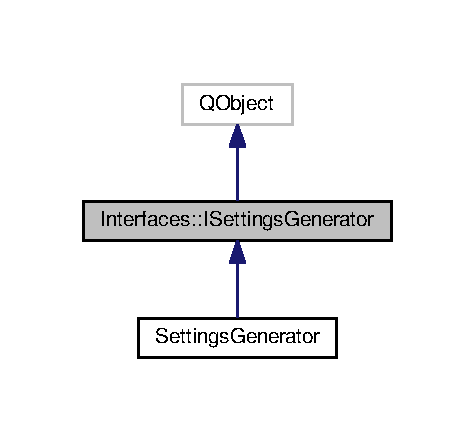
\includegraphics[width=228pt]{class_interfaces_1_1_i_settings_generator__inherit__graph}
\end{center}
\end{figure}


Collaboration diagram for Interfaces\+:\+:I\+Settings\+Generator\+:\nopagebreak
\begin{figure}[H]
\begin{center}
\leavevmode
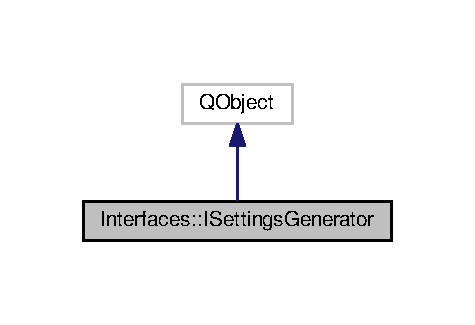
\includegraphics[width=228pt]{class_interfaces_1_1_i_settings_generator__coll__graph}
\end{center}
\end{figure}
\subsection*{Public Member Functions}
\begin{DoxyCompactItemize}
\item 
virtual void \hyperlink{class_interfaces_1_1_i_settings_generator_a4aa0307e906c003012aad75101072c65}{Initialize\+Steps\+List} (uint steps\+\_\+number)=0
\begin{DoxyCompactList}\small\item\em Call this method to initialize steps list. It must be called before any other methods. Implementation must be ready to provide the instance of \hyperlink{class_interfaces_1_1_i_adc_temperature_convertor}{I\+Adc\+Temperature\+Convertor} to steps. \end{DoxyCompactList}\item 
virtual void \hyperlink{class_interfaces_1_1_i_settings_generator_a8b60ba05790994db0303b251f655e95d}{Set\+Base\+Temperature} (double btemp)=0
\begin{DoxyCompactList}\small\item\em Set\+Base\+Temperature -\/ Call it to set base temperature (in Celsius). Please note, that all steps will be recalculated afterwards. \end{DoxyCompactList}\item 
virtual double \hyperlink{class_interfaces_1_1_i_settings_generator_a9cc36185b446f21e09a0e5633f39a1c5}{Get\+Base\+Temperature} ()=0
\begin{DoxyCompactList}\small\item\em Get\+Base\+Temperature -\/ Call it to get base temperature (in Celsius). Please note, that base temperature returned by this method M\+AY D\+I\+F\+F\+ER from that, what was set by \hyperlink{class_interfaces_1_1_i_settings_generator_a8b60ba05790994db0303b251f655e95d}{Set\+Base\+Temperature()}. It is because implementation may store A\+DC value rather than temperature. \end{DoxyCompactList}\item 
virtual uint \hyperlink{class_interfaces_1_1_i_settings_generator_a1000ff41c6eecdb55a46c859ca0ebe67}{Get\+Base\+Temperature\+A\+DC} ()=0
\begin{DoxyCompactList}\small\item\em Get\+Base\+Temperature\+A\+DC Like \hyperlink{class_interfaces_1_1_i_settings_generator_a9cc36185b446f21e09a0e5633f39a1c5}{Get\+Base\+Temperature()}, but returns A\+DC code for it. \end{DoxyCompactList}\item 
virtual void \hyperlink{class_interfaces_1_1_i_settings_generator_a4caf07447d0930440d9f21318892244c}{Set\+Base\+R\+PM} (uint base\+\_\+rpm)=0
\begin{DoxyCompactList}\small\item\em Set\+Base\+Rpm Call this method to set base R\+PM. Base R\+PM -\/ is a R\+PM at base temperature. Please note, that all steps will be recalculated afterwards. \end{DoxyCompactList}\item 
virtual uint \hyperlink{class_interfaces_1_1_i_settings_generator_ad088253da57b2ee0b94fe6fd1fb2dfdd}{Get\+Base\+R\+PM} ()=0
\begin{DoxyCompactList}\small\item\em Get\+Base\+R\+PM -\/ Returns base R\+PM level. See \hyperlink{class_interfaces_1_1_i_settings_generator_a4caf07447d0930440d9f21318892244c}{Set\+Base\+R\+P\+M()} for details. \end{DoxyCompactList}\item 
\mbox{\Hypertarget{class_interfaces_1_1_i_settings_generator_a7788522bb5d25bfd8b8af430512ec5f5}\label{class_interfaces_1_1_i_settings_generator_a7788522bb5d25bfd8b8af430512ec5f5}} 
virtual void \hyperlink{class_interfaces_1_1_i_settings_generator_a7788522bb5d25bfd8b8af430512ec5f5}{Calculate\+Steps} ()=0
\begin{DoxyCompactList}\small\item\em Calculate\+Steps Call this method to recalculate step A\+DC levels and R\+P\+Ms. \end{DoxyCompactList}\item 
virtual \hyperlink{class_interfaces_1_1_i_settings_step}{Interfaces\+::\+I\+Settings\+Step} $\ast$ \hyperlink{class_interfaces_1_1_i_settings_generator_af1b65a18c3ade3235715ae2e9cdbcfe0}{Get\+Step\+Ptr} (uint step)=0
\begin{DoxyCompactList}\small\item\em Returns pointer to step with given number to allow manipulations with step. Don\textquotesingle{}t forget to call \hyperlink{class_interfaces_1_1_i_settings_generator_a7788522bb5d25bfd8b8af430512ec5f5}{Calculate\+Steps()} after making any changes. \end{DoxyCompactList}\end{DoxyCompactItemize}


\subsection{Detailed Description}
Class, containing all settings steps. It being used to generate settings table, which will be converted to E\+E\+P\+R\+OM data. 

Definition at line 32 of file I\+Settings\+Generator.\+hpp.



\subsection{Member Function Documentation}
\mbox{\Hypertarget{class_interfaces_1_1_i_settings_generator_ad088253da57b2ee0b94fe6fd1fb2dfdd}\label{class_interfaces_1_1_i_settings_generator_ad088253da57b2ee0b94fe6fd1fb2dfdd}} 
\index{Interfaces\+::\+I\+Settings\+Generator@{Interfaces\+::\+I\+Settings\+Generator}!Get\+Base\+R\+PM@{Get\+Base\+R\+PM}}
\index{Get\+Base\+R\+PM@{Get\+Base\+R\+PM}!Interfaces\+::\+I\+Settings\+Generator@{Interfaces\+::\+I\+Settings\+Generator}}
\subsubsection{\texorpdfstring{Get\+Base\+R\+P\+M()}{GetBaseRPM()}}
{\footnotesize\ttfamily virtual uint Interfaces\+::\+I\+Settings\+Generator\+::\+Get\+Base\+R\+PM (\begin{DoxyParamCaption}{ }\end{DoxyParamCaption})\hspace{0.3cm}{\ttfamily [pure virtual]}}



Get\+Base\+R\+PM -\/ Returns base R\+PM level. See \hyperlink{class_interfaces_1_1_i_settings_generator_a4caf07447d0930440d9f21318892244c}{Set\+Base\+R\+P\+M()} for details. 

\begin{DoxyReturn}{Returns}
Base R\+PM level. 
\end{DoxyReturn}


Implemented in \hyperlink{class_settings_generator_a99bbe6e67e638ccc7bf6b21b3bc36135}{Settings\+Generator}.

\mbox{\Hypertarget{class_interfaces_1_1_i_settings_generator_a9cc36185b446f21e09a0e5633f39a1c5}\label{class_interfaces_1_1_i_settings_generator_a9cc36185b446f21e09a0e5633f39a1c5}} 
\index{Interfaces\+::\+I\+Settings\+Generator@{Interfaces\+::\+I\+Settings\+Generator}!Get\+Base\+Temperature@{Get\+Base\+Temperature}}
\index{Get\+Base\+Temperature@{Get\+Base\+Temperature}!Interfaces\+::\+I\+Settings\+Generator@{Interfaces\+::\+I\+Settings\+Generator}}
\subsubsection{\texorpdfstring{Get\+Base\+Temperature()}{GetBaseTemperature()}}
{\footnotesize\ttfamily virtual double Interfaces\+::\+I\+Settings\+Generator\+::\+Get\+Base\+Temperature (\begin{DoxyParamCaption}{ }\end{DoxyParamCaption})\hspace{0.3cm}{\ttfamily [pure virtual]}}



Get\+Base\+Temperature -\/ Call it to get base temperature (in Celsius). Please note, that base temperature returned by this method M\+AY D\+I\+F\+F\+ER from that, what was set by \hyperlink{class_interfaces_1_1_i_settings_generator_a8b60ba05790994db0303b251f655e95d}{Set\+Base\+Temperature()}. It is because implementation may store A\+DC value rather than temperature. 

\begin{DoxyReturn}{Returns}
Base temperature in Celsius 
\end{DoxyReturn}


Implemented in \hyperlink{class_settings_generator_a80b1ff8060a16d149989d98a88ab253e}{Settings\+Generator}.

\mbox{\Hypertarget{class_interfaces_1_1_i_settings_generator_a1000ff41c6eecdb55a46c859ca0ebe67}\label{class_interfaces_1_1_i_settings_generator_a1000ff41c6eecdb55a46c859ca0ebe67}} 
\index{Interfaces\+::\+I\+Settings\+Generator@{Interfaces\+::\+I\+Settings\+Generator}!Get\+Base\+Temperature\+A\+DC@{Get\+Base\+Temperature\+A\+DC}}
\index{Get\+Base\+Temperature\+A\+DC@{Get\+Base\+Temperature\+A\+DC}!Interfaces\+::\+I\+Settings\+Generator@{Interfaces\+::\+I\+Settings\+Generator}}
\subsubsection{\texorpdfstring{Get\+Base\+Temperature\+A\+D\+C()}{GetBaseTemperatureADC()}}
{\footnotesize\ttfamily virtual uint Interfaces\+::\+I\+Settings\+Generator\+::\+Get\+Base\+Temperature\+A\+DC (\begin{DoxyParamCaption}{ }\end{DoxyParamCaption})\hspace{0.3cm}{\ttfamily [pure virtual]}}



Get\+Base\+Temperature\+A\+DC Like \hyperlink{class_interfaces_1_1_i_settings_generator_a9cc36185b446f21e09a0e5633f39a1c5}{Get\+Base\+Temperature()}, but returns A\+DC code for it. 

\begin{DoxyReturn}{Returns}
A\+DC code for current base temperature. 
\end{DoxyReturn}


Implemented in \hyperlink{class_settings_generator_a5f3f78597f001c127b89f6447a46df09}{Settings\+Generator}.

\mbox{\Hypertarget{class_interfaces_1_1_i_settings_generator_af1b65a18c3ade3235715ae2e9cdbcfe0}\label{class_interfaces_1_1_i_settings_generator_af1b65a18c3ade3235715ae2e9cdbcfe0}} 
\index{Interfaces\+::\+I\+Settings\+Generator@{Interfaces\+::\+I\+Settings\+Generator}!Get\+Step\+Ptr@{Get\+Step\+Ptr}}
\index{Get\+Step\+Ptr@{Get\+Step\+Ptr}!Interfaces\+::\+I\+Settings\+Generator@{Interfaces\+::\+I\+Settings\+Generator}}
\subsubsection{\texorpdfstring{Get\+Step\+Ptr()}{GetStepPtr()}}
{\footnotesize\ttfamily virtual \hyperlink{class_interfaces_1_1_i_settings_step}{Interfaces\+::\+I\+Settings\+Step}$\ast$ Interfaces\+::\+I\+Settings\+Generator\+::\+Get\+Step\+Ptr (\begin{DoxyParamCaption}\item[{uint}]{step }\end{DoxyParamCaption})\hspace{0.3cm}{\ttfamily [pure virtual]}}



Returns pointer to step with given number to allow manipulations with step. Don\textquotesingle{}t forget to call \hyperlink{class_interfaces_1_1_i_settings_generator_a7788522bb5d25bfd8b8af430512ec5f5}{Calculate\+Steps()} after making any changes. 


\begin{DoxyParams}{Parameters}
{\em step} & Step number \\
\hline
\end{DoxyParams}
\begin{DoxyReturn}{Returns}
Pointer to step 
\end{DoxyReturn}


Implemented in \hyperlink{class_settings_generator_a37f4175a0ed24853b2f187f15505086b}{Settings\+Generator}.

\mbox{\Hypertarget{class_interfaces_1_1_i_settings_generator_a4aa0307e906c003012aad75101072c65}\label{class_interfaces_1_1_i_settings_generator_a4aa0307e906c003012aad75101072c65}} 
\index{Interfaces\+::\+I\+Settings\+Generator@{Interfaces\+::\+I\+Settings\+Generator}!Initialize\+Steps\+List@{Initialize\+Steps\+List}}
\index{Initialize\+Steps\+List@{Initialize\+Steps\+List}!Interfaces\+::\+I\+Settings\+Generator@{Interfaces\+::\+I\+Settings\+Generator}}
\subsubsection{\texorpdfstring{Initialize\+Steps\+List()}{InitializeStepsList()}}
{\footnotesize\ttfamily virtual void Interfaces\+::\+I\+Settings\+Generator\+::\+Initialize\+Steps\+List (\begin{DoxyParamCaption}\item[{uint}]{steps\+\_\+number }\end{DoxyParamCaption})\hspace{0.3cm}{\ttfamily [pure virtual]}}



Call this method to initialize steps list. It must be called before any other methods. Implementation must be ready to provide the instance of \hyperlink{class_interfaces_1_1_i_adc_temperature_convertor}{I\+Adc\+Temperature\+Convertor} to steps. 


\begin{DoxyParams}{Parameters}
{\em steps\+\_\+number} & How many steps we have \\
\hline
\end{DoxyParams}


Implemented in \hyperlink{class_settings_generator_a84b81d11cb5f83d4066e73a03acfc143}{Settings\+Generator}.

\mbox{\Hypertarget{class_interfaces_1_1_i_settings_generator_a4caf07447d0930440d9f21318892244c}\label{class_interfaces_1_1_i_settings_generator_a4caf07447d0930440d9f21318892244c}} 
\index{Interfaces\+::\+I\+Settings\+Generator@{Interfaces\+::\+I\+Settings\+Generator}!Set\+Base\+R\+PM@{Set\+Base\+R\+PM}}
\index{Set\+Base\+R\+PM@{Set\+Base\+R\+PM}!Interfaces\+::\+I\+Settings\+Generator@{Interfaces\+::\+I\+Settings\+Generator}}
\subsubsection{\texorpdfstring{Set\+Base\+R\+P\+M()}{SetBaseRPM()}}
{\footnotesize\ttfamily virtual void Interfaces\+::\+I\+Settings\+Generator\+::\+Set\+Base\+R\+PM (\begin{DoxyParamCaption}\item[{uint}]{base\+\_\+rpm }\end{DoxyParamCaption})\hspace{0.3cm}{\ttfamily [pure virtual]}}



Set\+Base\+Rpm Call this method to set base R\+PM. Base R\+PM -\/ is a R\+PM at base temperature. Please note, that all steps will be recalculated afterwards. 


\begin{DoxyParams}{Parameters}
{\em base\+\_\+rpm} & -\/ Base R\+PM value. 0x00 -\/ cooler is stopped. 0x01 -\/ minimal possible R\+PM. 0x100 -\/ maximal possible R\+PM. \\
\hline
\end{DoxyParams}


Implemented in \hyperlink{class_settings_generator_a1c1960b9021f7081b4c42c4d7c0eda34}{Settings\+Generator}.

\mbox{\Hypertarget{class_interfaces_1_1_i_settings_generator_a8b60ba05790994db0303b251f655e95d}\label{class_interfaces_1_1_i_settings_generator_a8b60ba05790994db0303b251f655e95d}} 
\index{Interfaces\+::\+I\+Settings\+Generator@{Interfaces\+::\+I\+Settings\+Generator}!Set\+Base\+Temperature@{Set\+Base\+Temperature}}
\index{Set\+Base\+Temperature@{Set\+Base\+Temperature}!Interfaces\+::\+I\+Settings\+Generator@{Interfaces\+::\+I\+Settings\+Generator}}
\subsubsection{\texorpdfstring{Set\+Base\+Temperature()}{SetBaseTemperature()}}
{\footnotesize\ttfamily virtual void Interfaces\+::\+I\+Settings\+Generator\+::\+Set\+Base\+Temperature (\begin{DoxyParamCaption}\item[{double}]{btemp }\end{DoxyParamCaption})\hspace{0.3cm}{\ttfamily [pure virtual]}}



Set\+Base\+Temperature -\/ Call it to set base temperature (in Celsius). Please note, that all steps will be recalculated afterwards. 


\begin{DoxyParams}{Parameters}
{\em btemp} & Base temperature in Celsius \\
\hline
\end{DoxyParams}


Implemented in \hyperlink{class_settings_generator_aed9e7acb30bfd559b1ac70ceeddd8973}{Settings\+Generator}.



The documentation for this class was generated from the following file\+:\begin{DoxyCompactItemize}
\item 
Interfaces/I\+Settings\+Generator.\+hpp\end{DoxyCompactItemize}

\hypertarget{class_interfaces_1_1_i_settings_saver_loader}{}\section{Interfaces\+:\+:I\+Settings\+Saver\+Loader Class Reference}
\label{class_interfaces_1_1_i_settings_saver_loader}\index{Interfaces\+::\+I\+Settings\+Saver\+Loader@{Interfaces\+::\+I\+Settings\+Saver\+Loader}}


Interface to save and load controller settings into X\+ML.  




{\ttfamily \#include $<$I\+Settings\+Saver\+Loader.\+hpp$>$}



Inheritance diagram for Interfaces\+:\+:I\+Settings\+Saver\+Loader\+:\nopagebreak
\begin{figure}[H]
\begin{center}
\leavevmode
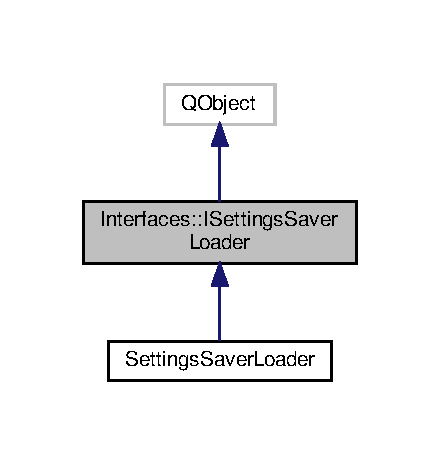
\includegraphics[width=211pt]{class_interfaces_1_1_i_settings_saver_loader__inherit__graph}
\end{center}
\end{figure}


Collaboration diagram for Interfaces\+:\+:I\+Settings\+Saver\+Loader\+:\nopagebreak
\begin{figure}[H]
\begin{center}
\leavevmode
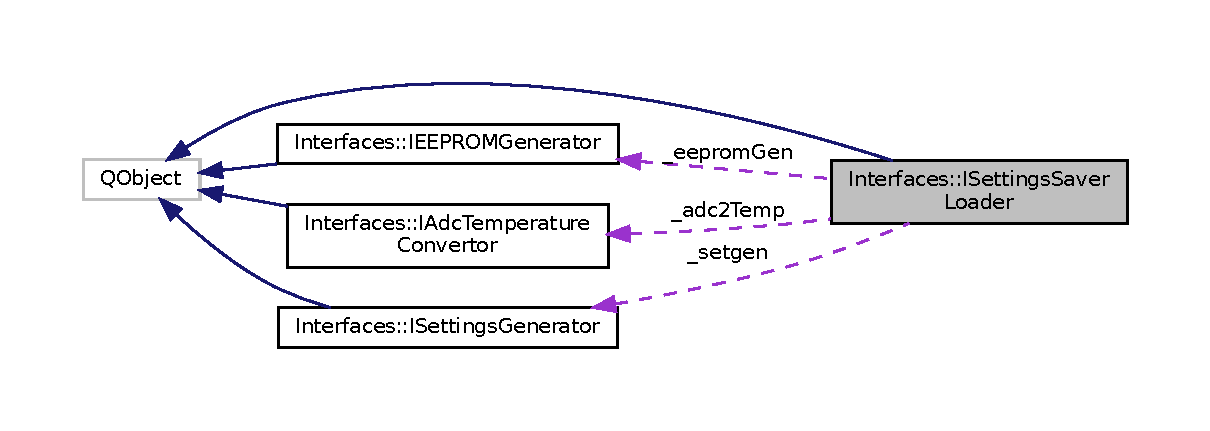
\includegraphics[width=350pt]{class_interfaces_1_1_i_settings_saver_loader__coll__graph}
\end{center}
\end{figure}
\subsection*{Public Member Functions}
\begin{DoxyCompactItemize}
\item 
virtual void \hyperlink{class_interfaces_1_1_i_settings_saver_loader_a67e729cc53f53b6bdeb534dc62000531}{Create} (Q\+String path, Q\+String adc2\+Temp\+Path)=0
\begin{DoxyCompactList}\small\item\em Creates settings file at path and embeds A\+D\+C-\/$>$Temperature settings from adc2\+Temp\+Path into it. \end{DoxyCompactList}\item 
virtual bool \hyperlink{class_interfaces_1_1_i_settings_saver_loader_a4d8bdb2c5a27b5b0aa5ee4e55483f0de}{Load} (Q\+String path)=0
\begin{DoxyCompactList}\small\item\em Loads settings from given file. \end{DoxyCompactList}\item 
\mbox{\Hypertarget{class_interfaces_1_1_i_settings_saver_loader_a5434144e59300dd6ed380f9600870cfa}\label{class_interfaces_1_1_i_settings_saver_loader_a5434144e59300dd6ed380f9600870cfa}} 
virtual void \hyperlink{class_interfaces_1_1_i_settings_saver_loader_a5434144e59300dd6ed380f9600870cfa}{Save} ()=0
\begin{DoxyCompactList}\small\item\em Saves settings to current file or throws exception if current file is not set. \end{DoxyCompactList}\item 
virtual void \hyperlink{class_interfaces_1_1_i_settings_saver_loader_a2d6a6dd6e5b6fe15e8b78af2e75725fc}{Save\+As} (Q\+String path)=0
\begin{DoxyCompactList}\small\item\em Saves settings to given file, then sets this file as current. \end{DoxyCompactList}\item 
virtual Q\+String \hyperlink{class_interfaces_1_1_i_settings_saver_loader_a7224c9ffc2d9c6a3b98fb20246e97cc3}{Get\+File\+Path} ()=0
\begin{DoxyCompactList}\small\item\em Get\+File\+Path Returns current file full path. If null then file wasn\textquotesingle{}t loaded/created at all. \end{DoxyCompactList}\item 
\mbox{\Hypertarget{class_interfaces_1_1_i_settings_saver_loader_aba09cbe4cc05e6cef67c41789bdccd23}\label{class_interfaces_1_1_i_settings_saver_loader_aba09cbe4cc05e6cef67c41789bdccd23}} 
virtual void \hyperlink{class_interfaces_1_1_i_settings_saver_loader_aba09cbe4cc05e6cef67c41789bdccd23}{Mark\+As\+Modified} ()=0
\begin{DoxyCompactList}\small\item\em Makrs current file is modified. If no file loaded does nothing. \end{DoxyCompactList}\item 
virtual bool \hyperlink{class_interfaces_1_1_i_settings_saver_loader_a4c3f69d0bc7c355030c8d371367108d3}{Is\+Modified} ()=0
\begin{DoxyCompactList}\small\item\em Is\+Modified True if file was modified and haven\textquotesingle{}t saved till now. \end{DoxyCompactList}\item 
virtual \hyperlink{class_interfaces_1_1_i_adc_temperature_convertor}{Interfaces\+::\+I\+Adc\+Temperature\+Convertor} $\ast$ \hyperlink{class_interfaces_1_1_i_settings_saver_loader_a44d68d2bc7de1717bc41ee264db13ac5}{Get\+A\+D\+C2\+Temp\+Convertor\+Ptr} ()=0
\begin{DoxyCompactList}\small\item\em Returns pointer to A\+D\+C-\/$>$Temperature convertor instance. \end{DoxyCompactList}\item 
virtual \hyperlink{class_interfaces_1_1_i_settings_generator}{Interfaces\+::\+I\+Settings\+Generator} $\ast$ \hyperlink{class_interfaces_1_1_i_settings_saver_loader_a73c8012dc63ca02d65a013ca901840ba}{Get\+Settings\+Generator\+Ptr} ()=0
\begin{DoxyCompactList}\small\item\em Returns pointer to settings generator. \end{DoxyCompactList}\item 
virtual void \hyperlink{class_interfaces_1_1_i_settings_saver_loader_a4f855492363276d81031d931a72a49a3}{Export\+To\+E\+E\+P\+R\+OM} (Q\+String path)=0
\begin{DoxyCompactList}\small\item\em Export current settings to E\+E\+P\+R\+OM file at given path. \end{DoxyCompactList}\end{DoxyCompactItemize}
\subsection*{Protected Attributes}
\begin{DoxyCompactItemize}
\item 
\mbox{\Hypertarget{class_interfaces_1_1_i_settings_saver_loader_accc3becffc7bb3688db96f3f34a68b80}\label{class_interfaces_1_1_i_settings_saver_loader_accc3becffc7bb3688db96f3f34a68b80}} 
\hyperlink{class_interfaces_1_1_i_adc_temperature_convertor}{Interfaces\+::\+I\+Adc\+Temperature\+Convertor} $\ast$ \hyperlink{class_interfaces_1_1_i_settings_saver_loader_accc3becffc7bb3688db96f3f34a68b80}{\+\_\+adc2\+Temp} = nullptr
\begin{DoxyCompactList}\small\item\em A\+DC to temperature convertor. \end{DoxyCompactList}\item 
\mbox{\Hypertarget{class_interfaces_1_1_i_settings_saver_loader_a7b2968ed33e6f5e2cc3b863649aa7f17}\label{class_interfaces_1_1_i_settings_saver_loader_a7b2968ed33e6f5e2cc3b863649aa7f17}} 
\hyperlink{class_interfaces_1_1_i_settings_generator}{Interfaces\+::\+I\+Settings\+Generator} $\ast$ \hyperlink{class_interfaces_1_1_i_settings_saver_loader_a7b2968ed33e6f5e2cc3b863649aa7f17}{\+\_\+setgen} = nullptr
\begin{DoxyCompactList}\small\item\em Settings generator. \end{DoxyCompactList}\item 
\mbox{\Hypertarget{class_interfaces_1_1_i_settings_saver_loader_a14446fa4caf99dcbfd748eaaa4ef3596}\label{class_interfaces_1_1_i_settings_saver_loader_a14446fa4caf99dcbfd748eaaa4ef3596}} 
\hyperlink{class_interfaces_1_1_i_e_e_p_r_o_m_generator}{Interfaces\+::\+I\+E\+E\+P\+R\+O\+M\+Generator} $\ast$ \hyperlink{class_interfaces_1_1_i_settings_saver_loader_a14446fa4caf99dcbfd748eaaa4ef3596}{\+\_\+eeprom\+Gen} = nullptr
\begin{DoxyCompactList}\small\item\em E\+E\+P\+R\+OM contents generator. \end{DoxyCompactList}\end{DoxyCompactItemize}


\subsection{Detailed Description}
Interface to save and load controller settings into X\+ML. 

Definition at line 34 of file I\+Settings\+Saver\+Loader.\+hpp.



\subsection{Member Function Documentation}
\mbox{\Hypertarget{class_interfaces_1_1_i_settings_saver_loader_a67e729cc53f53b6bdeb534dc62000531}\label{class_interfaces_1_1_i_settings_saver_loader_a67e729cc53f53b6bdeb534dc62000531}} 
\index{Interfaces\+::\+I\+Settings\+Saver\+Loader@{Interfaces\+::\+I\+Settings\+Saver\+Loader}!Create@{Create}}
\index{Create@{Create}!Interfaces\+::\+I\+Settings\+Saver\+Loader@{Interfaces\+::\+I\+Settings\+Saver\+Loader}}
\subsubsection{\texorpdfstring{Create()}{Create()}}
{\footnotesize\ttfamily virtual void Interfaces\+::\+I\+Settings\+Saver\+Loader\+::\+Create (\begin{DoxyParamCaption}\item[{Q\+String}]{path,  }\item[{Q\+String}]{adc2\+Temp\+Path }\end{DoxyParamCaption})\hspace{0.3cm}{\ttfamily [pure virtual]}}



Creates settings file at path and embeds A\+D\+C-\/$>$Temperature settings from adc2\+Temp\+Path into it. 


\begin{DoxyParams}{Parameters}
{\em path} & Path where created file will be stored (actual write occurs on \char`\"{}\+Save\char`\"{} call). \\
\hline
{\em adc2\+Temp\+Path} & path to file with A\+D\+C-\/$>$Temperature settings. \\
\hline
\end{DoxyParams}


Implemented in \hyperlink{class_settings_saver_loader_a23524241e3edea7f26b72807c0090bdc}{Settings\+Saver\+Loader}.

\mbox{\Hypertarget{class_interfaces_1_1_i_settings_saver_loader_a4f855492363276d81031d931a72a49a3}\label{class_interfaces_1_1_i_settings_saver_loader_a4f855492363276d81031d931a72a49a3}} 
\index{Interfaces\+::\+I\+Settings\+Saver\+Loader@{Interfaces\+::\+I\+Settings\+Saver\+Loader}!Export\+To\+E\+E\+P\+R\+OM@{Export\+To\+E\+E\+P\+R\+OM}}
\index{Export\+To\+E\+E\+P\+R\+OM@{Export\+To\+E\+E\+P\+R\+OM}!Interfaces\+::\+I\+Settings\+Saver\+Loader@{Interfaces\+::\+I\+Settings\+Saver\+Loader}}
\subsubsection{\texorpdfstring{Export\+To\+E\+E\+P\+R\+O\+M()}{ExportToEEPROM()}}
{\footnotesize\ttfamily virtual void Interfaces\+::\+I\+Settings\+Saver\+Loader\+::\+Export\+To\+E\+E\+P\+R\+OM (\begin{DoxyParamCaption}\item[{Q\+String}]{path }\end{DoxyParamCaption})\hspace{0.3cm}{\ttfamily [pure virtual]}}



Export current settings to E\+E\+P\+R\+OM file at given path. 


\begin{DoxyParams}{Parameters}
{\em path} & File, where E\+E\+P\+R\+OM contents will be saved. \\
\hline
\end{DoxyParams}


Implemented in \hyperlink{class_settings_saver_loader_a2a3e3c7f6f1f521b9423db4d63ddae74}{Settings\+Saver\+Loader}.

\mbox{\Hypertarget{class_interfaces_1_1_i_settings_saver_loader_a44d68d2bc7de1717bc41ee264db13ac5}\label{class_interfaces_1_1_i_settings_saver_loader_a44d68d2bc7de1717bc41ee264db13ac5}} 
\index{Interfaces\+::\+I\+Settings\+Saver\+Loader@{Interfaces\+::\+I\+Settings\+Saver\+Loader}!Get\+A\+D\+C2\+Temp\+Convertor\+Ptr@{Get\+A\+D\+C2\+Temp\+Convertor\+Ptr}}
\index{Get\+A\+D\+C2\+Temp\+Convertor\+Ptr@{Get\+A\+D\+C2\+Temp\+Convertor\+Ptr}!Interfaces\+::\+I\+Settings\+Saver\+Loader@{Interfaces\+::\+I\+Settings\+Saver\+Loader}}
\subsubsection{\texorpdfstring{Get\+A\+D\+C2\+Temp\+Convertor\+Ptr()}{GetADC2TempConvertorPtr()}}
{\footnotesize\ttfamily virtual \hyperlink{class_interfaces_1_1_i_adc_temperature_convertor}{Interfaces\+::\+I\+Adc\+Temperature\+Convertor}$\ast$ Interfaces\+::\+I\+Settings\+Saver\+Loader\+::\+Get\+A\+D\+C2\+Temp\+Convertor\+Ptr (\begin{DoxyParamCaption}{ }\end{DoxyParamCaption})\hspace{0.3cm}{\ttfamily [pure virtual]}}



Returns pointer to A\+D\+C-\/$>$Temperature convertor instance. 

\begin{DoxyReturn}{Returns}
Pointer to A\+D\+C-\/$>$Temperature convertor. 
\end{DoxyReturn}


Implemented in \hyperlink{class_settings_saver_loader_aa1265b1e9431bf3b611e5b45b4782700}{Settings\+Saver\+Loader}.

\mbox{\Hypertarget{class_interfaces_1_1_i_settings_saver_loader_a7224c9ffc2d9c6a3b98fb20246e97cc3}\label{class_interfaces_1_1_i_settings_saver_loader_a7224c9ffc2d9c6a3b98fb20246e97cc3}} 
\index{Interfaces\+::\+I\+Settings\+Saver\+Loader@{Interfaces\+::\+I\+Settings\+Saver\+Loader}!Get\+File\+Path@{Get\+File\+Path}}
\index{Get\+File\+Path@{Get\+File\+Path}!Interfaces\+::\+I\+Settings\+Saver\+Loader@{Interfaces\+::\+I\+Settings\+Saver\+Loader}}
\subsubsection{\texorpdfstring{Get\+File\+Path()}{GetFilePath()}}
{\footnotesize\ttfamily virtual Q\+String Interfaces\+::\+I\+Settings\+Saver\+Loader\+::\+Get\+File\+Path (\begin{DoxyParamCaption}{ }\end{DoxyParamCaption})\hspace{0.3cm}{\ttfamily [pure virtual]}}



Get\+File\+Path Returns current file full path. If null then file wasn\textquotesingle{}t loaded/created at all. 

\begin{DoxyReturn}{Returns}
Current file path. 
\end{DoxyReturn}


Implemented in \hyperlink{class_settings_saver_loader_a006a6350a00ffc18ec544616e504ccf7}{Settings\+Saver\+Loader}.

\mbox{\Hypertarget{class_interfaces_1_1_i_settings_saver_loader_a73c8012dc63ca02d65a013ca901840ba}\label{class_interfaces_1_1_i_settings_saver_loader_a73c8012dc63ca02d65a013ca901840ba}} 
\index{Interfaces\+::\+I\+Settings\+Saver\+Loader@{Interfaces\+::\+I\+Settings\+Saver\+Loader}!Get\+Settings\+Generator\+Ptr@{Get\+Settings\+Generator\+Ptr}}
\index{Get\+Settings\+Generator\+Ptr@{Get\+Settings\+Generator\+Ptr}!Interfaces\+::\+I\+Settings\+Saver\+Loader@{Interfaces\+::\+I\+Settings\+Saver\+Loader}}
\subsubsection{\texorpdfstring{Get\+Settings\+Generator\+Ptr()}{GetSettingsGeneratorPtr()}}
{\footnotesize\ttfamily virtual \hyperlink{class_interfaces_1_1_i_settings_generator}{Interfaces\+::\+I\+Settings\+Generator}$\ast$ Interfaces\+::\+I\+Settings\+Saver\+Loader\+::\+Get\+Settings\+Generator\+Ptr (\begin{DoxyParamCaption}{ }\end{DoxyParamCaption})\hspace{0.3cm}{\ttfamily [pure virtual]}}



Returns pointer to settings generator. 

\begin{DoxyReturn}{Returns}
Pointer to settings generator. 
\end{DoxyReturn}


Implemented in \hyperlink{class_settings_saver_loader_aa6b0a9b4f42335b03341a13f8bfff845}{Settings\+Saver\+Loader}.

\mbox{\Hypertarget{class_interfaces_1_1_i_settings_saver_loader_a4c3f69d0bc7c355030c8d371367108d3}\label{class_interfaces_1_1_i_settings_saver_loader_a4c3f69d0bc7c355030c8d371367108d3}} 
\index{Interfaces\+::\+I\+Settings\+Saver\+Loader@{Interfaces\+::\+I\+Settings\+Saver\+Loader}!Is\+Modified@{Is\+Modified}}
\index{Is\+Modified@{Is\+Modified}!Interfaces\+::\+I\+Settings\+Saver\+Loader@{Interfaces\+::\+I\+Settings\+Saver\+Loader}}
\subsubsection{\texorpdfstring{Is\+Modified()}{IsModified()}}
{\footnotesize\ttfamily virtual bool Interfaces\+::\+I\+Settings\+Saver\+Loader\+::\+Is\+Modified (\begin{DoxyParamCaption}{ }\end{DoxyParamCaption})\hspace{0.3cm}{\ttfamily [pure virtual]}}



Is\+Modified True if file was modified and haven\textquotesingle{}t saved till now. 

\begin{DoxyReturn}{Returns}
True if file modified. 
\end{DoxyReturn}


Implemented in \hyperlink{class_settings_saver_loader_a35574bdfc340a148245ea8017c59f2eb}{Settings\+Saver\+Loader}.

\mbox{\Hypertarget{class_interfaces_1_1_i_settings_saver_loader_a4d8bdb2c5a27b5b0aa5ee4e55483f0de}\label{class_interfaces_1_1_i_settings_saver_loader_a4d8bdb2c5a27b5b0aa5ee4e55483f0de}} 
\index{Interfaces\+::\+I\+Settings\+Saver\+Loader@{Interfaces\+::\+I\+Settings\+Saver\+Loader}!Load@{Load}}
\index{Load@{Load}!Interfaces\+::\+I\+Settings\+Saver\+Loader@{Interfaces\+::\+I\+Settings\+Saver\+Loader}}
\subsubsection{\texorpdfstring{Load()}{Load()}}
{\footnotesize\ttfamily virtual bool Interfaces\+::\+I\+Settings\+Saver\+Loader\+::\+Load (\begin{DoxyParamCaption}\item[{Q\+String}]{path }\end{DoxyParamCaption})\hspace{0.3cm}{\ttfamily [pure virtual]}}



Loads settings from given file. 


\begin{DoxyParams}{Parameters}
{\em path} & File to load from. \\
\hline
\end{DoxyParams}
\begin{DoxyReturn}{Returns}
True if load successful. 
\end{DoxyReturn}


Implemented in \hyperlink{class_settings_saver_loader_aaf225d7d568ce33f6350d886bb40312a}{Settings\+Saver\+Loader}.

\mbox{\Hypertarget{class_interfaces_1_1_i_settings_saver_loader_a2d6a6dd6e5b6fe15e8b78af2e75725fc}\label{class_interfaces_1_1_i_settings_saver_loader_a2d6a6dd6e5b6fe15e8b78af2e75725fc}} 
\index{Interfaces\+::\+I\+Settings\+Saver\+Loader@{Interfaces\+::\+I\+Settings\+Saver\+Loader}!Save\+As@{Save\+As}}
\index{Save\+As@{Save\+As}!Interfaces\+::\+I\+Settings\+Saver\+Loader@{Interfaces\+::\+I\+Settings\+Saver\+Loader}}
\subsubsection{\texorpdfstring{Save\+As()}{SaveAs()}}
{\footnotesize\ttfamily virtual void Interfaces\+::\+I\+Settings\+Saver\+Loader\+::\+Save\+As (\begin{DoxyParamCaption}\item[{Q\+String}]{path }\end{DoxyParamCaption})\hspace{0.3cm}{\ttfamily [pure virtual]}}



Saves settings to given file, then sets this file as current. 


\begin{DoxyParams}{Parameters}
{\em path} & Path to save. \\
\hline
\end{DoxyParams}


Implemented in \hyperlink{class_settings_saver_loader_a67b93496f8b0a0a779d783e967d93572}{Settings\+Saver\+Loader}.



The documentation for this class was generated from the following file\+:\begin{DoxyCompactItemize}
\item 
Interfaces/I\+Settings\+Saver\+Loader.\+hpp\end{DoxyCompactItemize}

\hypertarget{class_interfaces_1_1_i_settings_step}{}\section{Interfaces\+:\+:I\+Settings\+Step Class Reference}
\label{class_interfaces_1_1_i_settings_step}\index{Interfaces\+::\+I\+Settings\+Step@{Interfaces\+::\+I\+Settings\+Step}}


Interface with one settings step (i.\+e. with temperature and R\+PM percent increments)  




{\ttfamily \#include $<$I\+Settings\+Step.\+hpp$>$}



Inheritance diagram for Interfaces\+:\+:I\+Settings\+Step\+:\nopagebreak
\begin{figure}[H]
\begin{center}
\leavevmode
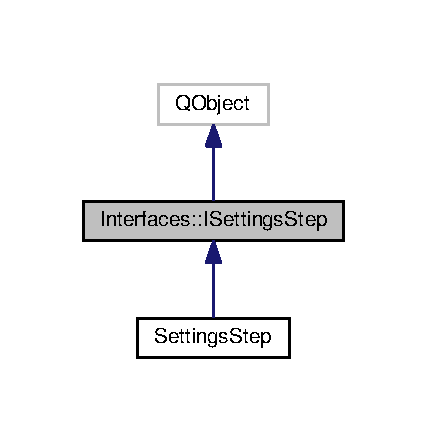
\includegraphics[width=205pt]{class_interfaces_1_1_i_settings_step__inherit__graph}
\end{center}
\end{figure}


Collaboration diagram for Interfaces\+:\+:I\+Settings\+Step\+:\nopagebreak
\begin{figure}[H]
\begin{center}
\leavevmode
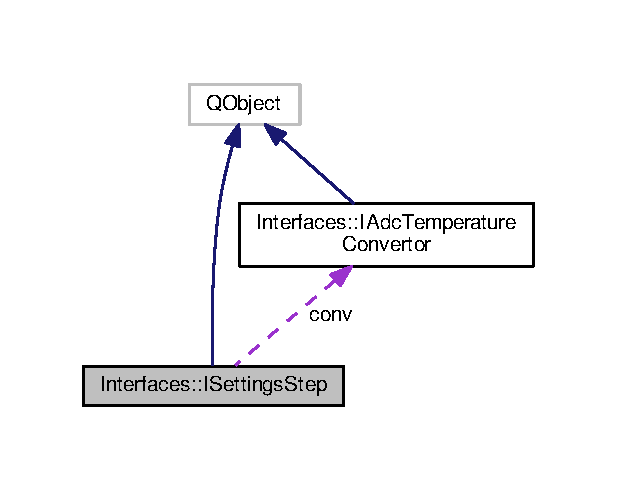
\includegraphics[width=296pt]{class_interfaces_1_1_i_settings_step__coll__graph}
\end{center}
\end{figure}
\subsection*{Public Member Functions}
\begin{DoxyCompactItemize}
\item 
virtual void \hyperlink{class_interfaces_1_1_i_settings_step_a04e46c3ebe1f28e0ad0bce23fb863f66}{Calculate\+Primary\+Values} (uint previous\+\_\+adc, uint previous\+\_\+rpm)=0
\begin{DoxyCompactList}\small\item\em Calculates primary values (i.\+e. current A\+DC level and current R\+PM) basing on previus step values. If resulting A\+DC / R\+PM levels will be greater than A\+D\+C\+\_\+\+M\+A\+X\+\_\+\+V\+A\+L\+UE / M\+A\+X\+\_\+\+R\+PM respectively, then levels will be set to A\+D\+C\+\_\+\+M\+A\+X\+\_\+\+V\+A\+L\+UE / M\+A\+X\+\_\+\+R\+PM. \end{DoxyCompactList}\item 
virtual Q\+String \hyperlink{class_interfaces_1_1_i_settings_step_a7575d43b7d178d700e161ec48e2c766f}{Get\+Current\+R\+P\+M\+Percents\+String} ()=0
\begin{DoxyCompactList}\small\item\em Returns \char`\"{}\+Off\char`\"{} if \+\_\+\+Current\+R\+PM == 0, and string representation of \hyperlink{class_interfaces_1_1_i_settings_step_abbbb49e91352212c6201a85f1a22253f}{Get\+Current\+R\+P\+M\+Percents()} otherwise. \end{DoxyCompactList}\item 
virtual void \hyperlink{class_interfaces_1_1_i_settings_step_a83f00b8b66f6566721065e34e41508c6}{Set\+A\+D\+C\+Delta} (uint delta, bool skip\+Limits\+Check=false)=0
\begin{DoxyCompactList}\small\item\em Call it to set A\+DC delta value. If delta more than M\+A\+X\+\_\+\+A\+D\+C\+\_\+\+D\+E\+L\+TA (defined in descendant) set it to M\+A\+X\+\_\+\+A\+D\+C\+\_\+\+D\+E\+L\+TA, if it less then M\+I\+N\+\_\+\+A\+D\+C\+\_\+\+D\+E\+L\+TA -\/ set it to M\+I\+N\+\_\+\+A\+D\+C\+\_\+\+D\+E\+L\+TA. \end{DoxyCompactList}\item 
virtual uint \hyperlink{class_interfaces_1_1_i_settings_step_ab77c6eaa45707ec4932a8f432b13ad78}{Get\+A\+D\+C\+Delta} ()=0
\begin{DoxyCompactList}\small\item\em Returns current A\+DC delta. \end{DoxyCompactList}\item 
virtual double \hyperlink{class_interfaces_1_1_i_settings_step_a7dd93517fbd9bc10a54b3b35a2f8bd78}{Get\+Temp\+Delta} ()=0
\begin{DoxyCompactList}\small\item\em As \hyperlink{class_interfaces_1_1_i_settings_step_ab77c6eaa45707ec4932a8f432b13ad78}{Get\+A\+D\+C\+Delta()}, but returns current A\+DC delta, converted to Celsius. \end{DoxyCompactList}\item 
virtual void \hyperlink{class_interfaces_1_1_i_settings_step_a62997701dc6ad91ec0a9d699ef99463e}{Set\+R\+P\+M\+Delta} (uint delta, bool skip\+Limits\+Check=false)=0
\begin{DoxyCompactList}\small\item\em Like \hyperlink{class_interfaces_1_1_i_settings_step_a83f00b8b66f6566721065e34e41508c6}{Set\+A\+D\+C\+Delta()}, but for R\+PM delta. Making check for M\+A\+X\+\_\+\+R\+P\+M\+\_\+\+D\+E\+L\+TA, if delta is greater then it, delta will be M\+A\+X\+\_\+\+R\+P\+M\+\_\+\+D\+E\+L\+TA. \end{DoxyCompactList}\item 
virtual uint \hyperlink{class_interfaces_1_1_i_settings_step_ace758dafae2a6bcbb0b1a3a64c802e3c}{Get\+R\+P\+M\+Delta} ()=0
\begin{DoxyCompactList}\small\item\em As \hyperlink{class_interfaces_1_1_i_settings_step_ab77c6eaa45707ec4932a8f432b13ad78}{Get\+A\+D\+C\+Delta()}, but for R\+PM delta. \end{DoxyCompactList}\item 
virtual double \hyperlink{class_interfaces_1_1_i_settings_step_a9db8c7569c5dc35b8541dc6e4d202df1}{Get\+R\+P\+M\+Delta\+Percents} ()=0
\begin{DoxyCompactList}\small\item\em As \hyperlink{class_interfaces_1_1_i_settings_step_ace758dafae2a6bcbb0b1a3a64c802e3c}{Get\+R\+P\+M\+Delta()}, but in percents. \end{DoxyCompactList}\item 
virtual uint \hyperlink{class_interfaces_1_1_i_settings_step_a54d5ce3350791e080bcb75d472376abf}{Get\+Current\+A\+DC} ()=0
\begin{DoxyCompactList}\small\item\em Returns A\+DC level for this step. \end{DoxyCompactList}\item 
virtual uint \hyperlink{class_interfaces_1_1_i_settings_step_ac2b2370bf70fb09a9e1da4db922e8903}{Get\+Current\+R\+PM} ()=0
\begin{DoxyCompactList}\small\item\em Get current R\+PM setting (see \hyperlink{_i_settings_generator_8hpp_source}{Interfaces/\+I\+Settings\+Generator.\+hpp} for details) \end{DoxyCompactList}\item 
virtual double \hyperlink{class_interfaces_1_1_i_settings_step_a62644690b7b63d27e72eca277a32bfdd}{Get\+Current\+Temperature} ()=0
\begin{DoxyCompactList}\small\item\em As \hyperlink{class_interfaces_1_1_i_settings_step_a54d5ce3350791e080bcb75d472376abf}{Get\+Current\+A\+D\+C()}, but returns temperature in Celsius. \end{DoxyCompactList}\item 
virtual double \hyperlink{class_interfaces_1_1_i_settings_step_abbbb49e91352212c6201a85f1a22253f}{Get\+Current\+R\+P\+M\+Percents} ()=0
\begin{DoxyCompactList}\small\item\em As \hyperlink{class_interfaces_1_1_i_settings_step_ac2b2370bf70fb09a9e1da4db922e8903}{Get\+Current\+R\+P\+M()}, but returns value in percents. \end{DoxyCompactList}\end{DoxyCompactItemize}
\subsection*{Protected Attributes}
\begin{DoxyCompactItemize}
\item 
\mbox{\Hypertarget{class_interfaces_1_1_i_settings_step_a5db60ca3f2c1b4e7059910e2d86656b9}\label{class_interfaces_1_1_i_settings_step_a5db60ca3f2c1b4e7059910e2d86656b9}} 
\hyperlink{class_interfaces_1_1_i_adc_temperature_convertor}{Interfaces\+::\+I\+Adc\+Temperature\+Convertor} $\ast$ \hyperlink{class_interfaces_1_1_i_settings_step_a5db60ca3f2c1b4e7059910e2d86656b9}{conv} = 0
\begin{DoxyCompactList}\small\item\em A\+DC$<$-\/$>$Temperature convertor. \end{DoxyCompactList}\end{DoxyCompactItemize}


\subsection{Detailed Description}
Interface with one settings step (i.\+e. with temperature and R\+PM percent increments) 

Definition at line 33 of file I\+Settings\+Step.\+hpp.



\subsection{Member Function Documentation}
\mbox{\Hypertarget{class_interfaces_1_1_i_settings_step_a04e46c3ebe1f28e0ad0bce23fb863f66}\label{class_interfaces_1_1_i_settings_step_a04e46c3ebe1f28e0ad0bce23fb863f66}} 
\index{Interfaces\+::\+I\+Settings\+Step@{Interfaces\+::\+I\+Settings\+Step}!Calculate\+Primary\+Values@{Calculate\+Primary\+Values}}
\index{Calculate\+Primary\+Values@{Calculate\+Primary\+Values}!Interfaces\+::\+I\+Settings\+Step@{Interfaces\+::\+I\+Settings\+Step}}
\subsubsection{\texorpdfstring{Calculate\+Primary\+Values()}{CalculatePrimaryValues()}}
{\footnotesize\ttfamily virtual void Interfaces\+::\+I\+Settings\+Step\+::\+Calculate\+Primary\+Values (\begin{DoxyParamCaption}\item[{uint}]{previous\+\_\+adc,  }\item[{uint}]{previous\+\_\+rpm }\end{DoxyParamCaption})\hspace{0.3cm}{\ttfamily [pure virtual]}}



Calculates primary values (i.\+e. current A\+DC level and current R\+PM) basing on previus step values. If resulting A\+DC / R\+PM levels will be greater than A\+D\+C\+\_\+\+M\+A\+X\+\_\+\+V\+A\+L\+UE / M\+A\+X\+\_\+\+R\+PM respectively, then levels will be set to A\+D\+C\+\_\+\+M\+A\+X\+\_\+\+V\+A\+L\+UE / M\+A\+X\+\_\+\+R\+PM. 


\begin{DoxyParams}{Parameters}
{\em previous\+\_\+adc} & Previous step A\+DC value \\
\hline
{\em previous\+\_\+rpm} & Previous step R\+PM value \\
\hline
\end{DoxyParams}


Implemented in \hyperlink{class_settings_step_ac6f79a139ab25cc50ed105f64fc9652f}{Settings\+Step}.

\mbox{\Hypertarget{class_interfaces_1_1_i_settings_step_ab77c6eaa45707ec4932a8f432b13ad78}\label{class_interfaces_1_1_i_settings_step_ab77c6eaa45707ec4932a8f432b13ad78}} 
\index{Interfaces\+::\+I\+Settings\+Step@{Interfaces\+::\+I\+Settings\+Step}!Get\+A\+D\+C\+Delta@{Get\+A\+D\+C\+Delta}}
\index{Get\+A\+D\+C\+Delta@{Get\+A\+D\+C\+Delta}!Interfaces\+::\+I\+Settings\+Step@{Interfaces\+::\+I\+Settings\+Step}}
\subsubsection{\texorpdfstring{Get\+A\+D\+C\+Delta()}{GetADCDelta()}}
{\footnotesize\ttfamily virtual uint Interfaces\+::\+I\+Settings\+Step\+::\+Get\+A\+D\+C\+Delta (\begin{DoxyParamCaption}{ }\end{DoxyParamCaption})\hspace{0.3cm}{\ttfamily [pure virtual]}}



Returns current A\+DC delta. 

\begin{DoxyReturn}{Returns}
A\+DC delta for this step 
\end{DoxyReturn}


Implemented in \hyperlink{class_settings_step_aee30aaa97692d6b546e9dd002900f52e}{Settings\+Step}.

\mbox{\Hypertarget{class_interfaces_1_1_i_settings_step_a54d5ce3350791e080bcb75d472376abf}\label{class_interfaces_1_1_i_settings_step_a54d5ce3350791e080bcb75d472376abf}} 
\index{Interfaces\+::\+I\+Settings\+Step@{Interfaces\+::\+I\+Settings\+Step}!Get\+Current\+A\+DC@{Get\+Current\+A\+DC}}
\index{Get\+Current\+A\+DC@{Get\+Current\+A\+DC}!Interfaces\+::\+I\+Settings\+Step@{Interfaces\+::\+I\+Settings\+Step}}
\subsubsection{\texorpdfstring{Get\+Current\+A\+D\+C()}{GetCurrentADC()}}
{\footnotesize\ttfamily virtual uint Interfaces\+::\+I\+Settings\+Step\+::\+Get\+Current\+A\+DC (\begin{DoxyParamCaption}{ }\end{DoxyParamCaption})\hspace{0.3cm}{\ttfamily [pure virtual]}}



Returns A\+DC level for this step. 

\begin{DoxyReturn}{Returns}
A\+DC level for this step 
\end{DoxyReturn}


Implemented in \hyperlink{class_settings_step_a443f5643d9b547632c261c5f3a4288f1}{Settings\+Step}.

\mbox{\Hypertarget{class_interfaces_1_1_i_settings_step_ac2b2370bf70fb09a9e1da4db922e8903}\label{class_interfaces_1_1_i_settings_step_ac2b2370bf70fb09a9e1da4db922e8903}} 
\index{Interfaces\+::\+I\+Settings\+Step@{Interfaces\+::\+I\+Settings\+Step}!Get\+Current\+R\+PM@{Get\+Current\+R\+PM}}
\index{Get\+Current\+R\+PM@{Get\+Current\+R\+PM}!Interfaces\+::\+I\+Settings\+Step@{Interfaces\+::\+I\+Settings\+Step}}
\subsubsection{\texorpdfstring{Get\+Current\+R\+P\+M()}{GetCurrentRPM()}}
{\footnotesize\ttfamily virtual uint Interfaces\+::\+I\+Settings\+Step\+::\+Get\+Current\+R\+PM (\begin{DoxyParamCaption}{ }\end{DoxyParamCaption})\hspace{0.3cm}{\ttfamily [pure virtual]}}



Get current R\+PM setting (see \hyperlink{_i_settings_generator_8hpp_source}{Interfaces/\+I\+Settings\+Generator.\+hpp} for details) 

\begin{DoxyReturn}{Returns}
Current step R\+PM setting 
\end{DoxyReturn}


Implemented in \hyperlink{class_settings_step_aaba560b593af9bc96eeed3db01a469f4}{Settings\+Step}.

\mbox{\Hypertarget{class_interfaces_1_1_i_settings_step_abbbb49e91352212c6201a85f1a22253f}\label{class_interfaces_1_1_i_settings_step_abbbb49e91352212c6201a85f1a22253f}} 
\index{Interfaces\+::\+I\+Settings\+Step@{Interfaces\+::\+I\+Settings\+Step}!Get\+Current\+R\+P\+M\+Percents@{Get\+Current\+R\+P\+M\+Percents}}
\index{Get\+Current\+R\+P\+M\+Percents@{Get\+Current\+R\+P\+M\+Percents}!Interfaces\+::\+I\+Settings\+Step@{Interfaces\+::\+I\+Settings\+Step}}
\subsubsection{\texorpdfstring{Get\+Current\+R\+P\+M\+Percents()}{GetCurrentRPMPercents()}}
{\footnotesize\ttfamily virtual double Interfaces\+::\+I\+Settings\+Step\+::\+Get\+Current\+R\+P\+M\+Percents (\begin{DoxyParamCaption}{ }\end{DoxyParamCaption})\hspace{0.3cm}{\ttfamily [pure virtual]}}



As \hyperlink{class_interfaces_1_1_i_settings_step_ac2b2370bf70fb09a9e1da4db922e8903}{Get\+Current\+R\+P\+M()}, but returns value in percents. 

\begin{DoxyReturn}{Returns}
Current step R\+PM setting in percents 
\end{DoxyReturn}


Implemented in \hyperlink{class_settings_step_a35bea9115637a0c848e8f827f2353c11}{Settings\+Step}.

\mbox{\Hypertarget{class_interfaces_1_1_i_settings_step_a7575d43b7d178d700e161ec48e2c766f}\label{class_interfaces_1_1_i_settings_step_a7575d43b7d178d700e161ec48e2c766f}} 
\index{Interfaces\+::\+I\+Settings\+Step@{Interfaces\+::\+I\+Settings\+Step}!Get\+Current\+R\+P\+M\+Percents\+String@{Get\+Current\+R\+P\+M\+Percents\+String}}
\index{Get\+Current\+R\+P\+M\+Percents\+String@{Get\+Current\+R\+P\+M\+Percents\+String}!Interfaces\+::\+I\+Settings\+Step@{Interfaces\+::\+I\+Settings\+Step}}
\subsubsection{\texorpdfstring{Get\+Current\+R\+P\+M\+Percents\+String()}{GetCurrentRPMPercentsString()}}
{\footnotesize\ttfamily virtual Q\+String Interfaces\+::\+I\+Settings\+Step\+::\+Get\+Current\+R\+P\+M\+Percents\+String (\begin{DoxyParamCaption}{ }\end{DoxyParamCaption})\hspace{0.3cm}{\ttfamily [pure virtual]}}



Returns \char`\"{}\+Off\char`\"{} if \+\_\+\+Current\+R\+PM == 0, and string representation of \hyperlink{class_interfaces_1_1_i_settings_step_abbbb49e91352212c6201a85f1a22253f}{Get\+Current\+R\+P\+M\+Percents()} otherwise. 

\begin{DoxyReturn}{Returns}
\char`\"{}\+Off\char`\"{} or current R\+P\+Ms as string with percents 
\end{DoxyReturn}


Implemented in \hyperlink{class_settings_step_a21e452401e180d6e114561a8b05ab1ae}{Settings\+Step}.

\mbox{\Hypertarget{class_interfaces_1_1_i_settings_step_a62644690b7b63d27e72eca277a32bfdd}\label{class_interfaces_1_1_i_settings_step_a62644690b7b63d27e72eca277a32bfdd}} 
\index{Interfaces\+::\+I\+Settings\+Step@{Interfaces\+::\+I\+Settings\+Step}!Get\+Current\+Temperature@{Get\+Current\+Temperature}}
\index{Get\+Current\+Temperature@{Get\+Current\+Temperature}!Interfaces\+::\+I\+Settings\+Step@{Interfaces\+::\+I\+Settings\+Step}}
\subsubsection{\texorpdfstring{Get\+Current\+Temperature()}{GetCurrentTemperature()}}
{\footnotesize\ttfamily virtual double Interfaces\+::\+I\+Settings\+Step\+::\+Get\+Current\+Temperature (\begin{DoxyParamCaption}{ }\end{DoxyParamCaption})\hspace{0.3cm}{\ttfamily [pure virtual]}}



As \hyperlink{class_interfaces_1_1_i_settings_step_a54d5ce3350791e080bcb75d472376abf}{Get\+Current\+A\+D\+C()}, but returns temperature in Celsius. 

\begin{DoxyReturn}{Returns}
Current step temperature in Celsius 
\end{DoxyReturn}


Implemented in \hyperlink{class_settings_step_a78ec872aa61713e3df36e93f56804afe}{Settings\+Step}.

\mbox{\Hypertarget{class_interfaces_1_1_i_settings_step_ace758dafae2a6bcbb0b1a3a64c802e3c}\label{class_interfaces_1_1_i_settings_step_ace758dafae2a6bcbb0b1a3a64c802e3c}} 
\index{Interfaces\+::\+I\+Settings\+Step@{Interfaces\+::\+I\+Settings\+Step}!Get\+R\+P\+M\+Delta@{Get\+R\+P\+M\+Delta}}
\index{Get\+R\+P\+M\+Delta@{Get\+R\+P\+M\+Delta}!Interfaces\+::\+I\+Settings\+Step@{Interfaces\+::\+I\+Settings\+Step}}
\subsubsection{\texorpdfstring{Get\+R\+P\+M\+Delta()}{GetRPMDelta()}}
{\footnotesize\ttfamily virtual uint Interfaces\+::\+I\+Settings\+Step\+::\+Get\+R\+P\+M\+Delta (\begin{DoxyParamCaption}{ }\end{DoxyParamCaption})\hspace{0.3cm}{\ttfamily [pure virtual]}}



As \hyperlink{class_interfaces_1_1_i_settings_step_ab77c6eaa45707ec4932a8f432b13ad78}{Get\+A\+D\+C\+Delta()}, but for R\+PM delta. 

\begin{DoxyReturn}{Returns}
R\+PM delta for this step 
\end{DoxyReturn}


Implemented in \hyperlink{class_settings_step_a594ce71fb0626c79c3e4d4f988e484af}{Settings\+Step}.

\mbox{\Hypertarget{class_interfaces_1_1_i_settings_step_a9db8c7569c5dc35b8541dc6e4d202df1}\label{class_interfaces_1_1_i_settings_step_a9db8c7569c5dc35b8541dc6e4d202df1}} 
\index{Interfaces\+::\+I\+Settings\+Step@{Interfaces\+::\+I\+Settings\+Step}!Get\+R\+P\+M\+Delta\+Percents@{Get\+R\+P\+M\+Delta\+Percents}}
\index{Get\+R\+P\+M\+Delta\+Percents@{Get\+R\+P\+M\+Delta\+Percents}!Interfaces\+::\+I\+Settings\+Step@{Interfaces\+::\+I\+Settings\+Step}}
\subsubsection{\texorpdfstring{Get\+R\+P\+M\+Delta\+Percents()}{GetRPMDeltaPercents()}}
{\footnotesize\ttfamily virtual double Interfaces\+::\+I\+Settings\+Step\+::\+Get\+R\+P\+M\+Delta\+Percents (\begin{DoxyParamCaption}{ }\end{DoxyParamCaption})\hspace{0.3cm}{\ttfamily [pure virtual]}}



As \hyperlink{class_interfaces_1_1_i_settings_step_ace758dafae2a6bcbb0b1a3a64c802e3c}{Get\+R\+P\+M\+Delta()}, but in percents. 

\begin{DoxyReturn}{Returns}
R\+PM delta for this step in percents 
\end{DoxyReturn}


Implemented in \hyperlink{class_settings_step_ada359fe4bfdaf271e621ec2943c0644c}{Settings\+Step}.

\mbox{\Hypertarget{class_interfaces_1_1_i_settings_step_a7dd93517fbd9bc10a54b3b35a2f8bd78}\label{class_interfaces_1_1_i_settings_step_a7dd93517fbd9bc10a54b3b35a2f8bd78}} 
\index{Interfaces\+::\+I\+Settings\+Step@{Interfaces\+::\+I\+Settings\+Step}!Get\+Temp\+Delta@{Get\+Temp\+Delta}}
\index{Get\+Temp\+Delta@{Get\+Temp\+Delta}!Interfaces\+::\+I\+Settings\+Step@{Interfaces\+::\+I\+Settings\+Step}}
\subsubsection{\texorpdfstring{Get\+Temp\+Delta()}{GetTempDelta()}}
{\footnotesize\ttfamily virtual double Interfaces\+::\+I\+Settings\+Step\+::\+Get\+Temp\+Delta (\begin{DoxyParamCaption}{ }\end{DoxyParamCaption})\hspace{0.3cm}{\ttfamily [pure virtual]}}



As \hyperlink{class_interfaces_1_1_i_settings_step_ab77c6eaa45707ec4932a8f432b13ad78}{Get\+A\+D\+C\+Delta()}, but returns current A\+DC delta, converted to Celsius. 

\begin{DoxyReturn}{Returns}
Celsuis representation of A\+DC delta 
\end{DoxyReturn}


Implemented in \hyperlink{class_settings_step_a8162810e5ce2df99053ac5722acc0901}{Settings\+Step}.

\mbox{\Hypertarget{class_interfaces_1_1_i_settings_step_a83f00b8b66f6566721065e34e41508c6}\label{class_interfaces_1_1_i_settings_step_a83f00b8b66f6566721065e34e41508c6}} 
\index{Interfaces\+::\+I\+Settings\+Step@{Interfaces\+::\+I\+Settings\+Step}!Set\+A\+D\+C\+Delta@{Set\+A\+D\+C\+Delta}}
\index{Set\+A\+D\+C\+Delta@{Set\+A\+D\+C\+Delta}!Interfaces\+::\+I\+Settings\+Step@{Interfaces\+::\+I\+Settings\+Step}}
\subsubsection{\texorpdfstring{Set\+A\+D\+C\+Delta()}{SetADCDelta()}}
{\footnotesize\ttfamily virtual void Interfaces\+::\+I\+Settings\+Step\+::\+Set\+A\+D\+C\+Delta (\begin{DoxyParamCaption}\item[{uint}]{delta,  }\item[{bool}]{skip\+Limits\+Check = {\ttfamily false} }\end{DoxyParamCaption})\hspace{0.3cm}{\ttfamily [pure virtual]}}



Call it to set A\+DC delta value. If delta more than M\+A\+X\+\_\+\+A\+D\+C\+\_\+\+D\+E\+L\+TA (defined in descendant) set it to M\+A\+X\+\_\+\+A\+D\+C\+\_\+\+D\+E\+L\+TA, if it less then M\+I\+N\+\_\+\+A\+D\+C\+\_\+\+D\+E\+L\+TA -\/ set it to M\+I\+N\+\_\+\+A\+D\+C\+\_\+\+D\+E\+L\+TA. 


\begin{DoxyParams}{Parameters}
{\em delta} & This value added to A\+DC value when we are going to next step (see Firmware/main.\+h E\+E\+P\+R\+OM S\+T\+R\+U\+C\+T\+U\+RE section for description) \\
\hline
{\em skip\+Limits\+Check} & If set to true, then checks for M\+I\+N\+\_\+\+A\+D\+C\+\_\+\+D\+E\+L\+TA and M\+A\+X\+\_\+\+A\+D\+C\+\_\+\+D\+E\+L\+TA will be skipped. Us it only for setting base level, because values outside \mbox{[}M\+I\+N\+\_\+\+A\+D\+C\+\_\+\+D\+E\+L\+T\+A-\/\+M\+A\+X\+\_\+\+A\+D\+C\+\_\+\+D\+E\+L\+TA\mbox{]} can\textquotesingle{}t be programmed into M\+CU. \\
\hline
\end{DoxyParams}


Implemented in \hyperlink{class_settings_step_a8124c87ae0b1d9fb3b623144d0e492db}{Settings\+Step}.

\mbox{\Hypertarget{class_interfaces_1_1_i_settings_step_a62997701dc6ad91ec0a9d699ef99463e}\label{class_interfaces_1_1_i_settings_step_a62997701dc6ad91ec0a9d699ef99463e}} 
\index{Interfaces\+::\+I\+Settings\+Step@{Interfaces\+::\+I\+Settings\+Step}!Set\+R\+P\+M\+Delta@{Set\+R\+P\+M\+Delta}}
\index{Set\+R\+P\+M\+Delta@{Set\+R\+P\+M\+Delta}!Interfaces\+::\+I\+Settings\+Step@{Interfaces\+::\+I\+Settings\+Step}}
\subsubsection{\texorpdfstring{Set\+R\+P\+M\+Delta()}{SetRPMDelta()}}
{\footnotesize\ttfamily virtual void Interfaces\+::\+I\+Settings\+Step\+::\+Set\+R\+P\+M\+Delta (\begin{DoxyParamCaption}\item[{uint}]{delta,  }\item[{bool}]{skip\+Limits\+Check = {\ttfamily false} }\end{DoxyParamCaption})\hspace{0.3cm}{\ttfamily [pure virtual]}}



Like \hyperlink{class_interfaces_1_1_i_settings_step_a83f00b8b66f6566721065e34e41508c6}{Set\+A\+D\+C\+Delta()}, but for R\+PM delta. Making check for M\+A\+X\+\_\+\+R\+P\+M\+\_\+\+D\+E\+L\+TA, if delta is greater then it, delta will be M\+A\+X\+\_\+\+R\+P\+M\+\_\+\+D\+E\+L\+TA. 


\begin{DoxyParams}{Parameters}
{\em delta} & This value added to R\+PM raw value when we are going to next step (see Firmware/main.\+h E\+E\+P\+R\+OM S\+T\+R\+U\+C\+T\+U\+RE section for description) \\
\hline
\end{DoxyParams}


Implemented in \hyperlink{class_settings_step_a25ddaf1d4d77727b8f87b5f8588f2de1}{Settings\+Step}.



The documentation for this class was generated from the following file\+:\begin{DoxyCompactItemize}
\item 
Interfaces/I\+Settings\+Step.\+hpp\end{DoxyCompactItemize}

\hypertarget{class_main_window}{}\section{Main\+Window Class Reference}
\label{class_main_window}\index{Main\+Window@{Main\+Window}}


Inheritance diagram for Main\+Window\+:\nopagebreak
\begin{figure}[H]
\begin{center}
\leavevmode
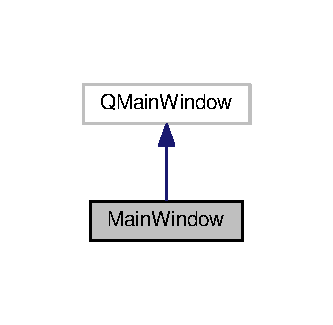
\includegraphics[width=160pt]{class_main_window__inherit__graph}
\end{center}
\end{figure}


Collaboration diagram for Main\+Window\+:\nopagebreak
\begin{figure}[H]
\begin{center}
\leavevmode
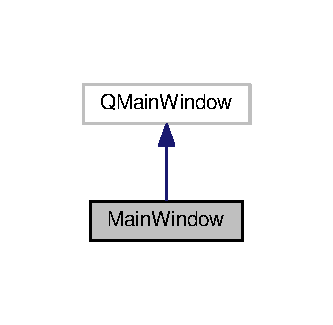
\includegraphics[width=160pt]{class_main_window__coll__graph}
\end{center}
\end{figure}
\subsection*{Public Slots}
\begin{DoxyCompactItemize}
\item 
\mbox{\Hypertarget{class_main_window_a95fb3a2c4f9240d386029d5ffebab1ac}\label{class_main_window_a95fb3a2c4f9240d386029d5ffebab1ac}} 
void \hyperlink{class_main_window_a95fb3a2c4f9240d386029d5ffebab1ac}{Mw\+Slot\+Exit} ()
\begin{DoxyCompactList}\small\item\em mn\+\_\+slot\+\_\+exit Called when user want to close application. \end{DoxyCompactList}\item 
\mbox{\Hypertarget{class_main_window_a2ef62a3653289364eace9bbf334d904b}\label{class_main_window_a2ef62a3653289364eace9bbf334d904b}} 
void \hyperlink{class_main_window_a2ef62a3653289364eace9bbf334d904b}{Mw\+Slot\+Create\+New\+A\+D\+C2\+Temp} ()
\begin{DoxyCompactList}\small\item\em Called when user wants to create a new A\+D\+C-\/$>$Temperature conversion settings. \end{DoxyCompactList}\item 
void \hyperlink{class_main_window_a0a690287dffb47b6477f2fb50c2a818e}{Mw\+Slot\+Base\+Temperature\+Changed} (double tempC)
\begin{DoxyCompactList}\small\item\em Called when user changes base temperature. \end{DoxyCompactList}\item 
void \hyperlink{class_main_window_aaf5b44955c0c93824ea89edd3cdc5730}{Mw\+Slot\+Base\+R\+P\+M\+Changed} (int R\+PM)
\begin{DoxyCompactList}\small\item\em Mw\+Slot\+Base\+R\+P\+M\+Changed Called when user changes base R\+PM level. \end{DoxyCompactList}\item 
void \hyperlink{class_main_window_acbdfd3592779f6946c4fecc33c79e9a4}{Mw\+Slot\+A\+D\+C\+Delta\+Changed\+Raw} (int new\+Delta)
\begin{DoxyCompactList}\small\item\em Called when A\+DC delta value of any spinbox is changed. It process change, determines what spinbox caused the change and then emits Mw\+A\+D\+C\+Delta\+Changed(uint Step\+Number, uint New\+Value) with step and new value. Connect all A\+DC delta spinboxes in steps table to it. \end{DoxyCompactList}\item 
void \hyperlink{class_main_window_a4480e7516f91b93c8abc3d42c1284124}{Mw\+Slot\+R\+P\+M\+Delta\+Changed\+Raw} (int new\+Delta)
\begin{DoxyCompactList}\small\item\em As \hyperlink{class_main_window_acbdfd3592779f6946c4fecc33c79e9a4}{Mw\+Slot\+A\+D\+C\+Delta\+Changed\+Raw()}, but for R\+PM delta. \end{DoxyCompactList}\item 
void \hyperlink{class_main_window_a5778840f76f8ce6edd63d84b57b801b1}{Mw\+Slot\+A\+D\+C\+Delta\+Changed} (uint Step\+Number, uint New\+Delta)
\begin{DoxyCompactList}\small\item\em Called when A\+DC delta value of any spinbox is chaned. \end{DoxyCompactList}\item 
void \hyperlink{class_main_window_a32b3a311b7151092db3ec0756d2c22d4}{Mw\+Slot\+R\+P\+M\+Delta\+Changed} (uint Step\+Number, uint New\+Delta)
\begin{DoxyCompactList}\small\item\em As \hyperlink{class_main_window_a5778840f76f8ce6edd63d84b57b801b1}{Mw\+Slot\+A\+D\+C\+Delta\+Changed()}, but for R\+PM Delta change. \end{DoxyCompactList}\item 
\mbox{\Hypertarget{class_main_window_a07c8e8c9d91588bdcc8e1eae01c4ffd7}\label{class_main_window_a07c8e8c9d91588bdcc8e1eae01c4ffd7}} 
void \hyperlink{class_main_window_a07c8e8c9d91588bdcc8e1eae01c4ffd7}{Mw\+Slot\+Update\+Steps\+Table} ()
\begin{DoxyCompactList}\small\item\em Updates UI steps table according to steps from settings generator. \end{DoxyCompactList}\item 
\mbox{\Hypertarget{class_main_window_ab2bca26ed91446c16caebf7a93ae1334}\label{class_main_window_ab2bca26ed91446c16caebf7a93ae1334}} 
void \hyperlink{class_main_window_ab2bca26ed91446c16caebf7a93ae1334}{Mw\+Slot\+Create\+File} ()
\begin{DoxyCompactList}\small\item\em Call this slot to create a new file. \end{DoxyCompactList}\item 
\mbox{\Hypertarget{class_main_window_a198ce62c26c57d653b0ac9f94eac87a4}\label{class_main_window_a198ce62c26c57d653b0ac9f94eac87a4}} 
void \hyperlink{class_main_window_a198ce62c26c57d653b0ac9f94eac87a4}{Mw\+Slot\+Save\+File} ()
\begin{DoxyCompactList}\small\item\em Call this slot to save file. \end{DoxyCompactList}\item 
\mbox{\Hypertarget{class_main_window_aaadd1a2cd4aec05d23e934a26ee3dbc6}\label{class_main_window_aaadd1a2cd4aec05d23e934a26ee3dbc6}} 
void \hyperlink{class_main_window_aaadd1a2cd4aec05d23e934a26ee3dbc6}{Mw\+Slot\+Save\+File\+As} ()
\begin{DoxyCompactList}\small\item\em Call it to save file under another name. \end{DoxyCompactList}\end{DoxyCompactItemize}
\subsection*{Signals}
\begin{DoxyCompactItemize}
\item 
\mbox{\Hypertarget{class_main_window_abc97afb888a70565123689a1444ab4b9}\label{class_main_window_abc97afb888a70565123689a1444ab4b9}} 
void \hyperlink{class_main_window_abc97afb888a70565123689a1444ab4b9}{Mw\+Signal\+Convertor\+Changed} ()
\begin{DoxyCompactList}\small\item\em Emit it when this-\/$>$tconv initialized with the new instance of A\+DC to Temperature convertor. \end{DoxyCompactList}\item 
void \hyperlink{class_main_window_a37ea64ccb9b5bcf9bb976602d42aadfa}{Mw\+Signal\+A\+D\+C\+Delta\+Changed} (uint Step\+Number, uint New\+Delta)
\begin{DoxyCompactList}\small\item\em Mw\+A\+D\+C\+Delta\+Changed Emitted when A\+DC delta changed for cell in steps table. \end{DoxyCompactList}\item 
void \hyperlink{class_main_window_a7b5fab96f0c2363958436141a3aae65b}{Mw\+Signal\+R\+P\+M\+Delta\+Changed} (uint Step\+Number, uint New\+Delta)
\begin{DoxyCompactList}\small\item\em As Mw\+A\+D\+C\+Delta\+Changed(), but for R\+PM delta. \end{DoxyCompactList}\item 
\mbox{\Hypertarget{class_main_window_abf2e8820a7173fb2231e7f835160d8a1}\label{class_main_window_abf2e8820a7173fb2231e7f835160d8a1}} 
void \hyperlink{class_main_window_abf2e8820a7173fb2231e7f835160d8a1}{Mw\+Signal\+Update\+Steps\+Table} ()
\begin{DoxyCompactList}\small\item\em Emit it when steps table (UI) needs to be re-\/read from settings generator. \end{DoxyCompactList}\end{DoxyCompactItemize}
\subsection*{Public Member Functions}
\begin{DoxyCompactItemize}
\item 
\mbox{\Hypertarget{class_main_window_a8b244be8b7b7db1b08de2a2acb9409db}\label{class_main_window_a8b244be8b7b7db1b08de2a2acb9409db}} 
{\bfseries Main\+Window} (Q\+Widget $\ast$parent=0)
\end{DoxyCompactItemize}
\subsection*{Protected Member Functions}
\begin{DoxyCompactItemize}
\item 
\mbox{\Hypertarget{class_main_window_af4ca5d0d3d18ddcb7d54b6596bbf4797}\label{class_main_window_af4ca5d0d3d18ddcb7d54b6596bbf4797}} 
void {\bfseries change\+Event} (Q\+Event $\ast$e)
\item 
\mbox{\Hypertarget{class_main_window_a8a5bf36f9544ed3ec3a9eea9b7154564}\label{class_main_window_a8a5bf36f9544ed3ec3a9eea9b7154564}} 
void {\bfseries close\+Event} (Q\+Close\+Event $\ast$e)
\end{DoxyCompactItemize}


\subsection{Detailed Description}


Definition at line 63 of file mainwindow.\+hpp.



\subsection{Member Function Documentation}
\mbox{\Hypertarget{class_main_window_a37ea64ccb9b5bcf9bb976602d42aadfa}\label{class_main_window_a37ea64ccb9b5bcf9bb976602d42aadfa}} 
\index{Main\+Window@{Main\+Window}!Mw\+Signal\+A\+D\+C\+Delta\+Changed@{Mw\+Signal\+A\+D\+C\+Delta\+Changed}}
\index{Mw\+Signal\+A\+D\+C\+Delta\+Changed@{Mw\+Signal\+A\+D\+C\+Delta\+Changed}!Main\+Window@{Main\+Window}}
\subsubsection{\texorpdfstring{Mw\+Signal\+A\+D\+C\+Delta\+Changed}{MwSignalADCDeltaChanged}}
{\footnotesize\ttfamily void Main\+Window\+::\+Mw\+Signal\+A\+D\+C\+Delta\+Changed (\begin{DoxyParamCaption}\item[{uint}]{Step\+Number,  }\item[{uint}]{New\+Delta }\end{DoxyParamCaption})\hspace{0.3cm}{\ttfamily [signal]}}



Mw\+A\+D\+C\+Delta\+Changed Emitted when A\+DC delta changed for cell in steps table. 


\begin{DoxyParams}{Parameters}
{\em Step\+Number} & -\/ Step number. \\
\hline
{\em New\+Value} & -\/ New A\+DC delta value. \\
\hline
\end{DoxyParams}
\mbox{\Hypertarget{class_main_window_a7b5fab96f0c2363958436141a3aae65b}\label{class_main_window_a7b5fab96f0c2363958436141a3aae65b}} 
\index{Main\+Window@{Main\+Window}!Mw\+Signal\+R\+P\+M\+Delta\+Changed@{Mw\+Signal\+R\+P\+M\+Delta\+Changed}}
\index{Mw\+Signal\+R\+P\+M\+Delta\+Changed@{Mw\+Signal\+R\+P\+M\+Delta\+Changed}!Main\+Window@{Main\+Window}}
\subsubsection{\texorpdfstring{Mw\+Signal\+R\+P\+M\+Delta\+Changed}{MwSignalRPMDeltaChanged}}
{\footnotesize\ttfamily void Main\+Window\+::\+Mw\+Signal\+R\+P\+M\+Delta\+Changed (\begin{DoxyParamCaption}\item[{uint}]{Step\+Number,  }\item[{uint}]{New\+Delta }\end{DoxyParamCaption})\hspace{0.3cm}{\ttfamily [signal]}}



As Mw\+A\+D\+C\+Delta\+Changed(), but for R\+PM delta. 


\begin{DoxyParams}{Parameters}
{\em Step\+Number} & See Mw\+A\+D\+C\+Delta\+Changed(). \\
\hline
{\em New\+Delta} & See Mw\+A\+D\+C\+Delta\+Changed(). \\
\hline
\end{DoxyParams}
\mbox{\Hypertarget{class_main_window_a5778840f76f8ce6edd63d84b57b801b1}\label{class_main_window_a5778840f76f8ce6edd63d84b57b801b1}} 
\index{Main\+Window@{Main\+Window}!Mw\+Slot\+A\+D\+C\+Delta\+Changed@{Mw\+Slot\+A\+D\+C\+Delta\+Changed}}
\index{Mw\+Slot\+A\+D\+C\+Delta\+Changed@{Mw\+Slot\+A\+D\+C\+Delta\+Changed}!Main\+Window@{Main\+Window}}
\subsubsection{\texorpdfstring{Mw\+Slot\+A\+D\+C\+Delta\+Changed}{MwSlotADCDeltaChanged}}
{\footnotesize\ttfamily void Main\+Window\+::\+Mw\+Slot\+A\+D\+C\+Delta\+Changed (\begin{DoxyParamCaption}\item[{uint}]{Step\+Number,  }\item[{uint}]{New\+Delta }\end{DoxyParamCaption})\hspace{0.3cm}{\ttfamily [slot]}}



Called when A\+DC delta value of any spinbox is chaned. 


\begin{DoxyParams}{Parameters}
{\em Step\+Number} & Step number, for what change occured. \\
\hline
{\em New\+Delta} & New A\+DC delta. \\
\hline
\end{DoxyParams}


Definition at line 293 of file mainwindow.\+cpp.

\mbox{\Hypertarget{class_main_window_acbdfd3592779f6946c4fecc33c79e9a4}\label{class_main_window_acbdfd3592779f6946c4fecc33c79e9a4}} 
\index{Main\+Window@{Main\+Window}!Mw\+Slot\+A\+D\+C\+Delta\+Changed\+Raw@{Mw\+Slot\+A\+D\+C\+Delta\+Changed\+Raw}}
\index{Mw\+Slot\+A\+D\+C\+Delta\+Changed\+Raw@{Mw\+Slot\+A\+D\+C\+Delta\+Changed\+Raw}!Main\+Window@{Main\+Window}}
\subsubsection{\texorpdfstring{Mw\+Slot\+A\+D\+C\+Delta\+Changed\+Raw}{MwSlotADCDeltaChangedRaw}}
{\footnotesize\ttfamily void Main\+Window\+::\+Mw\+Slot\+A\+D\+C\+Delta\+Changed\+Raw (\begin{DoxyParamCaption}\item[{int}]{new\+Delta }\end{DoxyParamCaption})\hspace{0.3cm}{\ttfamily [slot]}}



Called when A\+DC delta value of any spinbox is changed. It process change, determines what spinbox caused the change and then emits Mw\+A\+D\+C\+Delta\+Changed(uint Step\+Number, uint New\+Value) with step and new value. Connect all A\+DC delta spinboxes in steps table to it. 


\begin{DoxyParams}{Parameters}
{\em new\+Delta} & New delta value. \\
\hline
\end{DoxyParams}


Definition at line 267 of file mainwindow.\+cpp.

\mbox{\Hypertarget{class_main_window_aaf5b44955c0c93824ea89edd3cdc5730}\label{class_main_window_aaf5b44955c0c93824ea89edd3cdc5730}} 
\index{Main\+Window@{Main\+Window}!Mw\+Slot\+Base\+R\+P\+M\+Changed@{Mw\+Slot\+Base\+R\+P\+M\+Changed}}
\index{Mw\+Slot\+Base\+R\+P\+M\+Changed@{Mw\+Slot\+Base\+R\+P\+M\+Changed}!Main\+Window@{Main\+Window}}
\subsubsection{\texorpdfstring{Mw\+Slot\+Base\+R\+P\+M\+Changed}{MwSlotBaseRPMChanged}}
{\footnotesize\ttfamily void Main\+Window\+::\+Mw\+Slot\+Base\+R\+P\+M\+Changed (\begin{DoxyParamCaption}\item[{int}]{R\+PM }\end{DoxyParamCaption})\hspace{0.3cm}{\ttfamily [slot]}}



Mw\+Slot\+Base\+R\+P\+M\+Changed Called when user changes base R\+PM level. 


\begin{DoxyParams}{Parameters}
{\em R\+PM} & -\/ new R\+PM value \\
\hline
\end{DoxyParams}


Definition at line 199 of file mainwindow.\+cpp.

\mbox{\Hypertarget{class_main_window_a0a690287dffb47b6477f2fb50c2a818e}\label{class_main_window_a0a690287dffb47b6477f2fb50c2a818e}} 
\index{Main\+Window@{Main\+Window}!Mw\+Slot\+Base\+Temperature\+Changed@{Mw\+Slot\+Base\+Temperature\+Changed}}
\index{Mw\+Slot\+Base\+Temperature\+Changed@{Mw\+Slot\+Base\+Temperature\+Changed}!Main\+Window@{Main\+Window}}
\subsubsection{\texorpdfstring{Mw\+Slot\+Base\+Temperature\+Changed}{MwSlotBaseTemperatureChanged}}
{\footnotesize\ttfamily void Main\+Window\+::\+Mw\+Slot\+Base\+Temperature\+Changed (\begin{DoxyParamCaption}\item[{double}]{tempC }\end{DoxyParamCaption})\hspace{0.3cm}{\ttfamily [slot]}}



Called when user changes base temperature. 


\begin{DoxyParams}{Parameters}
{\em temp} & -\/ new temperature in Celsius \\
\hline
\end{DoxyParams}


Definition at line 181 of file mainwindow.\+cpp.

\mbox{\Hypertarget{class_main_window_a32b3a311b7151092db3ec0756d2c22d4}\label{class_main_window_a32b3a311b7151092db3ec0756d2c22d4}} 
\index{Main\+Window@{Main\+Window}!Mw\+Slot\+R\+P\+M\+Delta\+Changed@{Mw\+Slot\+R\+P\+M\+Delta\+Changed}}
\index{Mw\+Slot\+R\+P\+M\+Delta\+Changed@{Mw\+Slot\+R\+P\+M\+Delta\+Changed}!Main\+Window@{Main\+Window}}
\subsubsection{\texorpdfstring{Mw\+Slot\+R\+P\+M\+Delta\+Changed}{MwSlotRPMDeltaChanged}}
{\footnotesize\ttfamily void Main\+Window\+::\+Mw\+Slot\+R\+P\+M\+Delta\+Changed (\begin{DoxyParamCaption}\item[{uint}]{Step\+Number,  }\item[{uint}]{New\+Delta }\end{DoxyParamCaption})\hspace{0.3cm}{\ttfamily [slot]}}



As \hyperlink{class_main_window_a5778840f76f8ce6edd63d84b57b801b1}{Mw\+Slot\+A\+D\+C\+Delta\+Changed()}, but for R\+PM Delta change. 


\begin{DoxyParams}{Parameters}
{\em Step\+Number} & See \hyperlink{class_main_window_a5778840f76f8ce6edd63d84b57b801b1}{Mw\+Slot\+A\+D\+C\+Delta\+Changed()}. \\
\hline
{\em New\+Delta} & New R\+PM delta. \\
\hline
\end{DoxyParams}


Definition at line 303 of file mainwindow.\+cpp.

\mbox{\Hypertarget{class_main_window_a4480e7516f91b93c8abc3d42c1284124}\label{class_main_window_a4480e7516f91b93c8abc3d42c1284124}} 
\index{Main\+Window@{Main\+Window}!Mw\+Slot\+R\+P\+M\+Delta\+Changed\+Raw@{Mw\+Slot\+R\+P\+M\+Delta\+Changed\+Raw}}
\index{Mw\+Slot\+R\+P\+M\+Delta\+Changed\+Raw@{Mw\+Slot\+R\+P\+M\+Delta\+Changed\+Raw}!Main\+Window@{Main\+Window}}
\subsubsection{\texorpdfstring{Mw\+Slot\+R\+P\+M\+Delta\+Changed\+Raw}{MwSlotRPMDeltaChangedRaw}}
{\footnotesize\ttfamily void Main\+Window\+::\+Mw\+Slot\+R\+P\+M\+Delta\+Changed\+Raw (\begin{DoxyParamCaption}\item[{int}]{new\+Delta }\end{DoxyParamCaption})\hspace{0.3cm}{\ttfamily [slot]}}



As \hyperlink{class_main_window_acbdfd3592779f6946c4fecc33c79e9a4}{Mw\+Slot\+A\+D\+C\+Delta\+Changed\+Raw()}, but for R\+PM delta. 


\begin{DoxyParams}{Parameters}
{\em new\+Delta} & New R\+PM delta. \\
\hline
\end{DoxyParams}


Definition at line 280 of file mainwindow.\+cpp.



The documentation for this class was generated from the following files\+:\begin{DoxyCompactItemize}
\item 
mainwindow.\+hpp\item 
mainwindow.\+cpp\end{DoxyCompactItemize}

\hypertarget{class_new_a_d_c2_temp_dialog}{}\section{New\+A\+D\+C2\+Temp\+Dialog Class Reference}
\label{class_new_a_d_c2_temp_dialog}\index{New\+A\+D\+C2\+Temp\+Dialog@{New\+A\+D\+C2\+Temp\+Dialog}}


Inheritance diagram for New\+A\+D\+C2\+Temp\+Dialog\+:\nopagebreak
\begin{figure}[H]
\begin{center}
\leavevmode
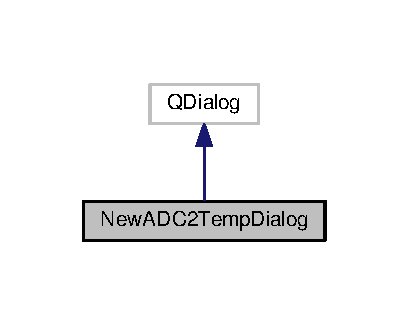
\includegraphics[width=196pt]{class_new_a_d_c2_temp_dialog__inherit__graph}
\end{center}
\end{figure}


Collaboration diagram for New\+A\+D\+C2\+Temp\+Dialog\+:\nopagebreak
\begin{figure}[H]
\begin{center}
\leavevmode
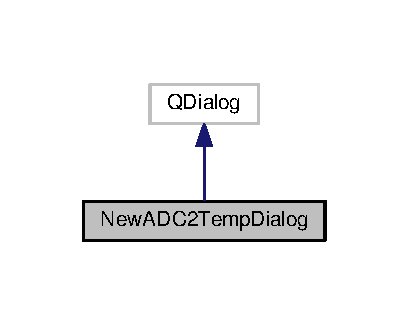
\includegraphics[width=196pt]{class_new_a_d_c2_temp_dialog__coll__graph}
\end{center}
\end{figure}
\subsection*{Public Slots}
\begin{DoxyCompactItemize}
\item 
void \hyperlink{class_new_a_d_c2_temp_dialog_aecb2c340ccb0c4ceb395ba688c092317}{Slot\+Select\+File} ()
\begin{DoxyCompactList}\small\item\em Call it to specify target file (\+\_\+filepath) \end{DoxyCompactList}\item 
void \hyperlink{class_new_a_d_c2_temp_dialog_a59b42efcbe03d9429250558eebaf6dd3}{Slot\+Save\+Settings} ()
\begin{DoxyCompactList}\small\item\em Call it to save settings into new \+\_\+filepath file. \end{DoxyCompactList}\item 
void \hyperlink{class_new_a_d_c2_temp_dialog_afe68e82283f8cf518d6df9fafcea2a43}{Slot\+Check\+Requirements} ()
\begin{DoxyCompactList}\small\item\em Checks if we have \+\_\+filepath and description specified. If yes -\/ enables Create button, otherwise -\/ disables it. \end{DoxyCompactList}\end{DoxyCompactItemize}
\subsection*{Public Member Functions}
\begin{DoxyCompactItemize}
\item 
\mbox{\Hypertarget{class_new_a_d_c2_temp_dialog_a4c7f66049c9ac670cb577700fde06eac}\label{class_new_a_d_c2_temp_dialog_a4c7f66049c9ac670cb577700fde06eac}} 
{\bfseries New\+A\+D\+C2\+Temp\+Dialog} (Q\+Widget $\ast$parent=0)
\end{DoxyCompactItemize}
\subsection*{Protected Member Functions}
\begin{DoxyCompactItemize}
\item 
\mbox{\Hypertarget{class_new_a_d_c2_temp_dialog_ad134682522a39b4843feae7662574ace}\label{class_new_a_d_c2_temp_dialog_ad134682522a39b4843feae7662574ace}} 
void {\bfseries change\+Event} (Q\+Event $\ast$e)
\end{DoxyCompactItemize}


\subsection{Detailed Description}


Definition at line 39 of file New\+A\+D\+C2\+Temp\+Dialog.\+hpp.



\subsection{Member Function Documentation}
\mbox{\Hypertarget{class_new_a_d_c2_temp_dialog_afe68e82283f8cf518d6df9fafcea2a43}\label{class_new_a_d_c2_temp_dialog_afe68e82283f8cf518d6df9fafcea2a43}} 
\index{New\+A\+D\+C2\+Temp\+Dialog@{New\+A\+D\+C2\+Temp\+Dialog}!Slot\+Check\+Requirements@{Slot\+Check\+Requirements}}
\index{Slot\+Check\+Requirements@{Slot\+Check\+Requirements}!New\+A\+D\+C2\+Temp\+Dialog@{New\+A\+D\+C2\+Temp\+Dialog}}
\subsubsection{\texorpdfstring{Slot\+Check\+Requirements}{SlotCheckRequirements}}
{\footnotesize\ttfamily void New\+A\+D\+C2\+Temp\+Dialog\+::\+Slot\+Check\+Requirements (\begin{DoxyParamCaption}{ }\end{DoxyParamCaption})\hspace{0.3cm}{\ttfamily [slot]}}



Checks if we have \+\_\+filepath and description specified. If yes -\/ enables Create button, otherwise -\/ disables it. 

Checks if we have filepath and description specified. If yes -\/ enables Create button, otherwise -\/ disables it. 

Definition at line 86 of file New\+A\+D\+C2\+Temp\+Dialog.\+cpp.

\mbox{\Hypertarget{class_new_a_d_c2_temp_dialog_a59b42efcbe03d9429250558eebaf6dd3}\label{class_new_a_d_c2_temp_dialog_a59b42efcbe03d9429250558eebaf6dd3}} 
\index{New\+A\+D\+C2\+Temp\+Dialog@{New\+A\+D\+C2\+Temp\+Dialog}!Slot\+Save\+Settings@{Slot\+Save\+Settings}}
\index{Slot\+Save\+Settings@{Slot\+Save\+Settings}!New\+A\+D\+C2\+Temp\+Dialog@{New\+A\+D\+C2\+Temp\+Dialog}}
\subsubsection{\texorpdfstring{Slot\+Save\+Settings}{SlotSaveSettings}}
{\footnotesize\ttfamily void New\+A\+D\+C2\+Temp\+Dialog\+::\+Slot\+Save\+Settings (\begin{DoxyParamCaption}{ }\end{DoxyParamCaption})\hspace{0.3cm}{\ttfamily [slot]}}



Call it to save settings into new \+\_\+filepath file. 

Call it to save settings into new filepath file. 

Definition at line 70 of file New\+A\+D\+C2\+Temp\+Dialog.\+cpp.

\mbox{\Hypertarget{class_new_a_d_c2_temp_dialog_aecb2c340ccb0c4ceb395ba688c092317}\label{class_new_a_d_c2_temp_dialog_aecb2c340ccb0c4ceb395ba688c092317}} 
\index{New\+A\+D\+C2\+Temp\+Dialog@{New\+A\+D\+C2\+Temp\+Dialog}!Slot\+Select\+File@{Slot\+Select\+File}}
\index{Slot\+Select\+File@{Slot\+Select\+File}!New\+A\+D\+C2\+Temp\+Dialog@{New\+A\+D\+C2\+Temp\+Dialog}}
\subsubsection{\texorpdfstring{Slot\+Select\+File}{SlotSelectFile}}
{\footnotesize\ttfamily void New\+A\+D\+C2\+Temp\+Dialog\+::\+Slot\+Select\+File (\begin{DoxyParamCaption}{ }\end{DoxyParamCaption})\hspace{0.3cm}{\ttfamily [slot]}}



Call it to specify target file (\+\_\+filepath) 

Call it to specify target file (filepath) 

Definition at line 59 of file New\+A\+D\+C2\+Temp\+Dialog.\+cpp.



The documentation for this class was generated from the following files\+:\begin{DoxyCompactItemize}
\item 
New\+A\+D\+C2\+Temp\+Dialog.\+hpp\item 
New\+A\+D\+C2\+Temp\+Dialog.\+cpp\end{DoxyCompactItemize}

\hypertarget{class_fossa_1_1_q_simple_graph_1_1_q_simple_graph}{}\section{Fossa\+:\+:Q\+Simple\+Graph\+:\+:Q\+Simple\+Graph Class Reference}
\label{class_fossa_1_1_q_simple_graph_1_1_q_simple_graph}\index{Fossa\+::\+Q\+Simple\+Graph\+::\+Q\+Simple\+Graph@{Fossa\+::\+Q\+Simple\+Graph\+::\+Q\+Simple\+Graph}}


\hyperlink{class_fossa_1_1_q_simple_graph_1_1_q_simple_graph}{Q\+Simple\+Graph} widget implementation.  




{\ttfamily \#include $<$Q\+Simple\+Graph.\+hpp$>$}



Inheritance diagram for Fossa\+:\+:Q\+Simple\+Graph\+:\+:Q\+Simple\+Graph\+:\nopagebreak
\begin{figure}[H]
\begin{center}
\leavevmode
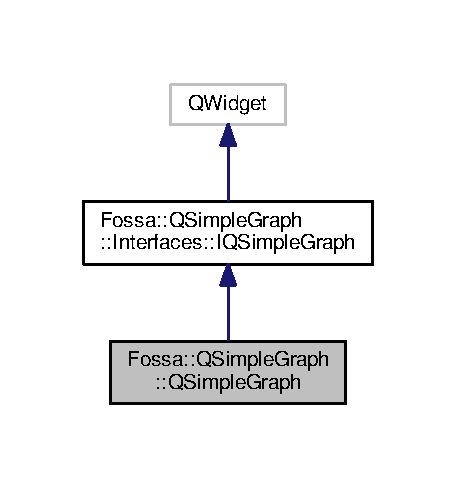
\includegraphics[width=219pt]{class_fossa_1_1_q_simple_graph_1_1_q_simple_graph__inherit__graph}
\end{center}
\end{figure}


Collaboration diagram for Fossa\+:\+:Q\+Simple\+Graph\+:\+:Q\+Simple\+Graph\+:\nopagebreak
\begin{figure}[H]
\begin{center}
\leavevmode
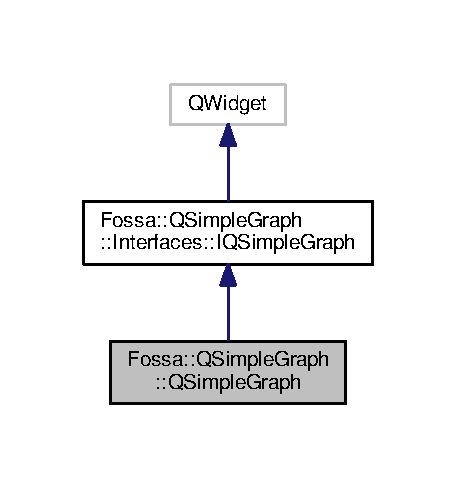
\includegraphics[width=219pt]{class_fossa_1_1_q_simple_graph_1_1_q_simple_graph__coll__graph}
\end{center}
\end{figure}
\subsection*{Public Member Functions}
\begin{DoxyCompactItemize}
\item 
\hyperlink{class_fossa_1_1_q_simple_graph_1_1_q_simple_graph_ab08b1293b3698e1e179a8d36dc737c77}{Q\+Simple\+Graph} (Q\+Widget $\ast$parent=0)
\begin{DoxyCompactList}\small\item\em \hyperlink{class_fossa_1_1_q_simple_graph_1_1_q_simple_graph}{Q\+Simple\+Graph} widget constructor. \end{DoxyCompactList}\item 
Q\+Size \hyperlink{class_fossa_1_1_q_simple_graph_1_1_q_simple_graph_a7cc7465f2137a1d9f80425afec47faeb}{size\+Hint} () const
\begin{DoxyCompactList}\small\item\em Returning hint about widget size, actually -\/ preferred size. \end{DoxyCompactList}\item 
Q\+Size \hyperlink{class_fossa_1_1_q_simple_graph_1_1_q_simple_graph_a2b427ee7fc54efd87a33d0a23bbdd1f8}{minimum\+Size\+Hint} () const
\begin{DoxyCompactList}\small\item\em Returns minimal possible widget size. \end{DoxyCompactList}\item 
void \hyperlink{class_fossa_1_1_q_simple_graph_1_1_q_simple_graph_a0eef21e58d8c85f6083d73857f871639}{Set\+Min\+X\+Value} (double min\+Value)
\begin{DoxyCompactList}\small\item\em See Set\+Max\+X\+Value for details, it have completely the same behaviour. \end{DoxyCompactList}\item 
void \hyperlink{class_fossa_1_1_q_simple_graph_1_1_q_simple_graph_a568a2dea4e0307b6888aaa048b4da97a}{Set\+Max\+X\+Value} (double max\+Value)
\begin{DoxyCompactList}\small\item\em Call it to set maximal value of X-\/axis. Please note, that if new point added to graph later, and point\textquotesingle{}s X coordinate exceeds maximal X value, then maximal X value will be increased, allowing graph to display such points. \end{DoxyCompactList}\item 
void \hyperlink{class_fossa_1_1_q_simple_graph_1_1_q_simple_graph_a8bf9aac5856a659eb89abffca7750df0}{Set\+Min\+Y\+Value} (double min\+Value)
\begin{DoxyCompactList}\small\item\em As Set\+Min\+X\+Value, but for Y-\/axis. \end{DoxyCompactList}\item 
void \hyperlink{class_fossa_1_1_q_simple_graph_1_1_q_simple_graph_a6cb6eee80dc489f300e32263833cf1cd}{Set\+Max\+Y\+Value} (double max\+Value)
\begin{DoxyCompactList}\small\item\em As Set\+Max\+X\+Value, but for Y-\/axis. \end{DoxyCompactList}\item 
void \hyperlink{class_fossa_1_1_q_simple_graph_1_1_q_simple_graph_a7579da572b54d43ccec3d2bd572b6cfa}{Set\+X\+Axis\+Title} (Q\+String title)
\begin{DoxyCompactList}\small\item\em Set title of X-\/\+Axis. \end{DoxyCompactList}\item 
void \hyperlink{class_fossa_1_1_q_simple_graph_1_1_q_simple_graph_a41c9e9d34744f6e6550ca97dc0d2f488}{Set\+Y\+Axis\+Title} (Q\+String title)
\begin{DoxyCompactList}\small\item\em As \hyperlink{class_fossa_1_1_q_simple_graph_1_1_q_simple_graph_a7579da572b54d43ccec3d2bd572b6cfa}{Set\+X\+Axis\+Title()}, but for Y-\/\+Axis. \end{DoxyCompactList}\item 
\mbox{\Hypertarget{class_fossa_1_1_q_simple_graph_1_1_q_simple_graph_a96233ee152a35d27d6b0a66712f52011}\label{class_fossa_1_1_q_simple_graph_1_1_q_simple_graph_a96233ee152a35d27d6b0a66712f52011}} 
void \hyperlink{class_fossa_1_1_q_simple_graph_1_1_q_simple_graph_a96233ee152a35d27d6b0a66712f52011}{Clear\+All\+Points} ()
\begin{DoxyCompactList}\small\item\em Removes all points from graph. \end{DoxyCompactList}\item 
void \hyperlink{class_fossa_1_1_q_simple_graph_1_1_q_simple_graph_a39fdbd2aa624b7b086b5761308d8d49c}{Add\+Point} (double X\+Val, double Y\+Val)
\begin{DoxyCompactList}\small\item\em Adds point with given X and Y value to graph. Points collection inside the graph must be self-\/ordered, so points can be added in arbitraty order. If point outside maximal and minimal values for graph, minimal and maximal values will be expanded to allow display all points. \end{DoxyCompactList}\end{DoxyCompactItemize}
\subsection*{Protected Member Functions}
\begin{DoxyCompactItemize}
\item 
void \hyperlink{class_fossa_1_1_q_simple_graph_1_1_q_simple_graph_a6559739099820e1303c1dbe2c5757bc4}{paint\+Event} (Q\+Paint\+Event $\ast$event)
\begin{DoxyCompactList}\small\item\em Painting method, paints the entrie graph. \end{DoxyCompactList}\item 
void \hyperlink{class_fossa_1_1_q_simple_graph_1_1_q_simple_graph_a7ae9773902324fc533f0b18294f7c516}{mouse\+Move\+Event} (Q\+Mouse\+Event $\ast$event)
\begin{DoxyCompactList}\small\item\em Called when mouse is being moved. \end{DoxyCompactList}\end{DoxyCompactItemize}


\subsection{Detailed Description}
\hyperlink{class_fossa_1_1_q_simple_graph_1_1_q_simple_graph}{Q\+Simple\+Graph} widget implementation. 

Definition at line 39 of file Q\+Simple\+Graph.\+hpp.



\subsection{Constructor \& Destructor Documentation}
\mbox{\Hypertarget{class_fossa_1_1_q_simple_graph_1_1_q_simple_graph_ab08b1293b3698e1e179a8d36dc737c77}\label{class_fossa_1_1_q_simple_graph_1_1_q_simple_graph_ab08b1293b3698e1e179a8d36dc737c77}} 
\index{Fossa\+::\+Q\+Simple\+Graph\+::\+Q\+Simple\+Graph@{Fossa\+::\+Q\+Simple\+Graph\+::\+Q\+Simple\+Graph}!Q\+Simple\+Graph@{Q\+Simple\+Graph}}
\index{Q\+Simple\+Graph@{Q\+Simple\+Graph}!Fossa\+::\+Q\+Simple\+Graph\+::\+Q\+Simple\+Graph@{Fossa\+::\+Q\+Simple\+Graph\+::\+Q\+Simple\+Graph}}
\subsubsection{\texorpdfstring{Q\+Simple\+Graph()}{QSimpleGraph()}}
{\footnotesize\ttfamily Fossa\+::\+Q\+Simple\+Graph\+::\+Q\+Simple\+Graph\+::\+Q\+Simple\+Graph (\begin{DoxyParamCaption}\item[{Q\+Widget $\ast$}]{parent = {\ttfamily 0} }\end{DoxyParamCaption})}



\hyperlink{class_fossa_1_1_q_simple_graph_1_1_q_simple_graph}{Q\+Simple\+Graph} widget constructor. 


\begin{DoxyParams}{Parameters}
{\em parent} & Parent widget. \\
\hline
\end{DoxyParams}


Definition at line 7 of file Q\+Simple\+Graph.\+cpp.



\subsection{Member Function Documentation}
\mbox{\Hypertarget{class_fossa_1_1_q_simple_graph_1_1_q_simple_graph_a39fdbd2aa624b7b086b5761308d8d49c}\label{class_fossa_1_1_q_simple_graph_1_1_q_simple_graph_a39fdbd2aa624b7b086b5761308d8d49c}} 
\index{Fossa\+::\+Q\+Simple\+Graph\+::\+Q\+Simple\+Graph@{Fossa\+::\+Q\+Simple\+Graph\+::\+Q\+Simple\+Graph}!Add\+Point@{Add\+Point}}
\index{Add\+Point@{Add\+Point}!Fossa\+::\+Q\+Simple\+Graph\+::\+Q\+Simple\+Graph@{Fossa\+::\+Q\+Simple\+Graph\+::\+Q\+Simple\+Graph}}
\subsubsection{\texorpdfstring{Add\+Point()}{AddPoint()}}
{\footnotesize\ttfamily void Fossa\+::\+Q\+Simple\+Graph\+::\+Q\+Simple\+Graph\+::\+Add\+Point (\begin{DoxyParamCaption}\item[{double}]{X\+Val,  }\item[{double}]{Y\+Val }\end{DoxyParamCaption})\hspace{0.3cm}{\ttfamily [virtual]}}



Adds point with given X and Y value to graph. Points collection inside the graph must be self-\/ordered, so points can be added in arbitraty order. If point outside maximal and minimal values for graph, minimal and maximal values will be expanded to allow display all points. 


\begin{DoxyParams}{Parameters}
{\em X\+Val} & X-\/axis value. \\
\hline
{\em Y\+Val} & Y-\/axis value. \\
\hline
\end{DoxyParams}


Implements \hyperlink{class_fossa_1_1_q_simple_graph_1_1_interfaces_1_1_i_q_simple_graph_a5d43e4e0f06bedb1734e4240070fe229}{Fossa\+::\+Q\+Simple\+Graph\+::\+Interfaces\+::\+I\+Q\+Simple\+Graph}.



Definition at line 322 of file Q\+Simple\+Graph.\+cpp.

\mbox{\Hypertarget{class_fossa_1_1_q_simple_graph_1_1_q_simple_graph_a2b427ee7fc54efd87a33d0a23bbdd1f8}\label{class_fossa_1_1_q_simple_graph_1_1_q_simple_graph_a2b427ee7fc54efd87a33d0a23bbdd1f8}} 
\index{Fossa\+::\+Q\+Simple\+Graph\+::\+Q\+Simple\+Graph@{Fossa\+::\+Q\+Simple\+Graph\+::\+Q\+Simple\+Graph}!minimum\+Size\+Hint@{minimum\+Size\+Hint}}
\index{minimum\+Size\+Hint@{minimum\+Size\+Hint}!Fossa\+::\+Q\+Simple\+Graph\+::\+Q\+Simple\+Graph@{Fossa\+::\+Q\+Simple\+Graph\+::\+Q\+Simple\+Graph}}
\subsubsection{\texorpdfstring{minimum\+Size\+Hint()}{minimumSizeHint()}}
{\footnotesize\ttfamily Q\+Size Fossa\+::\+Q\+Simple\+Graph\+::\+Q\+Simple\+Graph\+::minimum\+Size\+Hint (\begin{DoxyParamCaption}{ }\end{DoxyParamCaption}) const}



Returns minimal possible widget size. 

\begin{DoxyReturn}{Returns}
Minimal possible widget size. 
\end{DoxyReturn}


Definition at line 15 of file Q\+Simple\+Graph.\+cpp.

\mbox{\Hypertarget{class_fossa_1_1_q_simple_graph_1_1_q_simple_graph_a7ae9773902324fc533f0b18294f7c516}\label{class_fossa_1_1_q_simple_graph_1_1_q_simple_graph_a7ae9773902324fc533f0b18294f7c516}} 
\index{Fossa\+::\+Q\+Simple\+Graph\+::\+Q\+Simple\+Graph@{Fossa\+::\+Q\+Simple\+Graph\+::\+Q\+Simple\+Graph}!mouse\+Move\+Event@{mouse\+Move\+Event}}
\index{mouse\+Move\+Event@{mouse\+Move\+Event}!Fossa\+::\+Q\+Simple\+Graph\+::\+Q\+Simple\+Graph@{Fossa\+::\+Q\+Simple\+Graph\+::\+Q\+Simple\+Graph}}
\subsubsection{\texorpdfstring{mouse\+Move\+Event()}{mouseMoveEvent()}}
{\footnotesize\ttfamily void Fossa\+::\+Q\+Simple\+Graph\+::\+Q\+Simple\+Graph\+::mouse\+Move\+Event (\begin{DoxyParamCaption}\item[{Q\+Mouse\+Event $\ast$}]{event }\end{DoxyParamCaption})\hspace{0.3cm}{\ttfamily [protected]}}



Called when mouse is being moved. 


\begin{DoxyParams}{Parameters}
{\em event} & Mouse move parameters. \\
\hline
\end{DoxyParams}


Definition at line 25 of file Q\+Simple\+Graph.\+cpp.

\mbox{\Hypertarget{class_fossa_1_1_q_simple_graph_1_1_q_simple_graph_a6559739099820e1303c1dbe2c5757bc4}\label{class_fossa_1_1_q_simple_graph_1_1_q_simple_graph_a6559739099820e1303c1dbe2c5757bc4}} 
\index{Fossa\+::\+Q\+Simple\+Graph\+::\+Q\+Simple\+Graph@{Fossa\+::\+Q\+Simple\+Graph\+::\+Q\+Simple\+Graph}!paint\+Event@{paint\+Event}}
\index{paint\+Event@{paint\+Event}!Fossa\+::\+Q\+Simple\+Graph\+::\+Q\+Simple\+Graph@{Fossa\+::\+Q\+Simple\+Graph\+::\+Q\+Simple\+Graph}}
\subsubsection{\texorpdfstring{paint\+Event()}{paintEvent()}}
{\footnotesize\ttfamily void Fossa\+::\+Q\+Simple\+Graph\+::\+Q\+Simple\+Graph\+::paint\+Event (\begin{DoxyParamCaption}\item[{Q\+Paint\+Event $\ast$}]{event }\end{DoxyParamCaption})\hspace{0.3cm}{\ttfamily [protected]}}



Painting method, paints the entrie graph. 


\begin{DoxyParams}{Parameters}
{\em event} & Pointer to paint event. \\
\hline
\end{DoxyParams}


Definition at line 43 of file Q\+Simple\+Graph.\+cpp.

\mbox{\Hypertarget{class_fossa_1_1_q_simple_graph_1_1_q_simple_graph_a568a2dea4e0307b6888aaa048b4da97a}\label{class_fossa_1_1_q_simple_graph_1_1_q_simple_graph_a568a2dea4e0307b6888aaa048b4da97a}} 
\index{Fossa\+::\+Q\+Simple\+Graph\+::\+Q\+Simple\+Graph@{Fossa\+::\+Q\+Simple\+Graph\+::\+Q\+Simple\+Graph}!Set\+Max\+X\+Value@{Set\+Max\+X\+Value}}
\index{Set\+Max\+X\+Value@{Set\+Max\+X\+Value}!Fossa\+::\+Q\+Simple\+Graph\+::\+Q\+Simple\+Graph@{Fossa\+::\+Q\+Simple\+Graph\+::\+Q\+Simple\+Graph}}
\subsubsection{\texorpdfstring{Set\+Max\+X\+Value()}{SetMaxXValue()}}
{\footnotesize\ttfamily void Fossa\+::\+Q\+Simple\+Graph\+::\+Q\+Simple\+Graph\+::\+Set\+Max\+X\+Value (\begin{DoxyParamCaption}\item[{double}]{max\+Value }\end{DoxyParamCaption})\hspace{0.3cm}{\ttfamily [virtual]}}



Call it to set maximal value of X-\/axis. Please note, that if new point added to graph later, and point\textquotesingle{}s X coordinate exceeds maximal X value, then maximal X value will be increased, allowing graph to display such points. 


\begin{DoxyParams}{Parameters}
{\em max\+Value} & New maximal value. If it less then minimal X value, it will be set to minimal X value. \\
\hline
\end{DoxyParams}


Implements \hyperlink{class_fossa_1_1_q_simple_graph_1_1_interfaces_1_1_i_q_simple_graph_a04e7ec46c2be46257bef53c7bf978a2a}{Fossa\+::\+Q\+Simple\+Graph\+::\+Interfaces\+::\+I\+Q\+Simple\+Graph}.



Definition at line 259 of file Q\+Simple\+Graph.\+cpp.

\mbox{\Hypertarget{class_fossa_1_1_q_simple_graph_1_1_q_simple_graph_a6cb6eee80dc489f300e32263833cf1cd}\label{class_fossa_1_1_q_simple_graph_1_1_q_simple_graph_a6cb6eee80dc489f300e32263833cf1cd}} 
\index{Fossa\+::\+Q\+Simple\+Graph\+::\+Q\+Simple\+Graph@{Fossa\+::\+Q\+Simple\+Graph\+::\+Q\+Simple\+Graph}!Set\+Max\+Y\+Value@{Set\+Max\+Y\+Value}}
\index{Set\+Max\+Y\+Value@{Set\+Max\+Y\+Value}!Fossa\+::\+Q\+Simple\+Graph\+::\+Q\+Simple\+Graph@{Fossa\+::\+Q\+Simple\+Graph\+::\+Q\+Simple\+Graph}}
\subsubsection{\texorpdfstring{Set\+Max\+Y\+Value()}{SetMaxYValue()}}
{\footnotesize\ttfamily void Fossa\+::\+Q\+Simple\+Graph\+::\+Q\+Simple\+Graph\+::\+Set\+Max\+Y\+Value (\begin{DoxyParamCaption}\item[{double}]{max\+Value }\end{DoxyParamCaption})\hspace{0.3cm}{\ttfamily [virtual]}}



As Set\+Max\+X\+Value, but for Y-\/axis. 


\begin{DoxyParams}{Parameters}
{\em max\+Value} & See Set\+Max\+X\+Value. \\
\hline
\end{DoxyParams}


Implements \hyperlink{class_fossa_1_1_q_simple_graph_1_1_interfaces_1_1_i_q_simple_graph_a09e04c116810e79ca1663d2075477746}{Fossa\+::\+Q\+Simple\+Graph\+::\+Interfaces\+::\+I\+Q\+Simple\+Graph}.



Definition at line 271 of file Q\+Simple\+Graph.\+cpp.

\mbox{\Hypertarget{class_fossa_1_1_q_simple_graph_1_1_q_simple_graph_a0eef21e58d8c85f6083d73857f871639}\label{class_fossa_1_1_q_simple_graph_1_1_q_simple_graph_a0eef21e58d8c85f6083d73857f871639}} 
\index{Fossa\+::\+Q\+Simple\+Graph\+::\+Q\+Simple\+Graph@{Fossa\+::\+Q\+Simple\+Graph\+::\+Q\+Simple\+Graph}!Set\+Min\+X\+Value@{Set\+Min\+X\+Value}}
\index{Set\+Min\+X\+Value@{Set\+Min\+X\+Value}!Fossa\+::\+Q\+Simple\+Graph\+::\+Q\+Simple\+Graph@{Fossa\+::\+Q\+Simple\+Graph\+::\+Q\+Simple\+Graph}}
\subsubsection{\texorpdfstring{Set\+Min\+X\+Value()}{SetMinXValue()}}
{\footnotesize\ttfamily void Fossa\+::\+Q\+Simple\+Graph\+::\+Q\+Simple\+Graph\+::\+Set\+Min\+X\+Value (\begin{DoxyParamCaption}\item[{double}]{min\+Value }\end{DoxyParamCaption})\hspace{0.3cm}{\ttfamily [virtual]}}



See Set\+Max\+X\+Value for details, it have completely the same behaviour. 


\begin{DoxyParams}{Parameters}
{\em min\+Value} & New minimal value. If it greater then maximal X value, it will be set to maximal X value. \\
\hline
\end{DoxyParams}


Implements \hyperlink{class_fossa_1_1_q_simple_graph_1_1_interfaces_1_1_i_q_simple_graph_a4266725f87b306e572ad1ae37cfab4ef}{Fossa\+::\+Q\+Simple\+Graph\+::\+Interfaces\+::\+I\+Q\+Simple\+Graph}.



Definition at line 253 of file Q\+Simple\+Graph.\+cpp.

\mbox{\Hypertarget{class_fossa_1_1_q_simple_graph_1_1_q_simple_graph_a8bf9aac5856a659eb89abffca7750df0}\label{class_fossa_1_1_q_simple_graph_1_1_q_simple_graph_a8bf9aac5856a659eb89abffca7750df0}} 
\index{Fossa\+::\+Q\+Simple\+Graph\+::\+Q\+Simple\+Graph@{Fossa\+::\+Q\+Simple\+Graph\+::\+Q\+Simple\+Graph}!Set\+Min\+Y\+Value@{Set\+Min\+Y\+Value}}
\index{Set\+Min\+Y\+Value@{Set\+Min\+Y\+Value}!Fossa\+::\+Q\+Simple\+Graph\+::\+Q\+Simple\+Graph@{Fossa\+::\+Q\+Simple\+Graph\+::\+Q\+Simple\+Graph}}
\subsubsection{\texorpdfstring{Set\+Min\+Y\+Value()}{SetMinYValue()}}
{\footnotesize\ttfamily void Fossa\+::\+Q\+Simple\+Graph\+::\+Q\+Simple\+Graph\+::\+Set\+Min\+Y\+Value (\begin{DoxyParamCaption}\item[{double}]{min\+Value }\end{DoxyParamCaption})\hspace{0.3cm}{\ttfamily [virtual]}}



As Set\+Min\+X\+Value, but for Y-\/axis. 


\begin{DoxyParams}{Parameters}
{\em min\+Value} & See Set\+Min\+X\+Value. \\
\hline
\end{DoxyParams}


Implements \hyperlink{class_fossa_1_1_q_simple_graph_1_1_interfaces_1_1_i_q_simple_graph_a3fdd1f6b538e2dfbf4a0140acd6b6e94}{Fossa\+::\+Q\+Simple\+Graph\+::\+Interfaces\+::\+I\+Q\+Simple\+Graph}.



Definition at line 265 of file Q\+Simple\+Graph.\+cpp.

\mbox{\Hypertarget{class_fossa_1_1_q_simple_graph_1_1_q_simple_graph_a7579da572b54d43ccec3d2bd572b6cfa}\label{class_fossa_1_1_q_simple_graph_1_1_q_simple_graph_a7579da572b54d43ccec3d2bd572b6cfa}} 
\index{Fossa\+::\+Q\+Simple\+Graph\+::\+Q\+Simple\+Graph@{Fossa\+::\+Q\+Simple\+Graph\+::\+Q\+Simple\+Graph}!Set\+X\+Axis\+Title@{Set\+X\+Axis\+Title}}
\index{Set\+X\+Axis\+Title@{Set\+X\+Axis\+Title}!Fossa\+::\+Q\+Simple\+Graph\+::\+Q\+Simple\+Graph@{Fossa\+::\+Q\+Simple\+Graph\+::\+Q\+Simple\+Graph}}
\subsubsection{\texorpdfstring{Set\+X\+Axis\+Title()}{SetXAxisTitle()}}
{\footnotesize\ttfamily void Fossa\+::\+Q\+Simple\+Graph\+::\+Q\+Simple\+Graph\+::\+Set\+X\+Axis\+Title (\begin{DoxyParamCaption}\item[{Q\+String}]{title }\end{DoxyParamCaption})\hspace{0.3cm}{\ttfamily [virtual]}}



Set title of X-\/\+Axis. 


\begin{DoxyParams}{Parameters}
{\em title} & Title. \\
\hline
\end{DoxyParams}


Implements \hyperlink{class_fossa_1_1_q_simple_graph_1_1_interfaces_1_1_i_q_simple_graph_adfca7d41a47790e8403507544468ba86}{Fossa\+::\+Q\+Simple\+Graph\+::\+Interfaces\+::\+I\+Q\+Simple\+Graph}.



Definition at line 307 of file Q\+Simple\+Graph.\+cpp.

\mbox{\Hypertarget{class_fossa_1_1_q_simple_graph_1_1_q_simple_graph_a41c9e9d34744f6e6550ca97dc0d2f488}\label{class_fossa_1_1_q_simple_graph_1_1_q_simple_graph_a41c9e9d34744f6e6550ca97dc0d2f488}} 
\index{Fossa\+::\+Q\+Simple\+Graph\+::\+Q\+Simple\+Graph@{Fossa\+::\+Q\+Simple\+Graph\+::\+Q\+Simple\+Graph}!Set\+Y\+Axis\+Title@{Set\+Y\+Axis\+Title}}
\index{Set\+Y\+Axis\+Title@{Set\+Y\+Axis\+Title}!Fossa\+::\+Q\+Simple\+Graph\+::\+Q\+Simple\+Graph@{Fossa\+::\+Q\+Simple\+Graph\+::\+Q\+Simple\+Graph}}
\subsubsection{\texorpdfstring{Set\+Y\+Axis\+Title()}{SetYAxisTitle()}}
{\footnotesize\ttfamily void Fossa\+::\+Q\+Simple\+Graph\+::\+Q\+Simple\+Graph\+::\+Set\+Y\+Axis\+Title (\begin{DoxyParamCaption}\item[{Q\+String}]{title }\end{DoxyParamCaption})\hspace{0.3cm}{\ttfamily [virtual]}}



As \hyperlink{class_fossa_1_1_q_simple_graph_1_1_q_simple_graph_a7579da572b54d43ccec3d2bd572b6cfa}{Set\+X\+Axis\+Title()}, but for Y-\/\+Axis. 


\begin{DoxyParams}{Parameters}
{\em title} & See \hyperlink{class_fossa_1_1_q_simple_graph_1_1_q_simple_graph_a7579da572b54d43ccec3d2bd572b6cfa}{Set\+X\+Axis\+Title()}. \\
\hline
\end{DoxyParams}


Implements \hyperlink{class_fossa_1_1_q_simple_graph_1_1_interfaces_1_1_i_q_simple_graph_a606c07c40ed294cdd568de5488875af5}{Fossa\+::\+Q\+Simple\+Graph\+::\+Interfaces\+::\+I\+Q\+Simple\+Graph}.



Definition at line 312 of file Q\+Simple\+Graph.\+cpp.

\mbox{\Hypertarget{class_fossa_1_1_q_simple_graph_1_1_q_simple_graph_a7cc7465f2137a1d9f80425afec47faeb}\label{class_fossa_1_1_q_simple_graph_1_1_q_simple_graph_a7cc7465f2137a1d9f80425afec47faeb}} 
\index{Fossa\+::\+Q\+Simple\+Graph\+::\+Q\+Simple\+Graph@{Fossa\+::\+Q\+Simple\+Graph\+::\+Q\+Simple\+Graph}!size\+Hint@{size\+Hint}}
\index{size\+Hint@{size\+Hint}!Fossa\+::\+Q\+Simple\+Graph\+::\+Q\+Simple\+Graph@{Fossa\+::\+Q\+Simple\+Graph\+::\+Q\+Simple\+Graph}}
\subsubsection{\texorpdfstring{size\+Hint()}{sizeHint()}}
{\footnotesize\ttfamily Q\+Size Fossa\+::\+Q\+Simple\+Graph\+::\+Q\+Simple\+Graph\+::size\+Hint (\begin{DoxyParamCaption}{ }\end{DoxyParamCaption}) const}



Returning hint about widget size, actually -\/ preferred size. 

\begin{DoxyReturn}{Returns}
Q\+Size with hint about widget size. 
\end{DoxyReturn}


Definition at line 20 of file Q\+Simple\+Graph.\+cpp.



The documentation for this class was generated from the following files\+:\begin{DoxyCompactItemize}
\item 
Fossas\+Simple\+Graph/\+Implementations/Q\+Simple\+Graph.\+hpp\item 
Fossas\+Simple\+Graph/\+Implementations/Q\+Simple\+Graph.\+cpp\end{DoxyCompactItemize}

\hypertarget{class_settings_generator}{}\section{Settings\+Generator Class Reference}
\label{class_settings_generator}\index{Settings\+Generator@{Settings\+Generator}}


Class, being used to generate settings (see Interfaces/\+I\+Settings\+Generator for information)  




{\ttfamily \#include $<$Settings\+Generator.\+hpp$>$}



Inheritance diagram for Settings\+Generator\+:\nopagebreak
\begin{figure}[H]
\begin{center}
\leavevmode
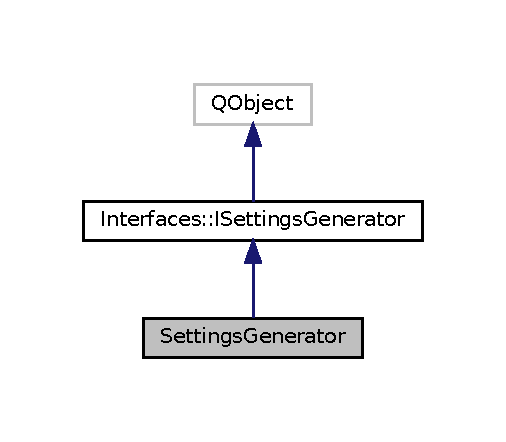
\includegraphics[width=228pt]{class_settings_generator__inherit__graph}
\end{center}
\end{figure}


Collaboration diagram for Settings\+Generator\+:\nopagebreak
\begin{figure}[H]
\begin{center}
\leavevmode
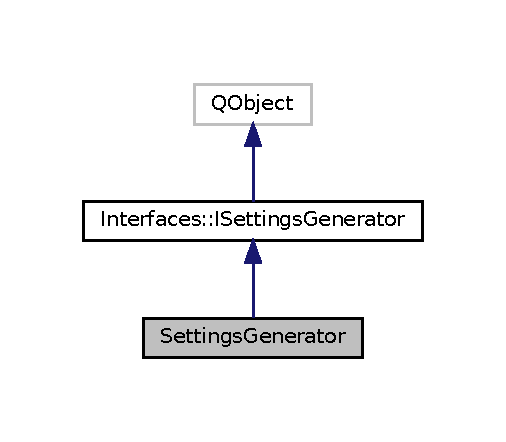
\includegraphics[width=228pt]{class_settings_generator__coll__graph}
\end{center}
\end{figure}
\subsection*{Public Member Functions}
\begin{DoxyCompactItemize}
\item 
\hyperlink{class_settings_generator_a063e189547011b62a567ff55446341d7}{Settings\+Generator} (\hyperlink{class_interfaces_1_1_i_adc_temperature_convertor}{Interfaces\+::\+I\+Adc\+Temperature\+Convertor} $\ast$convertor)
\begin{DoxyCompactList}\small\item\em Constructor. Initializes steps list, default base temperature and so on. \end{DoxyCompactList}\item 
\mbox{\Hypertarget{class_settings_generator_aeb8e3d3875929a6869aa93552f30599f}\label{class_settings_generator_aeb8e3d3875929a6869aa93552f30599f}} 
\hyperlink{class_settings_generator_aeb8e3d3875929a6869aa93552f30599f}{$\sim$\+Settings\+Generator} ()
\begin{DoxyCompactList}\small\item\em Destructor. \end{DoxyCompactList}\item 
void \hyperlink{class_settings_generator_a84b81d11cb5f83d4066e73a03acfc143}{Initialize\+Steps\+List} (uint steps\+\_\+number)
\begin{DoxyCompactList}\small\item\em Call this method to initialize steps list. It must be called before any other methods. Implementation must be ready to provide the instance of I\+Adc\+Temperature\+Convertor to steps. \end{DoxyCompactList}\item 
void \hyperlink{class_settings_generator_aed9e7acb30bfd559b1ac70ceeddd8973}{Set\+Base\+Temperature} (double btemp)
\begin{DoxyCompactList}\small\item\em Set\+Base\+Temperature -\/ Call it to set base temperature (in Celsius). Please note, that all steps will be recalculated afterwards. \end{DoxyCompactList}\item 
double \hyperlink{class_settings_generator_a80b1ff8060a16d149989d98a88ab253e}{Get\+Base\+Temperature} ()
\begin{DoxyCompactList}\small\item\em Get\+Base\+Temperature -\/ Call it to get base temperature (in Celsius). Please note, that base temperature returned by this method M\+AY D\+I\+F\+F\+ER from that, what was set by \hyperlink{class_settings_generator_aed9e7acb30bfd559b1ac70ceeddd8973}{Set\+Base\+Temperature()}. It is because implementation may store A\+DC value rather than temperature. \end{DoxyCompactList}\item 
uint \hyperlink{class_settings_generator_a5f3f78597f001c127b89f6447a46df09}{Get\+Base\+Temperature\+A\+DC} ()
\begin{DoxyCompactList}\small\item\em Get\+Base\+Temperature\+A\+DC Like \hyperlink{class_settings_generator_a80b1ff8060a16d149989d98a88ab253e}{Get\+Base\+Temperature()}, but returns A\+DC code for it. \end{DoxyCompactList}\item 
void \hyperlink{class_settings_generator_a1c1960b9021f7081b4c42c4d7c0eda34}{Set\+Base\+R\+PM} (uint base\+\_\+rpm)
\begin{DoxyCompactList}\small\item\em Set\+Base\+Rpm Call this method to set base R\+PM. Base R\+PM -\/ is a R\+PM at base temperature. Please note, that all steps will be recalculated afterwards. \end{DoxyCompactList}\item 
uint \hyperlink{class_settings_generator_a99bbe6e67e638ccc7bf6b21b3bc36135}{Get\+Base\+R\+PM} ()
\begin{DoxyCompactList}\small\item\em Get\+Base\+R\+PM -\/ Returns base R\+PM level. See \hyperlink{class_settings_generator_a1c1960b9021f7081b4c42c4d7c0eda34}{Set\+Base\+R\+P\+M()} for details. \end{DoxyCompactList}\item 
\mbox{\Hypertarget{class_settings_generator_a7c9c1a7a3928ba3ce0ad110593b97a96}\label{class_settings_generator_a7c9c1a7a3928ba3ce0ad110593b97a96}} 
void \hyperlink{class_settings_generator_a7c9c1a7a3928ba3ce0ad110593b97a96}{Calculate\+Steps} ()
\begin{DoxyCompactList}\small\item\em Calculate\+Steps Call this method to recalculate step A\+DC levels and R\+P\+Ms. \end{DoxyCompactList}\item 
\hyperlink{class_interfaces_1_1_i_settings_step}{Interfaces\+::\+I\+Settings\+Step} $\ast$ \hyperlink{class_settings_generator_a37f4175a0ed24853b2f187f15505086b}{Get\+Step\+Ptr} (uint step)
\begin{DoxyCompactList}\small\item\em Returns pointer to step with given number to allow manipulations with step. Don\textquotesingle{}t forget to call \hyperlink{class_settings_generator_a7c9c1a7a3928ba3ce0ad110593b97a96}{Calculate\+Steps()} after making any changes. \end{DoxyCompactList}\end{DoxyCompactItemize}


\subsection{Detailed Description}
Class, being used to generate settings (see Interfaces/\+I\+Settings\+Generator for information) 

Definition at line 56 of file Settings\+Generator.\+hpp.



\subsection{Constructor \& Destructor Documentation}
\mbox{\Hypertarget{class_settings_generator_a063e189547011b62a567ff55446341d7}\label{class_settings_generator_a063e189547011b62a567ff55446341d7}} 
\index{Settings\+Generator@{Settings\+Generator}!Settings\+Generator@{Settings\+Generator}}
\index{Settings\+Generator@{Settings\+Generator}!Settings\+Generator@{Settings\+Generator}}
\subsubsection{\texorpdfstring{Settings\+Generator()}{SettingsGenerator()}}
{\footnotesize\ttfamily Settings\+Generator\+::\+Settings\+Generator (\begin{DoxyParamCaption}\item[{\hyperlink{class_interfaces_1_1_i_adc_temperature_convertor}{Interfaces\+::\+I\+Adc\+Temperature\+Convertor} $\ast$}]{convertor }\end{DoxyParamCaption})}



Constructor. Initializes steps list, default base temperature and so on. 


\begin{DoxyParams}{Parameters}
{\em convertor} & -\/ Pointer to instance of \hyperlink{class_adc_temperature_convertor}{Adc\+Temperature\+Convertor} class. \\
\hline
\end{DoxyParams}


Definition at line 23 of file Settings\+Generator.\+cpp.



\subsection{Member Function Documentation}
\mbox{\Hypertarget{class_settings_generator_a99bbe6e67e638ccc7bf6b21b3bc36135}\label{class_settings_generator_a99bbe6e67e638ccc7bf6b21b3bc36135}} 
\index{Settings\+Generator@{Settings\+Generator}!Get\+Base\+R\+PM@{Get\+Base\+R\+PM}}
\index{Get\+Base\+R\+PM@{Get\+Base\+R\+PM}!Settings\+Generator@{Settings\+Generator}}
\subsubsection{\texorpdfstring{Get\+Base\+R\+P\+M()}{GetBaseRPM()}}
{\footnotesize\ttfamily uint Settings\+Generator\+::\+Get\+Base\+R\+PM (\begin{DoxyParamCaption}{ }\end{DoxyParamCaption})\hspace{0.3cm}{\ttfamily [virtual]}}



Get\+Base\+R\+PM -\/ Returns base R\+PM level. See \hyperlink{class_settings_generator_a1c1960b9021f7081b4c42c4d7c0eda34}{Set\+Base\+R\+P\+M()} for details. 

\begin{DoxyReturn}{Returns}
Base R\+PM level. 
\end{DoxyReturn}


Implements \hyperlink{class_interfaces_1_1_i_settings_generator_ad088253da57b2ee0b94fe6fd1fb2dfdd}{Interfaces\+::\+I\+Settings\+Generator}.



Definition at line 73 of file Settings\+Generator.\+cpp.

\mbox{\Hypertarget{class_settings_generator_a80b1ff8060a16d149989d98a88ab253e}\label{class_settings_generator_a80b1ff8060a16d149989d98a88ab253e}} 
\index{Settings\+Generator@{Settings\+Generator}!Get\+Base\+Temperature@{Get\+Base\+Temperature}}
\index{Get\+Base\+Temperature@{Get\+Base\+Temperature}!Settings\+Generator@{Settings\+Generator}}
\subsubsection{\texorpdfstring{Get\+Base\+Temperature()}{GetBaseTemperature()}}
{\footnotesize\ttfamily double Settings\+Generator\+::\+Get\+Base\+Temperature (\begin{DoxyParamCaption}{ }\end{DoxyParamCaption})\hspace{0.3cm}{\ttfamily [virtual]}}



Get\+Base\+Temperature -\/ Call it to get base temperature (in Celsius). Please note, that base temperature returned by this method M\+AY D\+I\+F\+F\+ER from that, what was set by \hyperlink{class_settings_generator_aed9e7acb30bfd559b1ac70ceeddd8973}{Set\+Base\+Temperature()}. It is because implementation may store A\+DC value rather than temperature. 

\begin{DoxyReturn}{Returns}
Base temperature in Celsius 
\end{DoxyReturn}


Implements \hyperlink{class_interfaces_1_1_i_settings_generator_a9cc36185b446f21e09a0e5633f39a1c5}{Interfaces\+::\+I\+Settings\+Generator}.



Definition at line 56 of file Settings\+Generator.\+cpp.

\mbox{\Hypertarget{class_settings_generator_a5f3f78597f001c127b89f6447a46df09}\label{class_settings_generator_a5f3f78597f001c127b89f6447a46df09}} 
\index{Settings\+Generator@{Settings\+Generator}!Get\+Base\+Temperature\+A\+DC@{Get\+Base\+Temperature\+A\+DC}}
\index{Get\+Base\+Temperature\+A\+DC@{Get\+Base\+Temperature\+A\+DC}!Settings\+Generator@{Settings\+Generator}}
\subsubsection{\texorpdfstring{Get\+Base\+Temperature\+A\+D\+C()}{GetBaseTemperatureADC()}}
{\footnotesize\ttfamily uint Settings\+Generator\+::\+Get\+Base\+Temperature\+A\+DC (\begin{DoxyParamCaption}{ }\end{DoxyParamCaption})\hspace{0.3cm}{\ttfamily [virtual]}}



Get\+Base\+Temperature\+A\+DC Like \hyperlink{class_settings_generator_a80b1ff8060a16d149989d98a88ab253e}{Get\+Base\+Temperature()}, but returns A\+DC code for it. 

\begin{DoxyReturn}{Returns}
A\+DC code for current base temperature. 
\end{DoxyReturn}


Implements \hyperlink{class_interfaces_1_1_i_settings_generator_a1000ff41c6eecdb55a46c859ca0ebe67}{Interfaces\+::\+I\+Settings\+Generator}.



Definition at line 61 of file Settings\+Generator.\+cpp.

\mbox{\Hypertarget{class_settings_generator_a37f4175a0ed24853b2f187f15505086b}\label{class_settings_generator_a37f4175a0ed24853b2f187f15505086b}} 
\index{Settings\+Generator@{Settings\+Generator}!Get\+Step\+Ptr@{Get\+Step\+Ptr}}
\index{Get\+Step\+Ptr@{Get\+Step\+Ptr}!Settings\+Generator@{Settings\+Generator}}
\subsubsection{\texorpdfstring{Get\+Step\+Ptr()}{GetStepPtr()}}
{\footnotesize\ttfamily \hyperlink{class_interfaces_1_1_i_settings_step}{Interfaces\+::\+I\+Settings\+Step} $\ast$ Settings\+Generator\+::\+Get\+Step\+Ptr (\begin{DoxyParamCaption}\item[{uint}]{step }\end{DoxyParamCaption})\hspace{0.3cm}{\ttfamily [virtual]}}



Returns pointer to step with given number to allow manipulations with step. Don\textquotesingle{}t forget to call \hyperlink{class_settings_generator_a7c9c1a7a3928ba3ce0ad110593b97a96}{Calculate\+Steps()} after making any changes. 


\begin{DoxyParams}{Parameters}
{\em step} & Step number \\
\hline
\end{DoxyParams}
\begin{DoxyReturn}{Returns}
Pointer to step 
\end{DoxyReturn}


Implements \hyperlink{class_interfaces_1_1_i_settings_generator_af1b65a18c3ade3235715ae2e9cdbcfe0}{Interfaces\+::\+I\+Settings\+Generator}.



Definition at line 110 of file Settings\+Generator.\+cpp.

\mbox{\Hypertarget{class_settings_generator_a84b81d11cb5f83d4066e73a03acfc143}\label{class_settings_generator_a84b81d11cb5f83d4066e73a03acfc143}} 
\index{Settings\+Generator@{Settings\+Generator}!Initialize\+Steps\+List@{Initialize\+Steps\+List}}
\index{Initialize\+Steps\+List@{Initialize\+Steps\+List}!Settings\+Generator@{Settings\+Generator}}
\subsubsection{\texorpdfstring{Initialize\+Steps\+List()}{InitializeStepsList()}}
{\footnotesize\ttfamily void Settings\+Generator\+::\+Initialize\+Steps\+List (\begin{DoxyParamCaption}\item[{uint}]{steps\+\_\+number }\end{DoxyParamCaption})\hspace{0.3cm}{\ttfamily [virtual]}}



Call this method to initialize steps list. It must be called before any other methods. Implementation must be ready to provide the instance of I\+Adc\+Temperature\+Convertor to steps. 


\begin{DoxyParams}{Parameters}
{\em steps\+\_\+number} & How many steps we have \\
\hline
\end{DoxyParams}


Implements \hyperlink{class_interfaces_1_1_i_settings_generator_a4aa0307e906c003012aad75101072c65}{Interfaces\+::\+I\+Settings\+Generator}.



Definition at line 31 of file Settings\+Generator.\+cpp.

\mbox{\Hypertarget{class_settings_generator_a1c1960b9021f7081b4c42c4d7c0eda34}\label{class_settings_generator_a1c1960b9021f7081b4c42c4d7c0eda34}} 
\index{Settings\+Generator@{Settings\+Generator}!Set\+Base\+R\+PM@{Set\+Base\+R\+PM}}
\index{Set\+Base\+R\+PM@{Set\+Base\+R\+PM}!Settings\+Generator@{Settings\+Generator}}
\subsubsection{\texorpdfstring{Set\+Base\+R\+P\+M()}{SetBaseRPM()}}
{\footnotesize\ttfamily void Settings\+Generator\+::\+Set\+Base\+R\+PM (\begin{DoxyParamCaption}\item[{uint}]{base\+\_\+rpm }\end{DoxyParamCaption})\hspace{0.3cm}{\ttfamily [virtual]}}



Set\+Base\+Rpm Call this method to set base R\+PM. Base R\+PM -\/ is a R\+PM at base temperature. Please note, that all steps will be recalculated afterwards. 


\begin{DoxyParams}{Parameters}
{\em base\+\_\+rpm} & -\/ Base R\+PM value. 0x00 -\/ cooler is stopped. 0x01 -\/ minimal possible R\+PM. 0x100 -\/ maximal possible R\+PM. \\
\hline
\end{DoxyParams}


Implements \hyperlink{class_interfaces_1_1_i_settings_generator_a4caf07447d0930440d9f21318892244c}{Interfaces\+::\+I\+Settings\+Generator}.



Definition at line 66 of file Settings\+Generator.\+cpp.

\mbox{\Hypertarget{class_settings_generator_aed9e7acb30bfd559b1ac70ceeddd8973}\label{class_settings_generator_aed9e7acb30bfd559b1ac70ceeddd8973}} 
\index{Settings\+Generator@{Settings\+Generator}!Set\+Base\+Temperature@{Set\+Base\+Temperature}}
\index{Set\+Base\+Temperature@{Set\+Base\+Temperature}!Settings\+Generator@{Settings\+Generator}}
\subsubsection{\texorpdfstring{Set\+Base\+Temperature()}{SetBaseTemperature()}}
{\footnotesize\ttfamily void Settings\+Generator\+::\+Set\+Base\+Temperature (\begin{DoxyParamCaption}\item[{double}]{btemp }\end{DoxyParamCaption})\hspace{0.3cm}{\ttfamily [virtual]}}



Set\+Base\+Temperature -\/ Call it to set base temperature (in Celsius). Please note, that all steps will be recalculated afterwards. 


\begin{DoxyParams}{Parameters}
{\em btemp} & Base temperature in Celsius \\
\hline
\end{DoxyParams}


Implements \hyperlink{class_interfaces_1_1_i_settings_generator_a8b60ba05790994db0303b251f655e95d}{Interfaces\+::\+I\+Settings\+Generator}.



Definition at line 49 of file Settings\+Generator.\+cpp.



The documentation for this class was generated from the following files\+:\begin{DoxyCompactItemize}
\item 
Implementations/Settings\+Generator.\+hpp\item 
Implementations/Settings\+Generator.\+cpp\end{DoxyCompactItemize}

\hypertarget{class_settings_saver_loader}{}\section{Settings\+Saver\+Loader Class Reference}
\label{class_settings_saver_loader}\index{Settings\+Saver\+Loader@{Settings\+Saver\+Loader}}


Class to save and load settings to X\+ML.  




{\ttfamily \#include $<$Settings\+Saver\+Loader.\+hpp$>$}



Inheritance diagram for Settings\+Saver\+Loader\+:\nopagebreak
\begin{figure}[H]
\begin{center}
\leavevmode
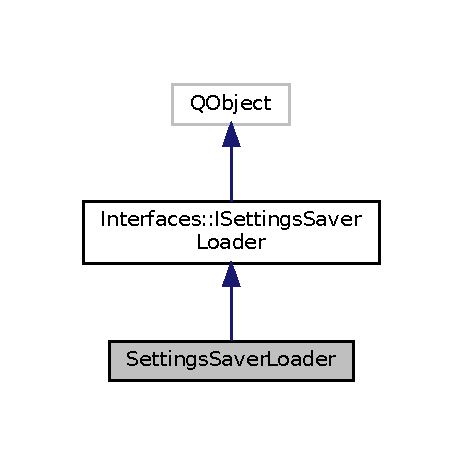
\includegraphics[width=222pt]{class_settings_saver_loader__inherit__graph}
\end{center}
\end{figure}


Collaboration diagram for Settings\+Saver\+Loader\+:\nopagebreak
\begin{figure}[H]
\begin{center}
\leavevmode
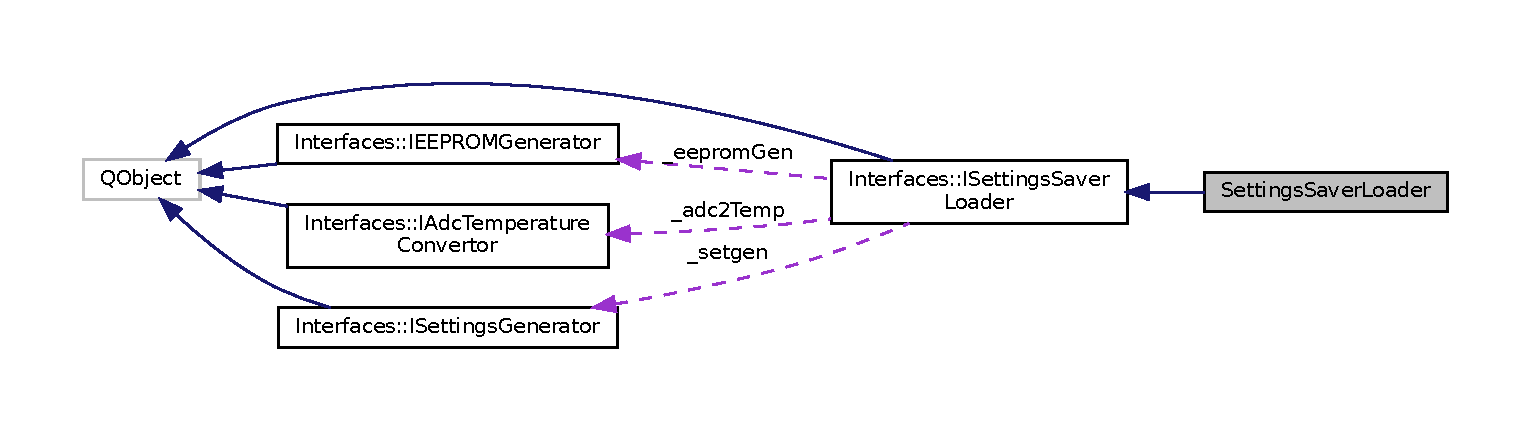
\includegraphics[width=350pt]{class_settings_saver_loader__coll__graph}
\end{center}
\end{figure}
\subsection*{Public Member Functions}
\begin{DoxyCompactItemize}
\item 
\mbox{\Hypertarget{class_settings_saver_loader_a735862a6c6797a2faae92959d15ea531}\label{class_settings_saver_loader_a735862a6c6797a2faae92959d15ea531}} 
\hyperlink{class_settings_saver_loader_a735862a6c6797a2faae92959d15ea531}{Settings\+Saver\+Loader} ()
\begin{DoxyCompactList}\small\item\em \hyperlink{class_settings_saver_loader}{Settings\+Saver\+Loader} Constructor. \end{DoxyCompactList}\item 
\mbox{\Hypertarget{class_settings_saver_loader_ad71f52898b7cfe1036351cce23400d78}\label{class_settings_saver_loader_ad71f52898b7cfe1036351cce23400d78}} 
\hyperlink{class_settings_saver_loader_ad71f52898b7cfe1036351cce23400d78}{$\sim$\+Settings\+Saver\+Loader} ()
\begin{DoxyCompactList}\small\item\em Destructor. \end{DoxyCompactList}\item 
void \hyperlink{class_settings_saver_loader_a23524241e3edea7f26b72807c0090bdc}{Create} (Q\+String path, Q\+String adc2\+Temp\+Path)
\begin{DoxyCompactList}\small\item\em Creates settings file at path and embeds A\+D\+C-\/$>$Temperature settings from adc2\+Temp\+Path into it. \end{DoxyCompactList}\item 
bool \hyperlink{class_settings_saver_loader_aaf225d7d568ce33f6350d886bb40312a}{Load} (Q\+String path)
\begin{DoxyCompactList}\small\item\em Loads settings from given file. \end{DoxyCompactList}\item 
\mbox{\Hypertarget{class_settings_saver_loader_a76f49378c54746013a5767dd6b348a33}\label{class_settings_saver_loader_a76f49378c54746013a5767dd6b348a33}} 
void \hyperlink{class_settings_saver_loader_a76f49378c54746013a5767dd6b348a33}{Save} ()
\begin{DoxyCompactList}\small\item\em Saves settings to current file or throws exception if current file is not set. \end{DoxyCompactList}\item 
void \hyperlink{class_settings_saver_loader_a67b93496f8b0a0a779d783e967d93572}{Save\+As} (Q\+String path)
\begin{DoxyCompactList}\small\item\em Saves settings to given file, then sets this file as current. \end{DoxyCompactList}\item 
Q\+String \hyperlink{class_settings_saver_loader_a006a6350a00ffc18ec544616e504ccf7}{Get\+File\+Path} ()
\begin{DoxyCompactList}\small\item\em Get\+File\+Path Returns current file full path. If null then file wasn\textquotesingle{}t loaded/created at all. \end{DoxyCompactList}\item 
\mbox{\Hypertarget{class_settings_saver_loader_afc1ec1b13b273216779f3c9a9137cf87}\label{class_settings_saver_loader_afc1ec1b13b273216779f3c9a9137cf87}} 
void \hyperlink{class_settings_saver_loader_afc1ec1b13b273216779f3c9a9137cf87}{Mark\+As\+Modified} ()
\begin{DoxyCompactList}\small\item\em Makrs current file is modified. If no file loaded does nothing. \end{DoxyCompactList}\item 
bool \hyperlink{class_settings_saver_loader_a35574bdfc340a148245ea8017c59f2eb}{Is\+Modified} ()
\begin{DoxyCompactList}\small\item\em Is\+Modified True if file was modified and haven\textquotesingle{}t saved till now. \end{DoxyCompactList}\item 
\hyperlink{class_interfaces_1_1_i_adc_temperature_convertor}{Interfaces\+::\+I\+Adc\+Temperature\+Convertor} $\ast$ \hyperlink{class_settings_saver_loader_aa1265b1e9431bf3b611e5b45b4782700}{Get\+A\+D\+C2\+Temp\+Convertor\+Ptr} ()
\begin{DoxyCompactList}\small\item\em Returns pointer to A\+D\+C-\/$>$Temperature convertor instance. \end{DoxyCompactList}\item 
\hyperlink{class_interfaces_1_1_i_settings_generator}{Interfaces\+::\+I\+Settings\+Generator} $\ast$ \hyperlink{class_settings_saver_loader_aa6b0a9b4f42335b03341a13f8bfff845}{Get\+Settings\+Generator\+Ptr} ()
\begin{DoxyCompactList}\small\item\em Returns pointer to settings generator. \end{DoxyCompactList}\item 
void \hyperlink{class_settings_saver_loader_a2a3e3c7f6f1f521b9423db4d63ddae74}{Export\+To\+E\+E\+P\+R\+OM} (Q\+String path)
\begin{DoxyCompactList}\small\item\em Export current settings to E\+E\+P\+R\+OM file at given path. \end{DoxyCompactList}\end{DoxyCompactItemize}
\subsection*{Static Public Attributes}
\begin{DoxyCompactItemize}
\item 
\mbox{\Hypertarget{class_settings_saver_loader_acc059094bacde4bb24fc7a8dbd1336e9}\label{class_settings_saver_loader_acc059094bacde4bb24fc7a8dbd1336e9}} 
static Q\+Byte\+Array \hyperlink{class_settings_saver_loader_acc059094bacde4bb24fc7a8dbd1336e9}{E\+E\+P\+R\+O\+M\+Buffer}
\begin{DoxyCompactList}\small\item\em Binary E\+E\+P\+R\+OM data will be stored here. \end{DoxyCompactList}\end{DoxyCompactItemize}
\subsection*{Additional Inherited Members}


\subsection{Detailed Description}
Class to save and load settings to X\+ML. 

Definition at line 49 of file Settings\+Saver\+Loader.\+hpp.



\subsection{Member Function Documentation}
\mbox{\Hypertarget{class_settings_saver_loader_a23524241e3edea7f26b72807c0090bdc}\label{class_settings_saver_loader_a23524241e3edea7f26b72807c0090bdc}} 
\index{Settings\+Saver\+Loader@{Settings\+Saver\+Loader}!Create@{Create}}
\index{Create@{Create}!Settings\+Saver\+Loader@{Settings\+Saver\+Loader}}
\subsubsection{\texorpdfstring{Create()}{Create()}}
{\footnotesize\ttfamily void Settings\+Saver\+Loader\+::\+Create (\begin{DoxyParamCaption}\item[{Q\+String}]{path,  }\item[{Q\+String}]{adc2\+Temp\+Path }\end{DoxyParamCaption})\hspace{0.3cm}{\ttfamily [virtual]}}



Creates settings file at path and embeds A\+D\+C-\/$>$Temperature settings from adc2\+Temp\+Path into it. 


\begin{DoxyParams}{Parameters}
{\em path} & Path where created file will be stored (actual write occurs on \char`\"{}\+Save\char`\"{} call). \\
\hline
{\em adc2\+Temp\+Path} & path to file with A\+D\+C-\/$>$Temperature settings. \\
\hline
\end{DoxyParams}


Implements \hyperlink{class_interfaces_1_1_i_settings_saver_loader_a67e729cc53f53b6bdeb534dc62000531}{Interfaces\+::\+I\+Settings\+Saver\+Loader}.



Definition at line 46 of file Settings\+Saver\+Loader.\+cpp.

\mbox{\Hypertarget{class_settings_saver_loader_a2a3e3c7f6f1f521b9423db4d63ddae74}\label{class_settings_saver_loader_a2a3e3c7f6f1f521b9423db4d63ddae74}} 
\index{Settings\+Saver\+Loader@{Settings\+Saver\+Loader}!Export\+To\+E\+E\+P\+R\+OM@{Export\+To\+E\+E\+P\+R\+OM}}
\index{Export\+To\+E\+E\+P\+R\+OM@{Export\+To\+E\+E\+P\+R\+OM}!Settings\+Saver\+Loader@{Settings\+Saver\+Loader}}
\subsubsection{\texorpdfstring{Export\+To\+E\+E\+P\+R\+O\+M()}{ExportToEEPROM()}}
{\footnotesize\ttfamily void Settings\+Saver\+Loader\+::\+Export\+To\+E\+E\+P\+R\+OM (\begin{DoxyParamCaption}\item[{Q\+String}]{path }\end{DoxyParamCaption})\hspace{0.3cm}{\ttfamily [virtual]}}



Export current settings to E\+E\+P\+R\+OM file at given path. 


\begin{DoxyParams}{Parameters}
{\em path} & File, where E\+E\+P\+R\+OM contents will be saved. \\
\hline
\end{DoxyParams}


Implements \hyperlink{class_interfaces_1_1_i_settings_saver_loader_a4f855492363276d81031d931a72a49a3}{Interfaces\+::\+I\+Settings\+Saver\+Loader}.



Definition at line 237 of file Settings\+Saver\+Loader.\+cpp.

\mbox{\Hypertarget{class_settings_saver_loader_aa1265b1e9431bf3b611e5b45b4782700}\label{class_settings_saver_loader_aa1265b1e9431bf3b611e5b45b4782700}} 
\index{Settings\+Saver\+Loader@{Settings\+Saver\+Loader}!Get\+A\+D\+C2\+Temp\+Convertor\+Ptr@{Get\+A\+D\+C2\+Temp\+Convertor\+Ptr}}
\index{Get\+A\+D\+C2\+Temp\+Convertor\+Ptr@{Get\+A\+D\+C2\+Temp\+Convertor\+Ptr}!Settings\+Saver\+Loader@{Settings\+Saver\+Loader}}
\subsubsection{\texorpdfstring{Get\+A\+D\+C2\+Temp\+Convertor\+Ptr()}{GetADC2TempConvertorPtr()}}
{\footnotesize\ttfamily \hyperlink{class_interfaces_1_1_i_adc_temperature_convertor}{Interfaces\+::\+I\+Adc\+Temperature\+Convertor} $\ast$ Settings\+Saver\+Loader\+::\+Get\+A\+D\+C2\+Temp\+Convertor\+Ptr (\begin{DoxyParamCaption}{ }\end{DoxyParamCaption})\hspace{0.3cm}{\ttfamily [virtual]}}



Returns pointer to A\+D\+C-\/$>$Temperature convertor instance. 

\begin{DoxyReturn}{Returns}
Pointer to A\+D\+C-\/$>$Temperature convertor. 
\end{DoxyReturn}


Implements \hyperlink{class_interfaces_1_1_i_settings_saver_loader_a44d68d2bc7de1717bc41ee264db13ac5}{Interfaces\+::\+I\+Settings\+Saver\+Loader}.



Definition at line 227 of file Settings\+Saver\+Loader.\+cpp.

\mbox{\Hypertarget{class_settings_saver_loader_a006a6350a00ffc18ec544616e504ccf7}\label{class_settings_saver_loader_a006a6350a00ffc18ec544616e504ccf7}} 
\index{Settings\+Saver\+Loader@{Settings\+Saver\+Loader}!Get\+File\+Path@{Get\+File\+Path}}
\index{Get\+File\+Path@{Get\+File\+Path}!Settings\+Saver\+Loader@{Settings\+Saver\+Loader}}
\subsubsection{\texorpdfstring{Get\+File\+Path()}{GetFilePath()}}
{\footnotesize\ttfamily Q\+String Settings\+Saver\+Loader\+::\+Get\+File\+Path (\begin{DoxyParamCaption}{ }\end{DoxyParamCaption})\hspace{0.3cm}{\ttfamily [virtual]}}



Get\+File\+Path Returns current file full path. If null then file wasn\textquotesingle{}t loaded/created at all. 

\begin{DoxyReturn}{Returns}
Current file path. 
\end{DoxyReturn}


Implements \hyperlink{class_interfaces_1_1_i_settings_saver_loader_a7224c9ffc2d9c6a3b98fb20246e97cc3}{Interfaces\+::\+I\+Settings\+Saver\+Loader}.



Definition at line 209 of file Settings\+Saver\+Loader.\+cpp.

\mbox{\Hypertarget{class_settings_saver_loader_aa6b0a9b4f42335b03341a13f8bfff845}\label{class_settings_saver_loader_aa6b0a9b4f42335b03341a13f8bfff845}} 
\index{Settings\+Saver\+Loader@{Settings\+Saver\+Loader}!Get\+Settings\+Generator\+Ptr@{Get\+Settings\+Generator\+Ptr}}
\index{Get\+Settings\+Generator\+Ptr@{Get\+Settings\+Generator\+Ptr}!Settings\+Saver\+Loader@{Settings\+Saver\+Loader}}
\subsubsection{\texorpdfstring{Get\+Settings\+Generator\+Ptr()}{GetSettingsGeneratorPtr()}}
{\footnotesize\ttfamily \hyperlink{class_interfaces_1_1_i_settings_generator}{Interfaces\+::\+I\+Settings\+Generator} $\ast$ Settings\+Saver\+Loader\+::\+Get\+Settings\+Generator\+Ptr (\begin{DoxyParamCaption}{ }\end{DoxyParamCaption})\hspace{0.3cm}{\ttfamily [virtual]}}



Returns pointer to settings generator. 

\begin{DoxyReturn}{Returns}
Pointer to settings generator. 
\end{DoxyReturn}


Implements \hyperlink{class_interfaces_1_1_i_settings_saver_loader_a73c8012dc63ca02d65a013ca901840ba}{Interfaces\+::\+I\+Settings\+Saver\+Loader}.



Definition at line 232 of file Settings\+Saver\+Loader.\+cpp.

\mbox{\Hypertarget{class_settings_saver_loader_a35574bdfc340a148245ea8017c59f2eb}\label{class_settings_saver_loader_a35574bdfc340a148245ea8017c59f2eb}} 
\index{Settings\+Saver\+Loader@{Settings\+Saver\+Loader}!Is\+Modified@{Is\+Modified}}
\index{Is\+Modified@{Is\+Modified}!Settings\+Saver\+Loader@{Settings\+Saver\+Loader}}
\subsubsection{\texorpdfstring{Is\+Modified()}{IsModified()}}
{\footnotesize\ttfamily bool Settings\+Saver\+Loader\+::\+Is\+Modified (\begin{DoxyParamCaption}{ }\end{DoxyParamCaption})\hspace{0.3cm}{\ttfamily [virtual]}}



Is\+Modified True if file was modified and haven\textquotesingle{}t saved till now. 

\begin{DoxyReturn}{Returns}
True if file modified. 
\end{DoxyReturn}


Implements \hyperlink{class_interfaces_1_1_i_settings_saver_loader_a4c3f69d0bc7c355030c8d371367108d3}{Interfaces\+::\+I\+Settings\+Saver\+Loader}.



Definition at line 222 of file Settings\+Saver\+Loader.\+cpp.

\mbox{\Hypertarget{class_settings_saver_loader_aaf225d7d568ce33f6350d886bb40312a}\label{class_settings_saver_loader_aaf225d7d568ce33f6350d886bb40312a}} 
\index{Settings\+Saver\+Loader@{Settings\+Saver\+Loader}!Load@{Load}}
\index{Load@{Load}!Settings\+Saver\+Loader@{Settings\+Saver\+Loader}}
\subsubsection{\texorpdfstring{Load()}{Load()}}
{\footnotesize\ttfamily bool Settings\+Saver\+Loader\+::\+Load (\begin{DoxyParamCaption}\item[{Q\+String}]{path }\end{DoxyParamCaption})\hspace{0.3cm}{\ttfamily [virtual]}}



Loads settings from given file. 


\begin{DoxyParams}{Parameters}
{\em path} & File to load from. \\
\hline
\end{DoxyParams}
\begin{DoxyReturn}{Returns}
True if load successful. 
\end{DoxyReturn}


Implements \hyperlink{class_interfaces_1_1_i_settings_saver_loader_a4d8bdb2c5a27b5b0aa5ee4e55483f0de}{Interfaces\+::\+I\+Settings\+Saver\+Loader}.



Definition at line 62 of file Settings\+Saver\+Loader.\+cpp.

\mbox{\Hypertarget{class_settings_saver_loader_a67b93496f8b0a0a779d783e967d93572}\label{class_settings_saver_loader_a67b93496f8b0a0a779d783e967d93572}} 
\index{Settings\+Saver\+Loader@{Settings\+Saver\+Loader}!Save\+As@{Save\+As}}
\index{Save\+As@{Save\+As}!Settings\+Saver\+Loader@{Settings\+Saver\+Loader}}
\subsubsection{\texorpdfstring{Save\+As()}{SaveAs()}}
{\footnotesize\ttfamily void Settings\+Saver\+Loader\+::\+Save\+As (\begin{DoxyParamCaption}\item[{Q\+String}]{path }\end{DoxyParamCaption})\hspace{0.3cm}{\ttfamily [virtual]}}



Saves settings to given file, then sets this file as current. 


\begin{DoxyParams}{Parameters}
{\em path} & Path to save. \\
\hline
\end{DoxyParams}


Implements \hyperlink{class_interfaces_1_1_i_settings_saver_loader_a2d6a6dd6e5b6fe15e8b78af2e75725fc}{Interfaces\+::\+I\+Settings\+Saver\+Loader}.



Definition at line 204 of file Settings\+Saver\+Loader.\+cpp.



The documentation for this class was generated from the following files\+:\begin{DoxyCompactItemize}
\item 
Implementations/Settings\+Saver\+Loader.\+hpp\item 
Implementations/Settings\+Saver\+Loader.\+cpp\end{DoxyCompactItemize}

\hypertarget{class_settings_step}{}\section{Settings\+Step Class Reference}
\label{class_settings_step}\index{Settings\+Step@{Settings\+Step}}


Class with one settings step (see Interfaces/\+I\+Settings\+Step for information)  




{\ttfamily \#include $<$Settings\+Step.\+hpp$>$}



Inheritance diagram for Settings\+Step\+:\nopagebreak
\begin{figure}[H]
\begin{center}
\leavevmode
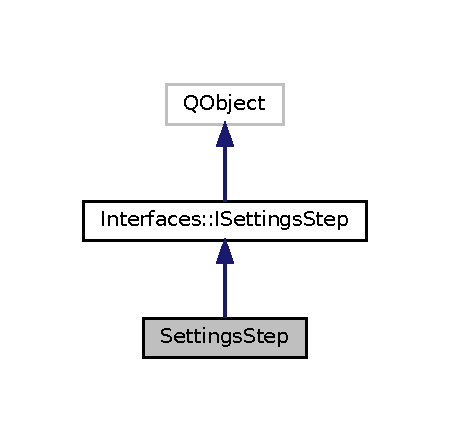
\includegraphics[width=216pt]{class_settings_step__inherit__graph}
\end{center}
\end{figure}


Collaboration diagram for Settings\+Step\+:\nopagebreak
\begin{figure}[H]
\begin{center}
\leavevmode
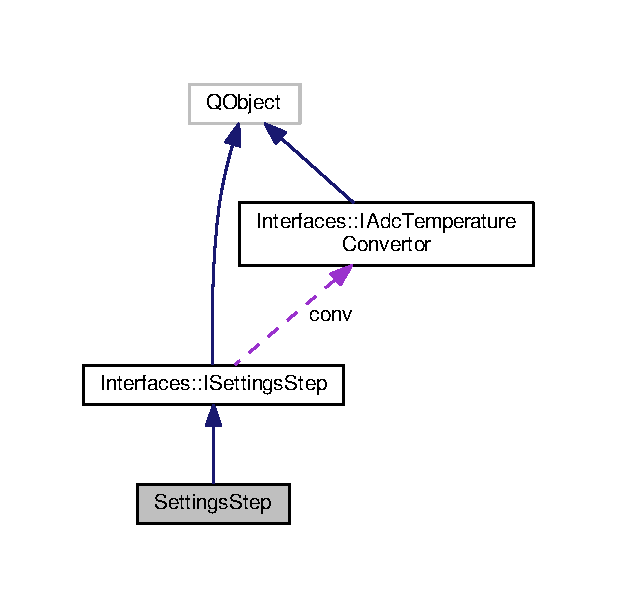
\includegraphics[width=314pt]{class_settings_step__coll__graph}
\end{center}
\end{figure}
\subsection*{Public Member Functions}
\begin{DoxyCompactItemize}
\item 
\mbox{\Hypertarget{class_settings_step_a5239f429f2c4abe89ddd16bedb77fce9}\label{class_settings_step_a5239f429f2c4abe89ddd16bedb77fce9}} 
{\bfseries Settings\+Step} (\hyperlink{class_interfaces_1_1_i_adc_temperature_convertor}{Interfaces\+::\+I\+Adc\+Temperature\+Convertor} $\ast$\hyperlink{class_interfaces_1_1_i_settings_step_aaa28fcd5fc0d1ed075ad2e274dd5ca01}{\+\_\+conv})
\item 
void \hyperlink{class_settings_step_ac6f79a139ab25cc50ed105f64fc9652f}{Calculate\+Primary\+Values} (uint previous\+\_\+adc, uint previous\+\_\+rpm)
\begin{DoxyCompactList}\small\item\em Calculates primary values (i.\+e. current A\+DC level and current R\+PM) basing on previus step values. If resulting A\+DC / R\+PM levels will be greater than A\+D\+C\+\_\+\+M\+A\+X\+\_\+\+V\+A\+L\+UE / M\+A\+X\+\_\+\+R\+PM respectively, then levels will be set to A\+D\+C\+\_\+\+M\+A\+X\+\_\+\+V\+A\+L\+UE / M\+A\+X\+\_\+\+R\+PM. \end{DoxyCompactList}\item 
Q\+String \hyperlink{class_settings_step_a21e452401e180d6e114561a8b05ab1ae}{Get\+Current\+R\+P\+M\+Percents\+String} ()
\begin{DoxyCompactList}\small\item\em Returns \char`\"{}\+Off\char`\"{} if \+\_\+\+Current\+R\+PM == 0, and string representation of \hyperlink{class_settings_step_a35bea9115637a0c848e8f827f2353c11}{Get\+Current\+R\+P\+M\+Percents()} otherwise. \end{DoxyCompactList}\item 
void \hyperlink{class_settings_step_a8124c87ae0b1d9fb3b623144d0e492db}{Set\+A\+D\+C\+Delta} (uint delta, bool skip\+Limits\+Check=false)
\begin{DoxyCompactList}\small\item\em Call it to set A\+DC delta value. If delta more than M\+A\+X\+\_\+\+A\+D\+C\+\_\+\+D\+E\+L\+TA (defined in descendant) set it to M\+A\+X\+\_\+\+A\+D\+C\+\_\+\+D\+E\+L\+TA, if it less then M\+I\+N\+\_\+\+A\+D\+C\+\_\+\+D\+E\+L\+TA -\/ set it to M\+I\+N\+\_\+\+A\+D\+C\+\_\+\+D\+E\+L\+TA. \end{DoxyCompactList}\item 
uint \hyperlink{class_settings_step_a443f5643d9b547632c261c5f3a4288f1}{Get\+Current\+A\+DC} ()
\begin{DoxyCompactList}\small\item\em Returns A\+DC level for this step. \end{DoxyCompactList}\item 
double \hyperlink{class_settings_step_a78ec872aa61713e3df36e93f56804afe}{Get\+Current\+Temperature} ()
\begin{DoxyCompactList}\small\item\em As \hyperlink{class_settings_step_a443f5643d9b547632c261c5f3a4288f1}{Get\+Current\+A\+D\+C()}, but returns temperature in Celsius. \end{DoxyCompactList}\item 
uint \hyperlink{class_settings_step_aee30aaa97692d6b546e9dd002900f52e}{Get\+A\+D\+C\+Delta} ()
\begin{DoxyCompactList}\small\item\em Returns current A\+DC delta. \end{DoxyCompactList}\item 
double \hyperlink{class_settings_step_a8162810e5ce2df99053ac5722acc0901}{Get\+Temp\+Delta} ()
\begin{DoxyCompactList}\small\item\em As \hyperlink{class_settings_step_aee30aaa97692d6b546e9dd002900f52e}{Get\+A\+D\+C\+Delta()}, but returns current A\+DC delta, converted to Celsius. \end{DoxyCompactList}\item 
void \hyperlink{class_settings_step_a25ddaf1d4d77727b8f87b5f8588f2de1}{Set\+R\+P\+M\+Delta} (uint delta, bool skip\+Limits\+Check=false)
\begin{DoxyCompactList}\small\item\em Like \hyperlink{class_settings_step_a8124c87ae0b1d9fb3b623144d0e492db}{Set\+A\+D\+C\+Delta()}, but for R\+PM delta. Making check for M\+A\+X\+\_\+\+R\+P\+M\+\_\+\+D\+E\+L\+TA, if delta is greater then it, delta will be M\+A\+X\+\_\+\+R\+P\+M\+\_\+\+D\+E\+L\+TA. \end{DoxyCompactList}\item 
uint \hyperlink{class_settings_step_aaba560b593af9bc96eeed3db01a469f4}{Get\+Current\+R\+PM} ()
\begin{DoxyCompactList}\small\item\em Get current R\+PM setting (see \hyperlink{_i_settings_generator_8hpp_source}{Interfaces/\+I\+Settings\+Generator.\+hpp} for details) \end{DoxyCompactList}\item 
double \hyperlink{class_settings_step_a35bea9115637a0c848e8f827f2353c11}{Get\+Current\+R\+P\+M\+Percents} ()
\begin{DoxyCompactList}\small\item\em As \hyperlink{class_settings_step_aaba560b593af9bc96eeed3db01a469f4}{Get\+Current\+R\+P\+M()}, but returns value in percents. \end{DoxyCompactList}\item 
uint \hyperlink{class_settings_step_a594ce71fb0626c79c3e4d4f988e484af}{Get\+R\+P\+M\+Delta} ()
\begin{DoxyCompactList}\small\item\em As \hyperlink{class_settings_step_aee30aaa97692d6b546e9dd002900f52e}{Get\+A\+D\+C\+Delta()}, but for R\+PM delta. \end{DoxyCompactList}\item 
double \hyperlink{class_settings_step_ada359fe4bfdaf271e621ec2943c0644c}{Get\+R\+P\+M\+Delta\+Percents} ()
\begin{DoxyCompactList}\small\item\em As \hyperlink{class_settings_step_a594ce71fb0626c79c3e4d4f988e484af}{Get\+R\+P\+M\+Delta()}, but in percents. \end{DoxyCompactList}\end{DoxyCompactItemize}
\subsection*{Additional Inherited Members}


\subsection{Detailed Description}
Class with one settings step (see Interfaces/\+I\+Settings\+Step for information) 

Definition at line 64 of file Settings\+Step.\+hpp.



\subsection{Member Function Documentation}
\mbox{\Hypertarget{class_settings_step_ac6f79a139ab25cc50ed105f64fc9652f}\label{class_settings_step_ac6f79a139ab25cc50ed105f64fc9652f}} 
\index{Settings\+Step@{Settings\+Step}!Calculate\+Primary\+Values@{Calculate\+Primary\+Values}}
\index{Calculate\+Primary\+Values@{Calculate\+Primary\+Values}!Settings\+Step@{Settings\+Step}}
\subsubsection{\texorpdfstring{Calculate\+Primary\+Values()}{CalculatePrimaryValues()}}
{\footnotesize\ttfamily void Settings\+Step\+::\+Calculate\+Primary\+Values (\begin{DoxyParamCaption}\item[{uint}]{previous\+\_\+adc,  }\item[{uint}]{previous\+\_\+rpm }\end{DoxyParamCaption})\hspace{0.3cm}{\ttfamily [virtual]}}



Calculates primary values (i.\+e. current A\+DC level and current R\+PM) basing on previus step values. If resulting A\+DC / R\+PM levels will be greater than A\+D\+C\+\_\+\+M\+A\+X\+\_\+\+V\+A\+L\+UE / M\+A\+X\+\_\+\+R\+PM respectively, then levels will be set to A\+D\+C\+\_\+\+M\+A\+X\+\_\+\+V\+A\+L\+UE / M\+A\+X\+\_\+\+R\+PM. 


\begin{DoxyParams}{Parameters}
{\em previous\+\_\+adc} & Previous step A\+DC value \\
\hline
{\em previous\+\_\+rpm} & Previous step R\+PM value \\
\hline
\end{DoxyParams}


Implements \hyperlink{class_interfaces_1_1_i_settings_step_a04e46c3ebe1f28e0ad0bce23fb863f66}{Interfaces\+::\+I\+Settings\+Step}.



Definition at line 43 of file Settings\+Step.\+cpp.

\mbox{\Hypertarget{class_settings_step_aee30aaa97692d6b546e9dd002900f52e}\label{class_settings_step_aee30aaa97692d6b546e9dd002900f52e}} 
\index{Settings\+Step@{Settings\+Step}!Get\+A\+D\+C\+Delta@{Get\+A\+D\+C\+Delta}}
\index{Get\+A\+D\+C\+Delta@{Get\+A\+D\+C\+Delta}!Settings\+Step@{Settings\+Step}}
\subsubsection{\texorpdfstring{Get\+A\+D\+C\+Delta()}{GetADCDelta()}}
{\footnotesize\ttfamily uint Settings\+Step\+::\+Get\+A\+D\+C\+Delta (\begin{DoxyParamCaption}{ }\end{DoxyParamCaption})\hspace{0.3cm}{\ttfamily [virtual]}}



Returns current A\+DC delta. 

\begin{DoxyReturn}{Returns}
A\+DC delta for this step 
\end{DoxyReturn}


Implements \hyperlink{class_interfaces_1_1_i_settings_step_ab77c6eaa45707ec4932a8f432b13ad78}{Interfaces\+::\+I\+Settings\+Step}.



Definition at line 87 of file Settings\+Step.\+cpp.

\mbox{\Hypertarget{class_settings_step_a443f5643d9b547632c261c5f3a4288f1}\label{class_settings_step_a443f5643d9b547632c261c5f3a4288f1}} 
\index{Settings\+Step@{Settings\+Step}!Get\+Current\+A\+DC@{Get\+Current\+A\+DC}}
\index{Get\+Current\+A\+DC@{Get\+Current\+A\+DC}!Settings\+Step@{Settings\+Step}}
\subsubsection{\texorpdfstring{Get\+Current\+A\+D\+C()}{GetCurrentADC()}}
{\footnotesize\ttfamily uint Settings\+Step\+::\+Get\+Current\+A\+DC (\begin{DoxyParamCaption}{ }\end{DoxyParamCaption})\hspace{0.3cm}{\ttfamily [virtual]}}



Returns A\+DC level for this step. 

\begin{DoxyReturn}{Returns}
A\+DC level for this step 
\end{DoxyReturn}


Implements \hyperlink{class_interfaces_1_1_i_settings_step_a54d5ce3350791e080bcb75d472376abf}{Interfaces\+::\+I\+Settings\+Step}.



Definition at line 116 of file Settings\+Step.\+cpp.

\mbox{\Hypertarget{class_settings_step_aaba560b593af9bc96eeed3db01a469f4}\label{class_settings_step_aaba560b593af9bc96eeed3db01a469f4}} 
\index{Settings\+Step@{Settings\+Step}!Get\+Current\+R\+PM@{Get\+Current\+R\+PM}}
\index{Get\+Current\+R\+PM@{Get\+Current\+R\+PM}!Settings\+Step@{Settings\+Step}}
\subsubsection{\texorpdfstring{Get\+Current\+R\+P\+M()}{GetCurrentRPM()}}
{\footnotesize\ttfamily uint Settings\+Step\+::\+Get\+Current\+R\+PM (\begin{DoxyParamCaption}{ }\end{DoxyParamCaption})\hspace{0.3cm}{\ttfamily [virtual]}}



Get current R\+PM setting (see \hyperlink{_i_settings_generator_8hpp_source}{Interfaces/\+I\+Settings\+Generator.\+hpp} for details) 

\begin{DoxyReturn}{Returns}
Current step R\+PM setting 
\end{DoxyReturn}


Implements \hyperlink{class_interfaces_1_1_i_settings_step_ac2b2370bf70fb09a9e1da4db922e8903}{Interfaces\+::\+I\+Settings\+Step}.



Definition at line 121 of file Settings\+Step.\+cpp.

\mbox{\Hypertarget{class_settings_step_a35bea9115637a0c848e8f827f2353c11}\label{class_settings_step_a35bea9115637a0c848e8f827f2353c11}} 
\index{Settings\+Step@{Settings\+Step}!Get\+Current\+R\+P\+M\+Percents@{Get\+Current\+R\+P\+M\+Percents}}
\index{Get\+Current\+R\+P\+M\+Percents@{Get\+Current\+R\+P\+M\+Percents}!Settings\+Step@{Settings\+Step}}
\subsubsection{\texorpdfstring{Get\+Current\+R\+P\+M\+Percents()}{GetCurrentRPMPercents()}}
{\footnotesize\ttfamily double Settings\+Step\+::\+Get\+Current\+R\+P\+M\+Percents (\begin{DoxyParamCaption}{ }\end{DoxyParamCaption})\hspace{0.3cm}{\ttfamily [virtual]}}



As \hyperlink{class_settings_step_aaba560b593af9bc96eeed3db01a469f4}{Get\+Current\+R\+P\+M()}, but returns value in percents. 

\begin{DoxyReturn}{Returns}
Current step R\+PM setting in percents 
\end{DoxyReturn}


Implements \hyperlink{class_interfaces_1_1_i_settings_step_abbbb49e91352212c6201a85f1a22253f}{Interfaces\+::\+I\+Settings\+Step}.



Definition at line 136 of file Settings\+Step.\+cpp.

\mbox{\Hypertarget{class_settings_step_a21e452401e180d6e114561a8b05ab1ae}\label{class_settings_step_a21e452401e180d6e114561a8b05ab1ae}} 
\index{Settings\+Step@{Settings\+Step}!Get\+Current\+R\+P\+M\+Percents\+String@{Get\+Current\+R\+P\+M\+Percents\+String}}
\index{Get\+Current\+R\+P\+M\+Percents\+String@{Get\+Current\+R\+P\+M\+Percents\+String}!Settings\+Step@{Settings\+Step}}
\subsubsection{\texorpdfstring{Get\+Current\+R\+P\+M\+Percents\+String()}{GetCurrentRPMPercentsString()}}
{\footnotesize\ttfamily Q\+String Settings\+Step\+::\+Get\+Current\+R\+P\+M\+Percents\+String (\begin{DoxyParamCaption}{ }\end{DoxyParamCaption})\hspace{0.3cm}{\ttfamily [virtual]}}



Returns \char`\"{}\+Off\char`\"{} if \+\_\+\+Current\+R\+PM == 0, and string representation of \hyperlink{class_settings_step_a35bea9115637a0c848e8f827f2353c11}{Get\+Current\+R\+P\+M\+Percents()} otherwise. 

\begin{DoxyReturn}{Returns}
\char`\"{}\+Off\char`\"{} or current R\+P\+Ms as string with percents 
\end{DoxyReturn}


Implements \hyperlink{class_interfaces_1_1_i_settings_step_a7575d43b7d178d700e161ec48e2c766f}{Interfaces\+::\+I\+Settings\+Step}.



Definition at line 59 of file Settings\+Step.\+cpp.

\mbox{\Hypertarget{class_settings_step_a78ec872aa61713e3df36e93f56804afe}\label{class_settings_step_a78ec872aa61713e3df36e93f56804afe}} 
\index{Settings\+Step@{Settings\+Step}!Get\+Current\+Temperature@{Get\+Current\+Temperature}}
\index{Get\+Current\+Temperature@{Get\+Current\+Temperature}!Settings\+Step@{Settings\+Step}}
\subsubsection{\texorpdfstring{Get\+Current\+Temperature()}{GetCurrentTemperature()}}
{\footnotesize\ttfamily double Settings\+Step\+::\+Get\+Current\+Temperature (\begin{DoxyParamCaption}{ }\end{DoxyParamCaption})\hspace{0.3cm}{\ttfamily [virtual]}}



As \hyperlink{class_settings_step_a443f5643d9b547632c261c5f3a4288f1}{Get\+Current\+A\+D\+C()}, but returns temperature in Celsius. 

\begin{DoxyReturn}{Returns}
Current step temperature in Celsius 
\end{DoxyReturn}


Implements \hyperlink{class_interfaces_1_1_i_settings_step_a62644690b7b63d27e72eca277a32bfdd}{Interfaces\+::\+I\+Settings\+Step}.



Definition at line 131 of file Settings\+Step.\+cpp.

\mbox{\Hypertarget{class_settings_step_a594ce71fb0626c79c3e4d4f988e484af}\label{class_settings_step_a594ce71fb0626c79c3e4d4f988e484af}} 
\index{Settings\+Step@{Settings\+Step}!Get\+R\+P\+M\+Delta@{Get\+R\+P\+M\+Delta}}
\index{Get\+R\+P\+M\+Delta@{Get\+R\+P\+M\+Delta}!Settings\+Step@{Settings\+Step}}
\subsubsection{\texorpdfstring{Get\+R\+P\+M\+Delta()}{GetRPMDelta()}}
{\footnotesize\ttfamily uint Settings\+Step\+::\+Get\+R\+P\+M\+Delta (\begin{DoxyParamCaption}{ }\end{DoxyParamCaption})\hspace{0.3cm}{\ttfamily [virtual]}}



As \hyperlink{class_settings_step_aee30aaa97692d6b546e9dd002900f52e}{Get\+A\+D\+C\+Delta()}, but for R\+PM delta. 

\begin{DoxyReturn}{Returns}
R\+PM delta for this step 
\end{DoxyReturn}


Implements \hyperlink{class_interfaces_1_1_i_settings_step_ace758dafae2a6bcbb0b1a3a64c802e3c}{Interfaces\+::\+I\+Settings\+Step}.



Definition at line 111 of file Settings\+Step.\+cpp.

\mbox{\Hypertarget{class_settings_step_ada359fe4bfdaf271e621ec2943c0644c}\label{class_settings_step_ada359fe4bfdaf271e621ec2943c0644c}} 
\index{Settings\+Step@{Settings\+Step}!Get\+R\+P\+M\+Delta\+Percents@{Get\+R\+P\+M\+Delta\+Percents}}
\index{Get\+R\+P\+M\+Delta\+Percents@{Get\+R\+P\+M\+Delta\+Percents}!Settings\+Step@{Settings\+Step}}
\subsubsection{\texorpdfstring{Get\+R\+P\+M\+Delta\+Percents()}{GetRPMDeltaPercents()}}
{\footnotesize\ttfamily double Settings\+Step\+::\+Get\+R\+P\+M\+Delta\+Percents (\begin{DoxyParamCaption}{ }\end{DoxyParamCaption})\hspace{0.3cm}{\ttfamily [virtual]}}



As \hyperlink{class_settings_step_a594ce71fb0626c79c3e4d4f988e484af}{Get\+R\+P\+M\+Delta()}, but in percents. 

\begin{DoxyReturn}{Returns}
R\+PM delta for this step in percents 
\end{DoxyReturn}


Implements \hyperlink{class_interfaces_1_1_i_settings_step_a9db8c7569c5dc35b8541dc6e4d202df1}{Interfaces\+::\+I\+Settings\+Step}.



Definition at line 126 of file Settings\+Step.\+cpp.

\mbox{\Hypertarget{class_settings_step_a8162810e5ce2df99053ac5722acc0901}\label{class_settings_step_a8162810e5ce2df99053ac5722acc0901}} 
\index{Settings\+Step@{Settings\+Step}!Get\+Temp\+Delta@{Get\+Temp\+Delta}}
\index{Get\+Temp\+Delta@{Get\+Temp\+Delta}!Settings\+Step@{Settings\+Step}}
\subsubsection{\texorpdfstring{Get\+Temp\+Delta()}{GetTempDelta()}}
{\footnotesize\ttfamily double Settings\+Step\+::\+Get\+Temp\+Delta (\begin{DoxyParamCaption}{ }\end{DoxyParamCaption})\hspace{0.3cm}{\ttfamily [virtual]}}



As \hyperlink{class_settings_step_aee30aaa97692d6b546e9dd002900f52e}{Get\+A\+D\+C\+Delta()}, but returns current A\+DC delta, converted to Celsius. 

\begin{DoxyReturn}{Returns}
Celsuis representation of A\+DC delta 
\end{DoxyReturn}


Implements \hyperlink{class_interfaces_1_1_i_settings_step_a7dd93517fbd9bc10a54b3b35a2f8bd78}{Interfaces\+::\+I\+Settings\+Step}.



Definition at line 92 of file Settings\+Step.\+cpp.

\mbox{\Hypertarget{class_settings_step_a8124c87ae0b1d9fb3b623144d0e492db}\label{class_settings_step_a8124c87ae0b1d9fb3b623144d0e492db}} 
\index{Settings\+Step@{Settings\+Step}!Set\+A\+D\+C\+Delta@{Set\+A\+D\+C\+Delta}}
\index{Set\+A\+D\+C\+Delta@{Set\+A\+D\+C\+Delta}!Settings\+Step@{Settings\+Step}}
\subsubsection{\texorpdfstring{Set\+A\+D\+C\+Delta()}{SetADCDelta()}}
{\footnotesize\ttfamily void Settings\+Step\+::\+Set\+A\+D\+C\+Delta (\begin{DoxyParamCaption}\item[{uint}]{delta,  }\item[{bool}]{skip\+Limits\+Check = {\ttfamily false} }\end{DoxyParamCaption})\hspace{0.3cm}{\ttfamily [virtual]}}



Call it to set A\+DC delta value. If delta more than M\+A\+X\+\_\+\+A\+D\+C\+\_\+\+D\+E\+L\+TA (defined in descendant) set it to M\+A\+X\+\_\+\+A\+D\+C\+\_\+\+D\+E\+L\+TA, if it less then M\+I\+N\+\_\+\+A\+D\+C\+\_\+\+D\+E\+L\+TA -\/ set it to M\+I\+N\+\_\+\+A\+D\+C\+\_\+\+D\+E\+L\+TA. 


\begin{DoxyParams}{Parameters}
{\em delta} & This value added to A\+DC value when we are going to next step (see Firmware/main.\+h E\+E\+P\+R\+OM S\+T\+R\+U\+C\+T\+U\+RE section for description) \\
\hline
{\em skip\+Limits\+Check} & If set to true, then checks for M\+I\+N\+\_\+\+A\+D\+C\+\_\+\+D\+E\+L\+TA and M\+A\+X\+\_\+\+A\+D\+C\+\_\+\+D\+E\+L\+TA will be skipped. Us it only for setting base level, because values outside \mbox{[}M\+I\+N\+\_\+\+A\+D\+C\+\_\+\+D\+E\+L\+T\+A-\/\+M\+A\+X\+\_\+\+A\+D\+C\+\_\+\+D\+E\+L\+TA\mbox{]} can\textquotesingle{}t be programmed into M\+CU. \\
\hline
\end{DoxyParams}


Implements \hyperlink{class_interfaces_1_1_i_settings_step_a83f00b8b66f6566721065e34e41508c6}{Interfaces\+::\+I\+Settings\+Step}.



Definition at line 69 of file Settings\+Step.\+cpp.

\mbox{\Hypertarget{class_settings_step_a25ddaf1d4d77727b8f87b5f8588f2de1}\label{class_settings_step_a25ddaf1d4d77727b8f87b5f8588f2de1}} 
\index{Settings\+Step@{Settings\+Step}!Set\+R\+P\+M\+Delta@{Set\+R\+P\+M\+Delta}}
\index{Set\+R\+P\+M\+Delta@{Set\+R\+P\+M\+Delta}!Settings\+Step@{Settings\+Step}}
\subsubsection{\texorpdfstring{Set\+R\+P\+M\+Delta()}{SetRPMDelta()}}
{\footnotesize\ttfamily void Settings\+Step\+::\+Set\+R\+P\+M\+Delta (\begin{DoxyParamCaption}\item[{uint}]{delta,  }\item[{bool}]{skip\+Limits\+Check = {\ttfamily false} }\end{DoxyParamCaption})\hspace{0.3cm}{\ttfamily [virtual]}}



Like \hyperlink{class_settings_step_a8124c87ae0b1d9fb3b623144d0e492db}{Set\+A\+D\+C\+Delta()}, but for R\+PM delta. Making check for M\+A\+X\+\_\+\+R\+P\+M\+\_\+\+D\+E\+L\+TA, if delta is greater then it, delta will be M\+A\+X\+\_\+\+R\+P\+M\+\_\+\+D\+E\+L\+TA. 


\begin{DoxyParams}{Parameters}
{\em delta} & This value added to R\+PM raw value when we are going to next step (see Firmware/main.\+h E\+E\+P\+R\+OM S\+T\+R\+U\+C\+T\+U\+RE section for description) \\
\hline
\end{DoxyParams}


Implements \hyperlink{class_interfaces_1_1_i_settings_step_a62997701dc6ad91ec0a9d699ef99463e}{Interfaces\+::\+I\+Settings\+Step}.



Definition at line 97 of file Settings\+Step.\+cpp.



The documentation for this class was generated from the following files\+:\begin{DoxyCompactItemize}
\item 
Implementations/Settings\+Step.\+hpp\item 
Implementations/Settings\+Step.\+cpp\end{DoxyCompactItemize}

%--- End generated contents ---

% Index
\backmatter
\newpage
\phantomsection
\clearemptydoublepage
\addcontentsline{toc}{chapter}{Index}
\printindex

\end{document}
